
\documentclass{article}
\usepackage{enumitem}
\usepackage{iclr2026_conference,times}

% Optional math commands from https://github.com/goodfeli/dlbook_notation.
%%%%% NEW MATH DEFINITIONS %%%%%

\usepackage{amsmath,amsfonts,bm}

% Mark sections of captions for referring to divisions of figures
\newcommand{\figleft}{{\em (Left)}}
\newcommand{\figcenter}{{\em (Center)}}
\newcommand{\figright}{{\em (Right)}}
\newcommand{\figtop}{{\em (Top)}}
\newcommand{\figbottom}{{\em (Bottom)}}
\newcommand{\captiona}{{\em (a)}}
\newcommand{\captionb}{{\em (b)}}
\newcommand{\captionc}{{\em (c)}}
\newcommand{\captiond}{{\em (d)}}

% Highlight a newly defined term
\newcommand{\newterm}[1]{{\bf #1}}


% Figure reference, lower-case.
\def\figref#1{figure~\ref{#1}}
% Figure reference, capital. For start of sentence
\def\Figref#1{Figure~\ref{#1}}
\def\twofigref#1#2{figures \ref{#1} and \ref{#2}}
\def\quadfigref#1#2#3#4{figures \ref{#1}, \ref{#2}, \ref{#3} and \ref{#4}}
% Section reference, lower-case.
\def\secref#1{section~\ref{#1}}
% Section reference, capital.
\def\Secref#1{Section~\ref{#1}}
% Reference to two sections.
\def\twosecrefs#1#2{sections \ref{#1} and \ref{#2}}
% Reference to three sections.
\def\secrefs#1#2#3{sections \ref{#1}, \ref{#2} and \ref{#3}}
% Reference to an equation, lower-case.
\def\eqref#1{equation~\ref{#1}}
% Reference to an equation, upper case
\def\Eqref#1{Equation~\ref{#1}}
% A raw reference to an equation---avoid using if possible
\def\plaineqref#1{\ref{#1}}
% Reference to a chapter, lower-case.
\def\chapref#1{chapter~\ref{#1}}
% Reference to an equation, upper case.
\def\Chapref#1{Chapter~\ref{#1}}
% Reference to a range of chapters
\def\rangechapref#1#2{chapters\ref{#1}--\ref{#2}}
% Reference to an algorithm, lower-case.
\def\algref#1{algorithm~\ref{#1}}
% Reference to an algorithm, upper case.
\def\Algref#1{Algorithm~\ref{#1}}
\def\twoalgref#1#2{algorithms \ref{#1} and \ref{#2}}
\def\Twoalgref#1#2{Algorithms \ref{#1} and \ref{#2}}
% Reference to a part, lower case
\def\partref#1{part~\ref{#1}}
% Reference to a part, upper case
\def\Partref#1{Part~\ref{#1}}
\def\twopartref#1#2{parts \ref{#1} and \ref{#2}}

\def\ceil#1{\lceil #1 \rceil}
\def\floor#1{\lfloor #1 \rfloor}
\def\1{\bm{1}}
\newcommand{\train}{\mathcal{D}}
\newcommand{\valid}{\mathcal{D_{\mathrm{valid}}}}
\newcommand{\test}{\mathcal{D_{\mathrm{test}}}}

\def\eps{{\epsilon}}


% Random variables
\def\reta{{\textnormal{$\eta$}}}
\def\ra{{\textnormal{a}}}
\def\rb{{\textnormal{b}}}
\def\rc{{\textnormal{c}}}
\def\rd{{\textnormal{d}}}
\def\re{{\textnormal{e}}}
\def\rf{{\textnormal{f}}}
\def\rg{{\textnormal{g}}}
\def\rh{{\textnormal{h}}}
\def\ri{{\textnormal{i}}}
\def\rj{{\textnormal{j}}}
\def\rk{{\textnormal{k}}}
\def\rl{{\textnormal{l}}}
% rm is already a command, just don't name any random variables m
\def\rn{{\textnormal{n}}}
\def\ro{{\textnormal{o}}}
\def\rp{{\textnormal{p}}}
\def\rq{{\textnormal{q}}}
\def\rr{{\textnormal{r}}}
\def\rs{{\textnormal{s}}}
\def\rt{{\textnormal{t}}}
\def\ru{{\textnormal{u}}}
\def\rv{{\textnormal{v}}}
\def\rw{{\textnormal{w}}}
\def\rx{{\textnormal{x}}}
\def\ry{{\textnormal{y}}}
\def\rz{{\textnormal{z}}}

% Random vectors
\def\rvepsilon{{\mathbf{\epsilon}}}
\def\rvtheta{{\mathbf{\theta}}}
\def\rva{{\mathbf{a}}}
\def\rvb{{\mathbf{b}}}
\def\rvc{{\mathbf{c}}}
\def\rvd{{\mathbf{d}}}
\def\rve{{\mathbf{e}}}
\def\rvf{{\mathbf{f}}}
\def\rvg{{\mathbf{g}}}
\def\rvh{{\mathbf{h}}}
\def\rvu{{\mathbf{i}}}
\def\rvj{{\mathbf{j}}}
\def\rvk{{\mathbf{k}}}
\def\rvl{{\mathbf{l}}}
\def\rvm{{\mathbf{m}}}
\def\rvn{{\mathbf{n}}}
\def\rvo{{\mathbf{o}}}
\def\rvp{{\mathbf{p}}}
\def\rvq{{\mathbf{q}}}
\def\rvr{{\mathbf{r}}}
\def\rvs{{\mathbf{s}}}
\def\rvt{{\mathbf{t}}}
\def\rvu{{\mathbf{u}}}
\def\rvv{{\mathbf{v}}}
\def\rvw{{\mathbf{w}}}
\def\rvx{{\mathbf{x}}}
\def\rvy{{\mathbf{y}}}
\def\rvz{{\mathbf{z}}}

% Elements of random vectors
\def\erva{{\textnormal{a}}}
\def\ervb{{\textnormal{b}}}
\def\ervc{{\textnormal{c}}}
\def\ervd{{\textnormal{d}}}
\def\erve{{\textnormal{e}}}
\def\ervf{{\textnormal{f}}}
\def\ervg{{\textnormal{g}}}
\def\ervh{{\textnormal{h}}}
\def\ervi{{\textnormal{i}}}
\def\ervj{{\textnormal{j}}}
\def\ervk{{\textnormal{k}}}
\def\ervl{{\textnormal{l}}}
\def\ervm{{\textnormal{m}}}
\def\ervn{{\textnormal{n}}}
\def\ervo{{\textnormal{o}}}
\def\ervp{{\textnormal{p}}}
\def\ervq{{\textnormal{q}}}
\def\ervr{{\textnormal{r}}}
\def\ervs{{\textnormal{s}}}
\def\ervt{{\textnormal{t}}}
\def\ervu{{\textnormal{u}}}
\def\ervv{{\textnormal{v}}}
\def\ervw{{\textnormal{w}}}
\def\ervx{{\textnormal{x}}}
\def\ervy{{\textnormal{y}}}
\def\ervz{{\textnormal{z}}}

% Random matrices
\def\rmA{{\mathbf{A}}}
\def\rmB{{\mathbf{B}}}
\def\rmC{{\mathbf{C}}}
\def\rmD{{\mathbf{D}}}
\def\rmE{{\mathbf{E}}}
\def\rmF{{\mathbf{F}}}
\def\rmG{{\mathbf{G}}}
\def\rmH{{\mathbf{H}}}
\def\rmI{{\mathbf{I}}}
\def\rmJ{{\mathbf{J}}}
\def\rmK{{\mathbf{K}}}
\def\rmL{{\mathbf{L}}}
\def\rmM{{\mathbf{M}}}
\def\rmN{{\mathbf{N}}}
\def\rmO{{\mathbf{O}}}
\def\rmP{{\mathbf{P}}}
\def\rmQ{{\mathbf{Q}}}
\def\rmR{{\mathbf{R}}}
\def\rmS{{\mathbf{S}}}
\def\rmT{{\mathbf{T}}}
\def\rmU{{\mathbf{U}}}
\def\rmV{{\mathbf{V}}}
\def\rmW{{\mathbf{W}}}
\def\rmX{{\mathbf{X}}}
\def\rmY{{\mathbf{Y}}}
\def\rmZ{{\mathbf{Z}}}

% Elements of random matrices
\def\ermA{{\textnormal{A}}}
\def\ermB{{\textnormal{B}}}
\def\ermC{{\textnormal{C}}}
\def\ermD{{\textnormal{D}}}
\def\ermE{{\textnormal{E}}}
\def\ermF{{\textnormal{F}}}
\def\ermG{{\textnormal{G}}}
\def\ermH{{\textnormal{H}}}
\def\ermI{{\textnormal{I}}}
\def\ermJ{{\textnormal{J}}}
\def\ermK{{\textnormal{K}}}
\def\ermL{{\textnormal{L}}}
\def\ermM{{\textnormal{M}}}
\def\ermN{{\textnormal{N}}}
\def\ermO{{\textnormal{O}}}
\def\ermP{{\textnormal{P}}}
\def\ermQ{{\textnormal{Q}}}
\def\ermR{{\textnormal{R}}}
\def\ermS{{\textnormal{S}}}
\def\ermT{{\textnormal{T}}}
\def\ermU{{\textnormal{U}}}
\def\ermV{{\textnormal{V}}}
\def\ermW{{\textnormal{W}}}
\def\ermX{{\textnormal{X}}}
\def\ermY{{\textnormal{Y}}}
\def\ermZ{{\textnormal{Z}}}

% Vectors
\def\vzero{{\bm{0}}}
\def\vone{{\bm{1}}}
\def\vmu{{\bm{\mu}}}
\def\vtheta{{\bm{\theta}}}
\def\va{{\bm{a}}}
\def\vb{{\bm{b}}}
\def\vc{{\bm{c}}}
\def\vd{{\bm{d}}}
\def\ve{{\bm{e}}}
\def\vf{{\bm{f}}}
\def\vg{{\bm{g}}}
\def\vh{{\bm{h}}}
\def\vi{{\bm{i}}}
\def\vj{{\bm{j}}}
\def\vk{{\bm{k}}}
\def\vl{{\bm{l}}}
\def\vm{{\bm{m}}}
\def\vn{{\bm{n}}}
\def\vo{{\bm{o}}}
\def\vp{{\bm{p}}}
\def\vq{{\bm{q}}}
\def\vr{{\bm{r}}}
\def\vs{{\bm{s}}}
\def\vt{{\bm{t}}}
\def\vu{{\bm{u}}}
\def\vv{{\bm{v}}}
\def\vw{{\bm{w}}}
\def\vx{{\bm{x}}}
\def\vy{{\bm{y}}}
\def\vz{{\bm{z}}}

% Elements of vectors
\def\evalpha{{\alpha}}
\def\evbeta{{\beta}}
\def\evepsilon{{\epsilon}}
\def\evlambda{{\lambda}}
\def\evomega{{\omega}}
\def\evmu{{\mu}}
\def\evpsi{{\psi}}
\def\evsigma{{\sigma}}
\def\evtheta{{\theta}}
\def\eva{{a}}
\def\evb{{b}}
\def\evc{{c}}
\def\evd{{d}}
\def\eve{{e}}
\def\evf{{f}}
\def\evg{{g}}
\def\evh{{h}}
\def\evi{{i}}
\def\evj{{j}}
\def\evk{{k}}
\def\evl{{l}}
\def\evm{{m}}
\def\evn{{n}}
\def\evo{{o}}
\def\evp{{p}}
\def\evq{{q}}
\def\evr{{r}}
\def\evs{{s}}
\def\evt{{t}}
\def\evu{{u}}
\def\evv{{v}}
\def\evw{{w}}
\def\evx{{x}}
\def\evy{{y}}
\def\evz{{z}}

% Matrix
\def\mA{{\bm{A}}}
\def\mB{{\bm{B}}}
\def\mC{{\bm{C}}}
\def\mD{{\bm{D}}}
\def\mE{{\bm{E}}}
\def\mF{{\bm{F}}}
\def\mG{{\bm{G}}}
\def\mH{{\bm{H}}}
\def\mI{{\bm{I}}}
\def\mJ{{\bm{J}}}
\def\mK{{\bm{K}}}
\def\mL{{\bm{L}}}
\def\mM{{\bm{M}}}
\def\mN{{\bm{N}}}
\def\mO{{\bm{O}}}
\def\mP{{\bm{P}}}
\def\mQ{{\bm{Q}}}
\def\mR{{\bm{R}}}
\def\mS{{\bm{S}}}
\def\mT{{\bm{T}}}
\def\mU{{\bm{U}}}
\def\mV{{\bm{V}}}
\def\mW{{\bm{W}}}
\def\mX{{\bm{X}}}
\def\mY{{\bm{Y}}}
\def\mZ{{\bm{Z}}}
\def\mBeta{{\bm{\beta}}}
\def\mPhi{{\bm{\Phi}}}
\def\mLambda{{\bm{\Lambda}}}
\def\mSigma{{\bm{\Sigma}}}

% Tensor
\DeclareMathAlphabet{\mathsfit}{\encodingdefault}{\sfdefault}{m}{sl}
\SetMathAlphabet{\mathsfit}{bold}{\encodingdefault}{\sfdefault}{bx}{n}
\newcommand{\tens}[1]{\bm{\mathsfit{#1}}}
\def\tA{{\tens{A}}}
\def\tB{{\tens{B}}}
\def\tC{{\tens{C}}}
\def\tD{{\tens{D}}}
\def\tE{{\tens{E}}}
\def\tF{{\tens{F}}}
\def\tG{{\tens{G}}}
\def\tH{{\tens{H}}}
\def\tI{{\tens{I}}}
\def\tJ{{\tens{J}}}
\def\tK{{\tens{K}}}
\def\tL{{\tens{L}}}
\def\tM{{\tens{M}}}
\def\tN{{\tens{N}}}
\def\tO{{\tens{O}}}
\def\tP{{\tens{P}}}
\def\tQ{{\tens{Q}}}
\def\tR{{\tens{R}}}
\def\tS{{\tens{S}}}
\def\tT{{\tens{T}}}
\def\tU{{\tens{U}}}
\def\tV{{\tens{V}}}
\def\tW{{\tens{W}}}
\def\tX{{\tens{X}}}
\def\tY{{\tens{Y}}}
\def\tZ{{\tens{Z}}}


% Graph
\def\gA{{\mathcal{A}}}
\def\gB{{\mathcal{B}}}
\def\gC{{\mathcal{C}}}
\def\gD{{\mathcal{D}}}
\def\gE{{\mathcal{E}}}
\def\gF{{\mathcal{F}}}
\def\gG{{\mathcal{G}}}
\def\gH{{\mathcal{H}}}
\def\gI{{\mathcal{I}}}
\def\gJ{{\mathcal{J}}}
\def\gK{{\mathcal{K}}}
\def\gL{{\mathcal{L}}}
\def\gM{{\mathcal{M}}}
\def\gN{{\mathcal{N}}}
\def\gO{{\mathcal{O}}}
\def\gP{{\mathcal{P}}}
\def\gQ{{\mathcal{Q}}}
\def\gR{{\mathcal{R}}}
\def\gS{{\mathcal{S}}}
\def\gT{{\mathcal{T}}}
\def\gU{{\mathcal{U}}}
\def\gV{{\mathcal{V}}}
\def\gW{{\mathcal{W}}}
\def\gX{{\mathcal{X}}}
\def\gY{{\mathcal{Y}}}
\def\gZ{{\mathcal{Z}}}

% Sets
\def\sA{{\mathbb{A}}}
\def\sB{{\mathbb{B}}}
\def\sC{{\mathbb{C}}}
\def\sD{{\mathbb{D}}}
% Don't use a set called E, because this would be the same as our symbol
% for expectation.
\def\sF{{\mathbb{F}}}
\def\sG{{\mathbb{G}}}
\def\sH{{\mathbb{H}}}
\def\sI{{\mathbb{I}}}
\def\sJ{{\mathbb{J}}}
\def\sK{{\mathbb{K}}}
\def\sL{{\mathbb{L}}}
\def\sM{{\mathbb{M}}}
\def\sN{{\mathbb{N}}}
\def\sO{{\mathbb{O}}}
\def\sP{{\mathbb{P}}}
\def\sQ{{\mathbb{Q}}}
\def\sR{{\mathbb{R}}}
\def\sS{{\mathbb{S}}}
\def\sT{{\mathbb{T}}}
\def\sU{{\mathbb{U}}}
\def\sV{{\mathbb{V}}}
\def\sW{{\mathbb{W}}}
\def\sX{{\mathbb{X}}}
\def\sY{{\mathbb{Y}}}
\def\sZ{{\mathbb{Z}}}

% Entries of a matrix
\def\emLambda{{\Lambda}}
\def\emA{{A}}
\def\emB{{B}}
\def\emC{{C}}
\def\emD{{D}}
\def\emE{{E}}
\def\emF{{F}}
\def\emG{{G}}
\def\emH{{H}}
\def\emI{{I}}
\def\emJ{{J}}
\def\emK{{K}}
\def\emL{{L}}
\def\emM{{M}}
\def\emN{{N}}
\def\emO{{O}}
\def\emP{{P}}
\def\emQ{{Q}}
\def\emR{{R}}
\def\emS{{S}}
\def\emT{{T}}
\def\emU{{U}}
\def\emV{{V}}
\def\emW{{W}}
\def\emX{{X}}
\def\emY{{Y}}
\def\emZ{{Z}}
\def\emSigma{{\Sigma}}

% entries of a tensor
% Same font as tensor, without \bm wrapper
\newcommand{\etens}[1]{\mathsfit{#1}}
\def\etLambda{{\etens{\Lambda}}}
\def\etA{{\etens{A}}}
\def\etB{{\etens{B}}}
\def\etC{{\etens{C}}}
\def\etD{{\etens{D}}}
\def\etE{{\etens{E}}}
\def\etF{{\etens{F}}}
\def\etG{{\etens{G}}}
\def\etH{{\etens{H}}}
\def\etI{{\etens{I}}}
\def\etJ{{\etens{J}}}
\def\etK{{\etens{K}}}
\def\etL{{\etens{L}}}
\def\etM{{\etens{M}}}
\def\etN{{\etens{N}}}
\def\etO{{\etens{O}}}
\def\etP{{\etens{P}}}
\def\etQ{{\etens{Q}}}
\def\etR{{\etens{R}}}
\def\etS{{\etens{S}}}
\def\etT{{\etens{T}}}
\def\etU{{\etens{U}}}
\def\etV{{\etens{V}}}
\def\etW{{\etens{W}}}
\def\etX{{\etens{X}}}
\def\etY{{\etens{Y}}}
\def\etZ{{\etens{Z}}}

% The true underlying data generating distribution
\newcommand{\pdata}{p_{\rm{data}}}
% The empirical distribution defined by the training set
\newcommand{\ptrain}{\hat{p}_{\rm{data}}}
\newcommand{\Ptrain}{\hat{P}_{\rm{data}}}
% The model distribution
\newcommand{\pmodel}{p_{\rm{model}}}
\newcommand{\Pmodel}{P_{\rm{model}}}
\newcommand{\ptildemodel}{\tilde{p}_{\rm{model}}}
% Stochastic autoencoder distributions
\newcommand{\pencode}{p_{\rm{encoder}}}
\newcommand{\pdecode}{p_{\rm{decoder}}}
\newcommand{\precons}{p_{\rm{reconstruct}}}

\newcommand{\laplace}{\mathrm{Laplace}} % Laplace distribution

\newcommand{\E}{\mathbb{E}}
\newcommand{\Ls}{\mathcal{L}}
\newcommand{\R}{\mathbb{R}}
\newcommand{\emp}{\tilde{p}}
\newcommand{\lr}{\alpha}
\newcommand{\reg}{\lambda}
\newcommand{\rect}{\mathrm{rectifier}}
\newcommand{\softmax}{\mathrm{softmax}}
\newcommand{\sigmoid}{\sigma}
\newcommand{\softplus}{\zeta}
\newcommand{\KL}{D_{\mathrm{KL}}}
\newcommand{\Var}{\mathrm{Var}}
\newcommand{\standarderror}{\mathrm{SE}}
\newcommand{\Cov}{\mathrm{Cov}}
% Wolfram Mathworld says $L^2$ is for function spaces and $\ell^2$ is for vectors
% But then they seem to use $L^2$ for vectors throughout the site, and so does
% wikipedia.
\newcommand{\normlzero}{L^0}
\newcommand{\normlone}{L^1}
\newcommand{\normltwo}{L^2}
\newcommand{\normlp}{L^p}
\newcommand{\normmax}{L^\infty}

\newcommand{\parents}{Pa} % See usage in notation.tex. Chosen to match Daphne's book.

\DeclareMathOperator*{\argmax}{arg\,max}
\DeclareMathOperator*{\argmin}{arg\,min}

\DeclareMathOperator{\sign}{sign}
\DeclareMathOperator{\Tr}{Tr}
\let\ab\allowbreak

\usepackage{makecell} %
\usepackage{booktabs}
\usepackage[pagebackref=true,colorlinks,citecolor=brown]{hyperref}
% \usepackage{hyperref}
\usepackage{url}
\usepackage{graphicx}
\usepackage{amsfonts}
\usepackage{tabularx,booktabs,multirow}
% \usepackage{algorithm}
\usepackage{float}
\usepackage{overpic}
\usepackage{xcolor}
\usepackage{wrapfig}
\usepackage{nicefrac}
\usepackage{microtype}
\usepackage{xcolor}
\usepackage{enumitem}
\usepackage{amsmath,amssymb}
\usepackage{algorithm}
\usepackage[noend]{algpseudocode}
\usepackage{float}  
\usepackage{caption}
\captionsetup{font=small}
\usepackage{titlesec}
\usepackage{listings}
\usepackage[T1]{fontenc}
\usepackage{hyperref}
\usepackage{url}
\algrenewcommand{\algorithmiccomment}[1]{\hfill\(\triangleright\)~#1}

\renewcommand{\paragraph}[1]{\noindent\textbf{#1}.}
% Resolve figures from local ICLR project
\setlength{\abovedisplayskip}{2pt}
\setlength{\abovedisplayshortskip}{2pt}
\setlength{\belowdisplayskip}{2pt}
\setlength{\belowdisplayshortskip}{2pt}
\setlength{\textfloatsep}{1.5ex}
\titlespacing\section{0pt}{3pt plus 1pt minus 1pt}{2pt plus 1pt minus 1pt}
\titlespacing\subsection{0pt}{2pt plus 1pt minus 1pt}{1pt plus 1pt minus 1pt}
\setlength{\parskip}{0.45em}

\graphicspath{{Figures/}}


% \title{Compositional Language Architecture for  Reasoning}
\title{\NAME : Orchestrating Small Language Models for Reasoning}

% Authors and affiliations for arXiv version
% \author{
% Chenyu Wang\textsuperscript{1}\thanks{Equal contribution. Chenyu Wang designed the methodology and conducted all experiments. Zishen Wan initiated and coordinated the project, secured collaborations, and provided guidance.}\quad
% Zishen Wan\textsuperscript{2}\footnotemark[1]\quad
% Hao Kang\textsuperscript{2}\quad
% Emma Chen\textsuperscript{1}\quad
% Zhiqiang Xie\textsuperscript{3}\quad
% Tushar Krishna\textsuperscript{2}\quad
% Vijay Janapa Reddi\textsuperscript{1}\quad
% Yilun Du\textsuperscript{1}\thanks{Correspondence to: Yilun Du <ydu@seas.harvard.edu>.}\\
% \textsuperscript{1}Harvard University\quad
% \textsuperscript{2}Georgia Institute of Technology\quad
% \textsuperscript{3}Stanford University}
\author{%
\textbf{Chenyu Wang}$^{1}$\thanks{Equal contribution. Chenyu Wang designed the methodology and conducted all experiments. Zishen Wan initiated and coordinated the project, secured collaborations, and provided guidance.} \quad
\textbf{Zishen Wan}$^{2}$\footnotemark[1] \quad
\textbf{Hao Kang}$^{2}$ \quad
\textbf{Emma Chen}$^{1}$ \\
\textbf{Zhiqiang Xie}$^{3}$ \quad
\textbf{Tushar Krishna}$^{2}$ \quad
\textbf{Vijay Janapa Reddi}$^{1}$ \quad
\textbf{Yilun Du}$^{1}$\thanks{Correspondence to: Yilun Du <ydu@seas.harvard.edu>.} \\
\small $^{1}$Harvard University \quad $^{2}$Georgia Institute of Technology \quad $^{3}$Stanford University
}



\iclrfinalcopy % 摄影版就打开;匿名评审请注释掉



% The \author macro works with any number of authors. There are two commands
% used to separate the names and addresses of multiple authors: \And and \AND.
%
% Using \And between authors leaves it to \LaTeX{} to determine where to break
% the lines. Using \AND forces a linebreak at that point. So, if \LaTeX{}
% puts 3 of 4 authors names on the first line, and the last on the second
% line, try using \AND instead of \And before the third author name.

\newcommand{\fix}{\marginpar{FIX}}
\newcommand{\new}{\marginpar{NEW}}
\newcommand{\cw}[1]{\textcolor{magenta}{#1}}
\newcommand{\zishen}[1]{\textcolor{blue}{[ZW: #1}]}
\newcommand{\NAME}{\textsc{SLM-MUX}} 
\iclrfinalcopy % Uncomment for camera-ready version, but NOT for submission.



\begin{document}


\maketitle

% Use plain page style to suppress ICLR headers on arXiv
\thispagestyle{plain}
\pagestyle{plain}

\begin{abstract}
 With the rapid development of language models, the number of small language models (SLMs) has grown significantly. Although they do not achieve state-of-the-art accuracy, they are more efficient and often excel at specific tasks. This raises a natural question: can multiple SLMs be orchestrated into a system where each contributes effectively, achieving higher accuracy than any individual model? Existing orchestration methods have primarily targeted frontier models (e.g., GPT-4) and perform suboptimally when applied to SLMs. To address this gap, we propose a three-stage approach for orchestrating SLMs. First, we introduce \NAME{}, a multi-model architecture that effectively coordinates multiple SLMs. Building on this, we develop two optimization strategies: (i) a model selection search that identifies the most complementary SLMs from a given pool, and (ii) test-time scaling tailored to \NAME{}. Our approach delivers strong results: Compared to existing orchestration methods, our approach achieves up to 13.4\% improvement on MATH, 8.8\% on GPQA, and 7.0\% on GSM8K. With just two SLMs, \NAME{}  outperforms Qwen 2.5 72B on GPQA and GSM8K, and matches its performance on MATH. We further provide theoretical analyses to substantiate the advantages of our method. In summary, we demonstrate that SLMs can be effectively orchestrated into more accurate and efficient systems through the proposed approach. Project page and code: \url{https://slm-mux.github.io}.
\end{abstract}


% compared to best-performing SLMs in the system, our approach achieves up to 6.4\% improvement on MATH, 4.8\% on GPQA, and 5.7\% on GSM8K, using only two off-the-shelf SLMs. Compared to existing orchestration methods, our approach achieves up to 11.6\% improvement on MATH, 5.6\% on GPQA, and 6.8\% on GSM8K. We further provide theoretical analyses to substantiate the advantages of our method. In summary, we demonstrate that SLMs can be effectively orchestrated into more accurate and efficient systems through the proposed approach.

% ================= Our paper content begins here =================
\section{Introduction}
% \begin{figure}[htbp]
% \centering
% 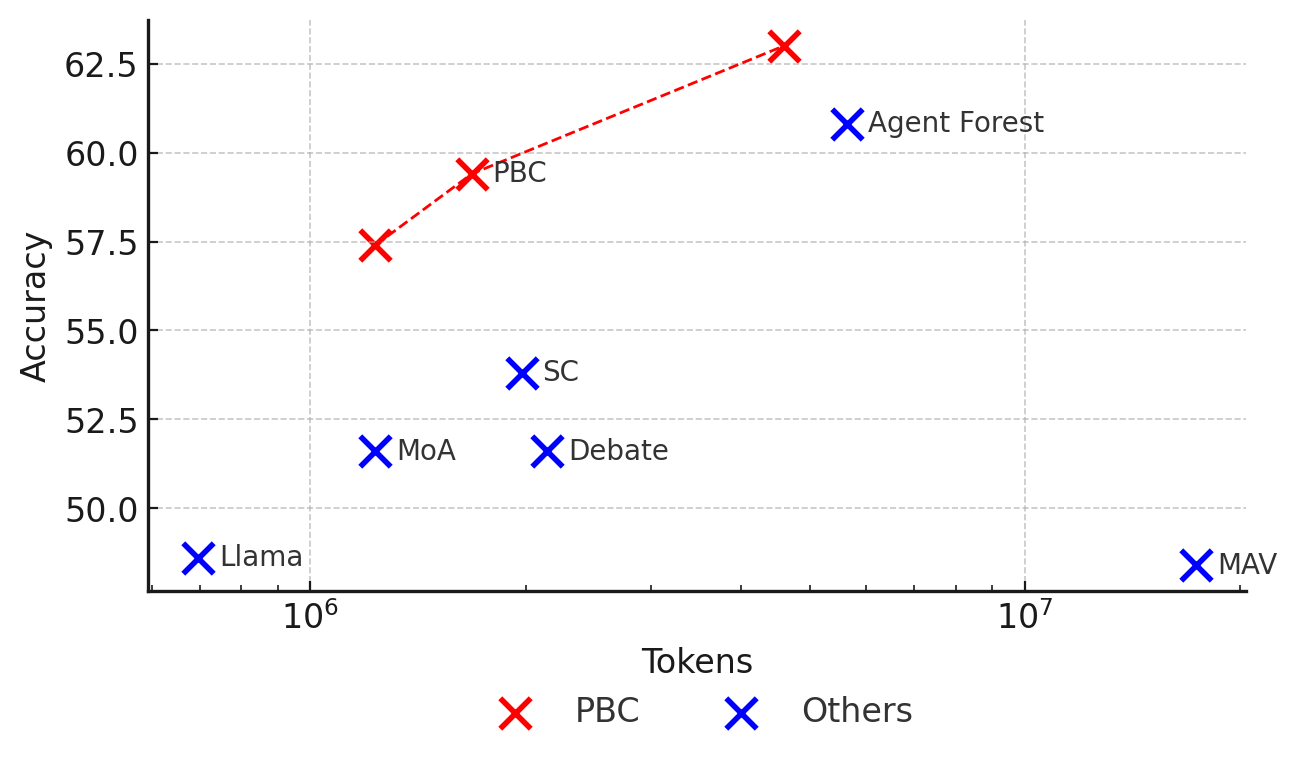
\includegraphics[width=0.8\linewidth]{Figures/Scatter_v1.png}
% \caption{\textbf{Token usage versus accuracy.} on the \textsc{MATH} dataset. Red markers denote the performance of our Protocol-based composition (\NAME{}) method built from three small models.}
% \label{fig:token-accuracy}
% \end{figure}

% For years, the path to more capable Large Language Models (LLMs) has been to relentlessly increase model parameters and data volume, resulting in models with trillions of parameters. Yet, the long-term sustainability of this scaling-first strategy is now in question. It faces two critical constraints: the prohibitive cost of computation and the finite supply of high-quality text data. With these bottlenecks, the returns from scaling are diminishing.

% At the same time, there has also been a surge of small-sized models in the range of a few billion to a few dozen billion parameters. These models are not state-of-the-art in terms of performance, but they offer much lower inference costs compared with the largest frontier systems. Moreover, different models also bring different capabilities.

Recent years have witnessed a surge of small-sized language models (SLMs) containing billions to tens of billions of parameters~\citep{wang2024comprehensivesurveysmalllanguage, javaheripi2023phi, guo2025deepseek, allal2025smollm2}. While these models may underperform state-of-the-art frontier language models, which usually contain hundreds of billions to trillions of parameters, on any given query, they offer substantially lower inference costs, are more affordable to train and finetune, and allow edge deployment due to their small size~\citep{belcak2025small}.  
Meanwhile, frontier models have reached trillion-parameter scales where further increases in size and training data yield diminishing returns. This mirrors a well-known challenge in computer architecture two decades ago: when enlarging single CPU cores no longer delivered proportional performance gains, computer architects turned to designing multi-core processors, where multiple smaller cores working together enabled sustained improvements.  This parallel suggests that combining multiple SLMs could offer a promising alternative to scaling ever-larger frontier models.


% This mirrors a well-known challenge in computer architecture two decades ago: when enlarging single CPU cores no longer delivered proportional performance gains, computer architects turned to designing multi-core processors, where multiple smaller cores working together enabled sustained improvements. 

% This parallel suggests that combining multiple SLMs could offer a promising alternative to scaling ever-larger frontier models. %This raises the question: would the field benefit more from an analogous architectural transition, shifting focus from developing increasingly large frontier models to optimizing ensembles of heterogeneous SLMs?%

% \cw{add GPT 5 into intro, add overall story on top}
% While scaling up model parameters and training data volume has historically been the primary route to stronger language models (LLMs), this strategy is increasingly constrained by hardware bottlenecks—such as limited GPU supply, a looming shortage of high-quality human-generated text, and diminishing performance gains at extreme scale. As a result, alternative approaches beyond brute-force scaling are becoming crucial for future progress.~\citep{scalinglaw,villalobos2024rundatalimitsllm,nellis2024nvidia}.

% At the same time, there has also been a surge of small-sized models in the range of a few billion to a few dozen billion parameters. These models are not state-of-the-art in terms of performance, but they offer much lower inference costs compared with the largest frontier systems. Moreover, different models also bring different capabilities, with their own strengths that make them valuable in specific contexts.

% Given these trends, a promising direction of research involves composing existing language models to create a more powerful ensemble. The central idea behind such compositional approaches is that different LLMs excel in different areas. By constructing a multi-model system that strategically integrates these individual strengths, the combined system can achieve performance levels exceeding those of any single model used alone, especially in more complex tasks~\citep{smit2024goingmadlookmultiagent,li2024agentsneed}. This method presents an opportunity to advance model capabilities without the significant costs and resources associated with continually scaling up a single model.

% Recently, several works have explored the composition of different language models. However, these approaches have predominantly focused on ensembles of state-of-the-art LLMs, which typically consist of models with tens to hundreds of billions of parameters. The composition in these frameworks is often realized through communication between the models. Given that these large models already possess strong individual capabilities and a high degree of instruction-following proficiency, they can collaborate effectively. In contrast, these works generally do not discuss the application of such compositional methods to smaller models—those in the few to tens of billions of parameters range. Furthermore, our preliminary investigations suggest that directly porting these existing techniques to smaller-scale models often fails to produce the desired performance gains.


%One line of work relies on router-based systems, where an auxiliary model or heuristic directs each query to the most appropriate LLM (\cite{openai_gpt5_2025, ong2024routellm, yue2025masrouter})). While effective, these methods typically require training or maintaining specialized routing models, which constrains their applicability in many scenarios and makes them less relevant for our setting.

Recent works have explored orchestrating multiple LLMs (e.g., GPT-3.5 and GPT-4o), combining them into one system to process an input collaboratively. Representative approaches include Mixture-of-Agent~\citep{wang2024mixtureofagentsenhanceslargelanguage}, LLM-Debate~\citep{du2023improvingfactualityreasoninglanguage}, and Multi-Agent Verification~\citep{lifshitz2025multiagentverificationscalingtesttime}. These approaches share a key assumption: that models possess strong reasoning and deliberation abilities, so that interaction through natural language can reliably correct mistakes. However, when applied to SLMs, this assumption no longer holds. Our study finds that \emph{such discussion-based orchestration often fails to improve performance for SLMs}, and in some cases even reduces accuracy by over 5\%. Instead of correcting mistakes, SLMs tend to fall into groupthink during interaction, amplifying errors rather than mitigating them. The assumptions that language models can correct each other's answers behind existing orchestration methods do not hold for SLMs~\citep{Taubenfeld_2024,huang2024largelanguagemodelsselfcorrect,liu2023lostmiddlelanguagemodels}. 


% Several recent works have explored combining different LLMs (such as GPT-3.5 and GPT-4) to improve model performance 
%  via structured discussion frameworks, where multiple LLMs interact to verify and refine each other’s answers (\cite{wang2024mixtureofagentsenhanceslargelanguage, pitre2025consensagent, du2023improvingfactualityreasoninglanguage}). For example, LLM-debate \citep{du2023improvingfactualityreasoninglanguage} proposes that model instances first produce individual responses and then engage in deliberation to converge on a common answer. These approaches heavily on models’ ability to engage in effective deliberation -- a capability that, as we analyze, remains limited in small-sized models. 

%For instance, OpenAI's latest model as of August 2025, GPT-5, consists of multiple language models; \citep{du2023improvingfactualityreasoninglanguage} proposed LLM-debate, an approach to improve language responses by having multiple language model instances individually propose and jointly debate their responses to arrive at a common answer.%


%Besides, SLMs often show complementary strengths, with each excelling on particular types of queries~\citep{ong2025routellmlearningroutellms}. Such heterogeneity may provide an advantage of combining multiple SLMs for inference. 


%Our analysis indicates that the ineffectiveness of these existing discussion-based methods in small size models stems from the weak cognitive abilities of SLMs. SLMs are weak in abilities such as reflection, verification, and distinguishing right from wrong when given a mixed answer. As a result, they cannot effectively learn from other language models. Our experimental results show that a debate between such small models usually leads to amplifying the wrong answer rather than finding the right one. Additionally, existing works on discussion-based methods often focus on proposing an architecture and demonstrating a prototype. However, they rarely address how such architectures can be easily adapted or improved across different domains.

% On the other hand, small-sized language models are also weak in their long-context ability. They struggle to effectively process the dynamic discussion among models.For some small-sized models, the context easily exceeds max allowed when using them to discuss with each other. Consequently, they have to rely on a fixed, pre-written prompt, which hinders them from eliciting their heterogeneous abilities.

% In this work, we propose \textbf{\NAME{}}, a multi-model architecture for effectively orchestrating SLMs while avoiding explicit text exchanges between models. Our key insight is that while prior discussion-based methods assume models possess complementary abilities and can learn through text communication, small-sized models actually fail in this paradigm, where text communication amplifies rather than corrects errors. \NAME{} leverages model heterogeneity by selecting outputs based on confidence scores without any model training. 

To address this issue, we propose \textbf{\NAME{}}, a multi-model architecture for effectively orchestrating SLMs while avoiding explicit text exchanges between models. Our key insight is that \NAME{} leverages complementary abilities from different models by selecting outputs based on confidence scores without any model training.


% To address this challenge, we introduce \textbf{\NAME{}}, a multi-model architecture that effectively coordinates multiple SLM for enhanced reasoning. Unlike prior approaches that rely on explicit discussions between models, \NAME{} estimates each model’s confidence using simple rules, without requiring inter-model text exchange. The system then selects the final output based on the confidence of models.


\begin{wrapfigure}{r}{0.5\linewidth}
  \centering
  \vspace{-5pt}
  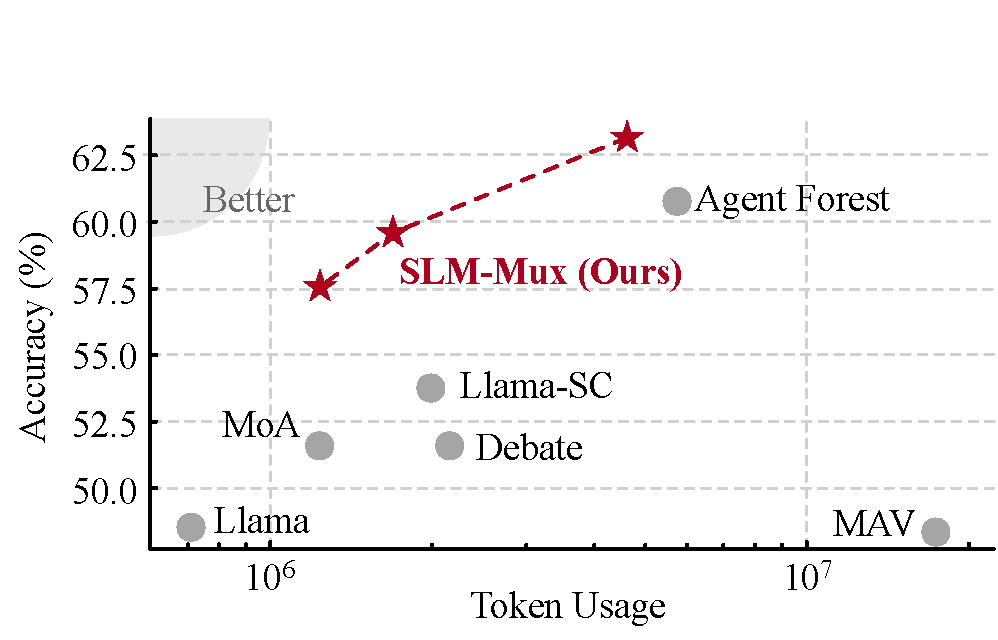
\includegraphics[width=\linewidth]{Figures/scatter_v3.pdf}
  \vspace{-15pt}
  \caption{\small \textbf{Head-to-Head Comparison of \NAME{} with Other Methods.} \NAME{} outperforms existing methods such as Self-Consistency (SC)~\citep{wang2023selfconsistencyimproveschainthought}, Mixture-of-Agents (MoA)~\citep{wang2024mixtureofagentsenhanceslargelanguage}, LLM-Debate~\citep{du2023improvingfactualityreasoninglanguage}, Multi-Agent Verification (MAV)~\citep{lifshitz2025multiagentverificationscalingtesttime}, and Agent Forest~\citep{li2024agentsneed}. Results reported on \textsc{MATH} dataset with SLMs.}
  \label{fig:token-accuracy}
  \vspace{-20pt}
\end{wrapfigure}

% After we have the \NAME{}, the next question emerges: with dozens of SLMs now available, we
% have access to a large model pool.  Since it is not feasible to invoke every SLM in the \NAME{}
% architecture for every given query, it is worth investigating whether there is an optimal strategy for
% selecting a limited subset of models for each task. On the other hand, model selection quality may impact the performance of \NAME{}.  For example, as shown in Figure~\ref{fig:motivation-search}, the two models on the left have no complementary capabilities. Llama 3.2 3B offers no advantage in every subject: for most (if not all) MATH questions, if Qwen 2.5 7B cannot solve them, neither can Llama 3.2 3B. In this case, combining them provides no benefit. However, the models on the right show complementary strengths: Mistral Small 24B scores higher in some subjects, and Qwen 2.5 7B does better in others. In this case, when Qwen 2.5 7B cannot answer a question, Mistral Small 24B may succeed.

After introducing \NAME{}, another question arises: which models should be orchestrated together? Not all combinations are effective -- if one model is weaker across all dimensions, it provides no benefit when paired with a stronger one. In contrast, combining models with complementary strengths (e.g., one stronger in algebra, another in geometry) allows the system to succeed where a single model would fail.

To address this, we develop a \textbf{model selection search strategy} for \NAME{}, which systematically evaluates and identifies model subsets with complementary strengths. By maximizing union accuracy while penalizing overconfident contradictions, the search procedure finds the most suitable models for a given model budget. 

In addition, we explore \textbf{compute scaling strategies} for the selected model ensembles to further enhance performance. By adjusting the number of models and samples at inference time, we further boost performance and identify practical sweet spots in the accuracy-compute tradeoff.


% We further develop an optimization strategy for model selection within the \NAME{} framework. Our method systematically identifies model combinations that maximize complementarity among small-sized LLMs, enabling us to achieve higher accuracy with minimal computational overhead by using only two or three models. This principled selection process ensures optimal performance while maintaining the efficiency advantages of SLMs.

% Second, to tackle the challenge of eliciting heterogeneous abilities with fixed prompts, we propose an inference-time prompt tuning method. This method specializes the prompt for each model to activate its unique strengths for a given query. By ensuring the models provide complementary abilities, the overall accuracy of the ensemble is significantly improved.

% second, we proposed a method to optimize \NAME{}. We  propose an method to select models based on their heterogeneity and maximize their heterogeneity between small-sized LLMs. 

Our experiments demonstrate significant improvements across multiple benchmarks. By combining only two SLMs, we achieve accuracy improvements of up to 6.7\% on MATH, 5.7\% on GPQA, and 4.8\% on GSM8K, compared to the best-performing single SLMs in the system. Our method consistently outperforms existing discussion-based approaches for SLMs, with gains of up to 13.4\% on MATH, 8.8\% on GPQA, and 7.0\% on GSM8K. Most importantly,  with just two SLMs, \NAME{}  outperforms Qwen 2.5 72B on GPQA and GSM, and matches its performance on MATH.

% \cw{Problem formulation: how to find a good performing SLM ensemble? }

Finally, we complement these empirical findings with theoretical and experimental analyses. Our approach shows superiority in multiple scenarios compared with previous methods (Figure \ref{fig:token-accuracy}). 

Our main contributions are as follows:
% :
% \begin{itemize}
% \begin{itemize}[leftmargin=2em, nosep]
% \item[{\bf i)}] We revisit the problem of multi-model composition with small-sized LLMs, and show that limited cognitive ability is a key factor underlying the failure of prior discussion-based methods.
% 
% \item[{\bf i)}] We propose Protocol-Based Composition (\NAME{}), a novel architecture that improves the compositional performance of small-sized models, achieving more accurate and efficient ensembles compared to prior approaches.
% 
% \item[{\bf i)}]
\textbf{ (i) We identify a fundamental limitation of existing orchestration methods:} Through systematic evaluation, we demonstrate that existing discussion-based methods, which show consistent improvements for frontier LLMs, actually harm performance when applied to SLMs. This counterintuitive finding challenges the assumption that orchestration methods transfer across model scales and reveals the need for SLM-specific method.
% 
% 
% \item[{\bf ii)}] We develop a model selection optimization technique that further improves the effectiveness of the proposed \NAME{} framework by enabling more principled and accurate selection of models.
% 
% 
% \item[{\bf ii)}] 
\textbf{(ii) We propose \NAME{}}, a novel multi-model architecture designed specifically for SLMs that avoids the error amplification problems of discussion-based methods. \NAME{}{} achieves consistent gains across multiple benchmarks (MATH, GPQA, GSM8K) and significantly outperforms existing discussion-based methods by large margins (up to 11.6\% on MATH).
% 
% 
% \item[{\bf iii)}] We demonstrate that our method significantly improves the performance of SLMs, achieving consistent gains across multiple benchmarks (MATH, GPQA, GSM8K) and outperforming both discussion-based multi-model composition architectures by a large margin.
% 
% \item[{\bf iii)}] 
\textbf{(iii) We develop principled optimization strategies} for the \NAME{}, including model selection search that identifies complementary model selections and compute scaling strategies, further boosting performance while maintaining efficiency.
% 
% 
% \cw{TODO architecture definition; change into architecture}

% \item We conduct extensive ablation studies and theoretical analyses to demonstrate the effectiveness of our proposed methods.
% \end{itemize}

% The remainder of this paper is structured as follows. Section~\ref{sect:related} reviews related work. Section~\ref{sect:failure} analyzes the limitations of existing discussion-based approaches. Section~\ref{sect:method} presents our proposed protocol-based composition framework and its optimizations. Section~\ref{sect:experiment} reports experimental results, while Section~\ref{sect:analysis} provides theoretical and ablation analyses. Finally, Section~\ref{sect:conclusion} concludes the paper and outlines future directions.

 
% \cw{new paper outline intro, related, method 1 limitation, method 2 composition, method 3 optimization, experiment, analyze 1 theory, analyze 2 ablation study}

 

% One promising alternative to address these constraints is compositional language models, which leverage existing LLMs more effectively by orchestrating them in structured workflows. The central idea behind compositional language models is that different LLMs excel in different areas. By constructing a multi-model system that strategically integrates these individual strengths, the combined system can achieve performance levels exceeding those of any single model used alone, especially in more complex tasks~\citep{smit2024goingmadlookmultiagent,li2024agentsneed}.

% For instance, multiple models can iteratively debate and critique each other's proposed solutions to resolve disagreements and enhance accuracy~\citep{du2023improvingfactualityreasoninglanguage}; responses from diverse LLMs can be integrated to generate higher-quality, more useful answers~\citep{wang2024mixtureofagentsenhanceslargelanguage}; or several models may independently evaluate candidate answers and collectively select the best response, thus improving mathematical accuracy~\citep{lifshitz2025multiagentverificationscalingtesttime}. 

% However, existing composition methods generally rely on repeated calling advanced, state-of-the-art language models, each requiring costly API calls. Given that these models are already resource-intensive individually, orchestrating several of them improves the overall expense significantly compared to employing just a single model directly to generate an answer~\citep{wang2024rethinkingboundsllmreasoning,gandhi2025budgetmlagentcosteffectivellmmultiagent}. As a result, these methods are often expensive. Exisiting works don't explore composition of small models.

% However, existing compositional methods typically involve repeated API calls to advanced, state-of-the-art LLMs, each call incurring significant computational cost. Because each of these models individually already consumes substantial resources, combining multiple models can greatly amplify the overall cost compared to simply using a single model~\citep{wang2024rethinkingboundsllmreasoning,gandhi2025budgetmlagentcosteffectivellmmultiagent}. As a result, current methods become prohibitively expensive. Furthermore, prior research has generally overlooked exploring compositional approaches using smaller-scale, less costly models.

% \begin{wrapfigure}{r}{0.5\linewidth}
%   \centering
%   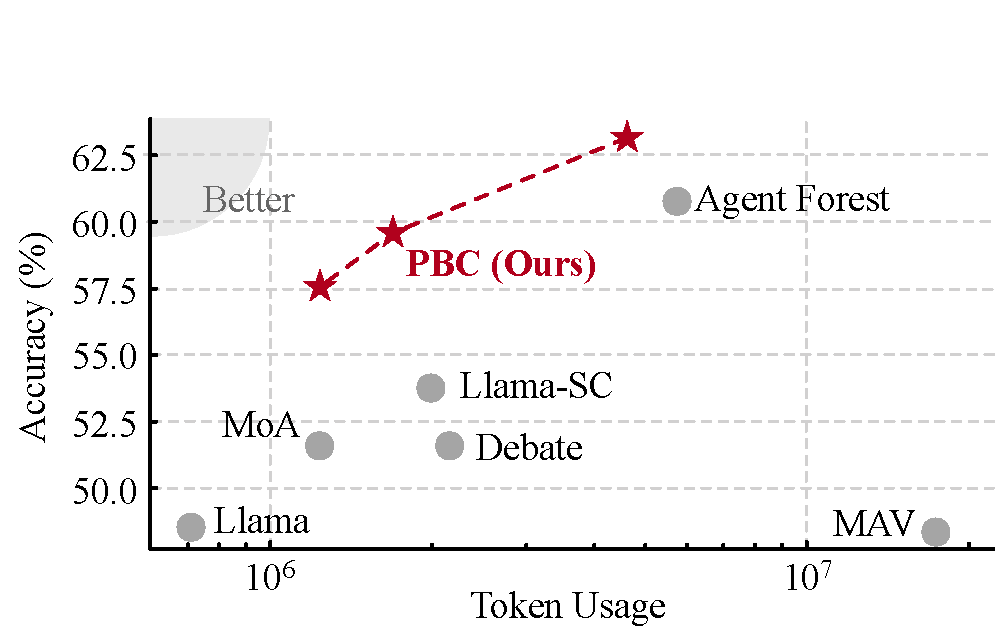
\includegraphics[width=\linewidth]{Figures/scatter_v2.pdf}
%   \vspace{-15pt}
%   \caption{\small \textbf{Protocol Based composition.} We present Protocol-based composition (\NAME{}), a new method to combine language models together which outperforms existing methods such as Self-Consistency (SC)~\citep{wang2023selfconsistencyimproveschainthought}, Mixture-of-Agents (MoA)~\citep{wang2024mixtureofagentsenhanceslargelanguage}, LLM-Debate~\citep{du2023improvingfactualityreasoninglanguage}, Multi-Agent Verification (MAV)~\citep{lifshitz2025multiagentverificationscalingtesttime}, and Agent Forest~\citep{li2024agentsneed}. Results reported on the \textsc{MATH} dataset with smaller-scale LLMs. }
%   \label{fig:token-accuracy}
%   \vspace{-10pt}
% \end{wrapfigure}

% Motivated by these observations, we explore whether it is possible to design a compositional method using smaller-scale, more economically friendly language models that can achieve similarly impressive performance improvements as those seen in larger-model systems, but at a lower cost. However, when directly applying existing compositional methods to smaller-scale models, we observed that the effectiveness of these methods is significantly reduced. This indicates that simply reusing current methods isn't sufficient—new approaches specifically designed for smaller-scale, economically friendly models are necessary.

% % Motivated by these cost and efficiency challenges, we investigate whether compositional language models constructed from smaller-scale, less resource-intensive models can achieve performance gains comparable to systems utilizing larger models. However, when directly applying smaller models within existing compositional methods, we observe a significant degradation in performance. Developing compositional methods specifically effective for smaller-scale models is not a straightforward task.

% % Although directly applying existing compositional methods to smaller language models usually leads to performance degradation, this issue is not insurmountable. Upon investigation, we attribute this decline primarily to two factors: superficial interactions between models and intrinsic capability limitations of smaller models themselves. Existing methods typically rely on sophisticated prompting techniques to facilitate interactions and aggregation of responses. However, these prompt-based interactions prove unstable and problematic for smaller models, hindering enhancement through interaction between models. Nonetheless, smaller models hold substantial compositional potential; we show that, theoretically, even three weak models (with accuracy <56\% on MATH~\citep{hendrycks2021measuringmathematicalproblemsolving} dataset) could significantly improve combined accuracy (64\%) if collected responses were perfectly selected. Motivated by this observation, we explore alternative compositional methods specifically tailored for smaller-scale models, proposing Protocol-based composition (\NAME{}) methods as a potentially more stable and effective alternative for smaller-scale models. Using our approach, we substantially improve the accuracy of smaller models, increasing their performance from below 56\% to approximately 63\%, closely approaching the theoretical upper limit.

% To understand why this performance gap arises, we analyzed the interactions among smaller-scale models. We found two main issues limiting their effectiveness: superficial interactions between models, and inherent capability constraints of smaller-scale models themselves. Existing compositional methods depend heavily on sophisticated prompting techniques, which are often problematic and ineffective for smaller-scale models. Despite these limitations, smaller-scale models still hold significant compositional potential. Our analysis shows that combining three relatively weak models—each with an average accuracy of around 46\% on the MATH dataset~\citep{hendrycks2021measuringmathematicalproblemsolving}—can theoretically achieve a combined accuracy of approximately 64\%, assuming optimal selection among their outputs. Inspired by this insight, we propose Protocol-based composition (\NAME{}), a compositional approach specifically tailored for smaller-scale models that relies on structured rules rather than fragile prompt-based interactions. Using \NAME{}, we successfully improved accuracy from below 56\% up to approximately 63\%, closely approaching the theoretical limit.


% More excitingly, integrating our \NAME{} method with existing compositional methods significantly reduces token usage by up to 6.26$\times$: we introduce a dynamic routing mechanism to select between \NAME{} and existing methods based on input characteristics. This efficiency gain arises because \NAME{} employs simpler, rule-based interactions rather than relying on complex prompt-driven interactions between models. As illustrated in Figure~\ref{fig:token-accuracy},  \NAME{} significantly outperforms prior methods that combine multiple language models together.

% Our contributions are summarized as follows:

% \begin{itemize}[leftmargin=2em]
%     \item We analyze and identify two main reasons why existing compositional methods struggle when directly applied to smaller-scale language models: superficial interactions between models and intrinsic capability limitations of individual smaller-scale models.
    
%     \item We propose Protocol-based composition (\NAME{}), a novel method for composing smaller-scale LLMs. Unlike conventional approaches that rely on sophisticated prompts, \NAME{} employs a simple rule-based approach. Our method significantly enhances the accuracy of smaller-scale models.
    
%     \item We introduce a dynamic routing mechanism that adaptively selects between our \NAME{} method and existing compositional methods utilizing state-of-the-art LLMs, based on input characteristics. Our method significantly reduces token usage of Multi-Agent Verification~\citep{lifshitz2025multiagentverificationscalingtesttime} method by 6.26$\times$, while maintaining comparable accuracy levels.
% \end{itemize}

%  The remainder of the paper is organized as follows: In Section~\ref{sect:related}, we discuss related work, including existing approaches to inference-time computation and compositional language models. Section~\ref{sect:method} presents our analysis on the reasons for performance degradation in smaller-scale models and introduces our proposed method. Experimental results are detailed in Section~\ref{sect:experiment}, followed by the conclusion in Section~\ref{sect:conclusion}.
 


% \vspace{-5pt}
\section{Related Work}
% \vspace{-3pt}
\label{sect:related}
% \paragraph{Inference-Time Compute Techniques:} Inference-time compute involves using extra computational resources during inference time to improve the accuracy of language models.~\citep{snell2024scalingllmtesttimecompute,sumers2023cognitive,liu20251bllmsurpass405b,yang2025thinkingoptimalscalingtesttimecompute} For example, language models can produce intermediate outputs or reasoning steps before arriving at a final answer~\citep{wang2023selfconsistencyimproveschainthought,wei2023chainofthoughtpromptingelicitsreasoning}. Alternatively, compositional language model techniques compose multiple models at inference time to achieve better performance than a single model~\citep{li2024agentsneed,yin2024aggregationreasoninghierarchicalframework}.

% Producing intermediate outputs at inference time has been shown to significantly enhance smaller-scale models' performance~\citep{liu20251bllmsurpass405b}. However, existing research in compositional language models mostly focus on designing new methods using state-of-the-art LLMs~\citep{du2023improvingfactualityreasoninglanguage,khattab2023dspycompilingdeclarativelanguage,wu2023autogen}. However, whether smaller-scale models can benefit significantly from compositional methods remains an open question and is currently underexplored. Our work attempts to address this issue.

% \cw{TODO add a discussion based method definition}

% \paragraph{Compositional Language Models:} Compositional language models involve multiple language models working together to produce better results than a single model could achieve alone~\citep{jiang2023llmblenderensemblinglargelanguage,li2025rethinkingmixtureofagentsmixingdifferent,mitra2024distributedmixtureofagentsedgeinference}. By interacting and cooperating, these models combine their individual strengths through structured processes, including collaborative reasoning, critique, and verification, improving the quality of their final outputs~\citep{liang2024encouragingdivergentthinkinglarge,shinn2023reflexionlanguageagentsverbal,park2024ensemblinglargelanguagemodels,chen2025harnessingmultiplelargelanguage,khan2024debatingpersuasivellmsleads,gou2024criticlargelanguagemodels,mousavi2023ncriticsselfrefinementlargelanguage,gu2025surveyllmasajudge}. For example, LLM-Debate involves language models debating and critiquing each other to refine their final answers~\citep{du2023improvingfactualityreasoninglanguage}; Mixture-of-Agents synthesizes outputs from different models to produce comprehensive results~\citep{wang2024mixtureofagentsenhanceslargelanguage}; Multi-Agent Verification uses multiple models to independently evaluate candidate answers from different aspects and collectively select the best answer~\citep{lifshitz2025multiagentverificationscalingtesttime}. Figure~\ref{fig:comparison-methods} illustrates the workflow of these three methods. Despite the success of these methods, prior studies have primarily focused on composing frontier LLMs, while the composition of small-sized LLMs remains unexplored.

% Besides developing new frameworks, recent research has started optimizing existing compositional methods. Some studies focus on examining and optimizing model selection within these frameworks to improve their performance~\citep{li2025rethinkingmixtureofagentsmixingdifferent,chen2025optimizingmodelselectioncompound}. Other researchers try to enhance efficiency by improving the workflows or interaction designs of these methods. However, these efficiency improvements typically target specific methods rather than offering universally applicable solutions~\citep{li2024smoaimprovingmultiagentlarge,li2024improvingmultiagentdebatesparse,liu2024dynamicllmpoweredagentnetwork}.

\begin{figure}[t!]
    \centering
    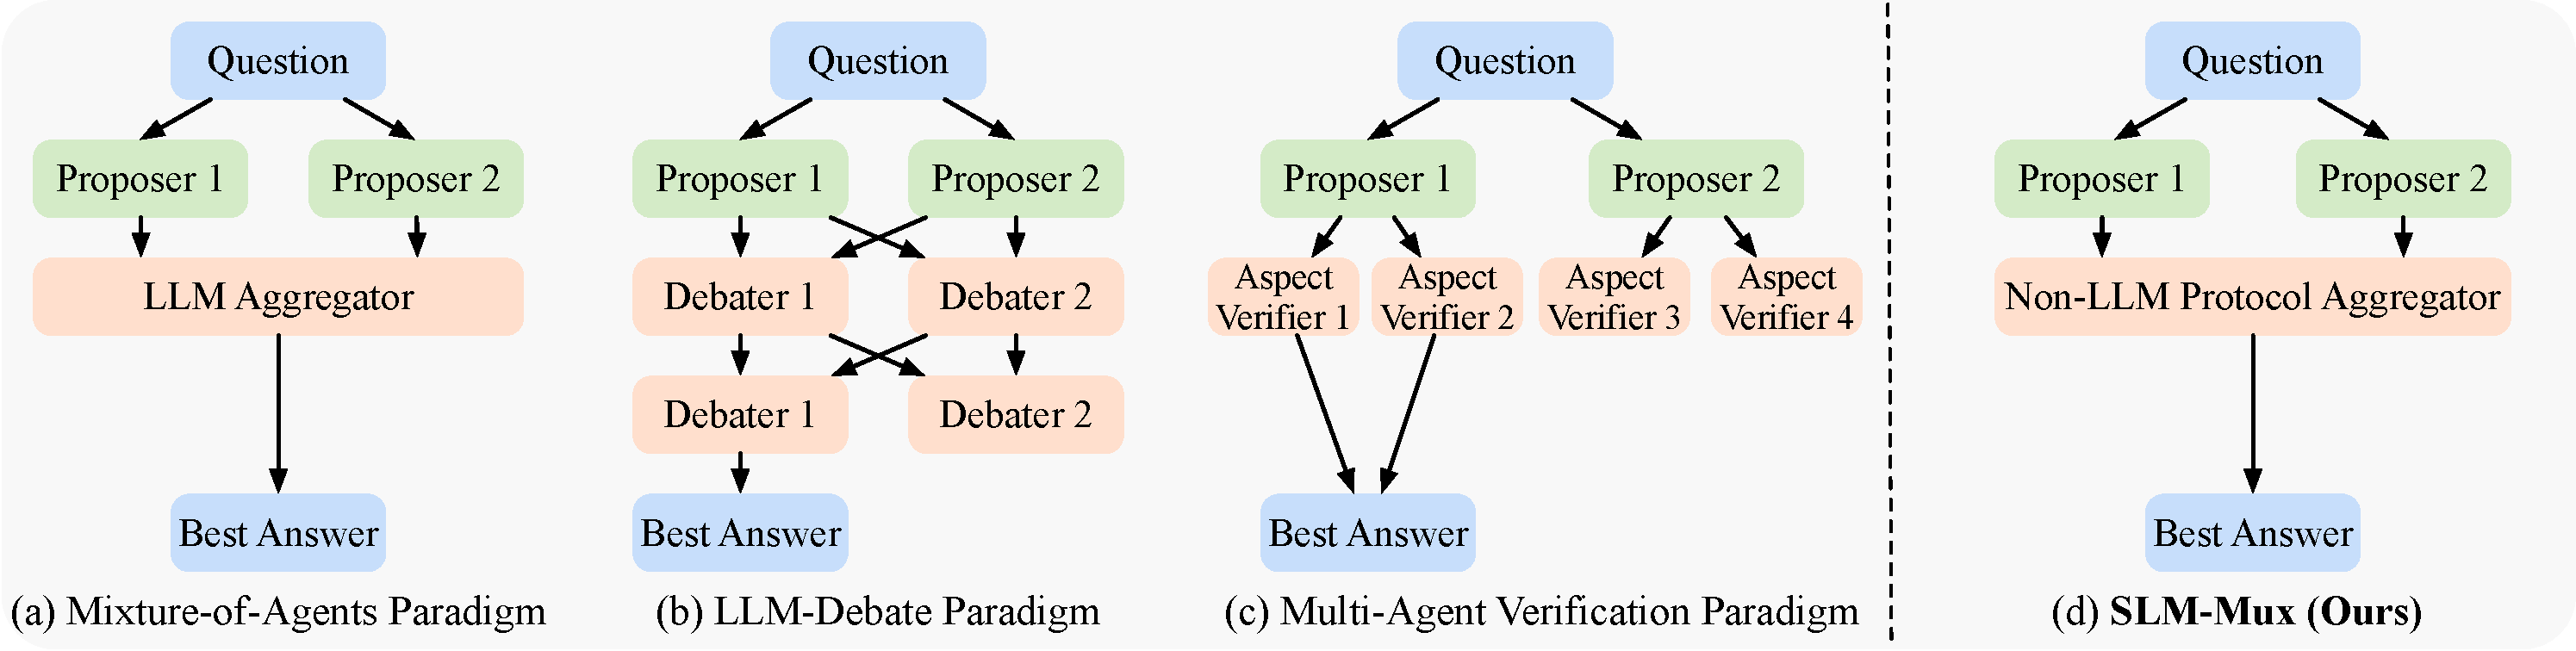
\includegraphics[width=\textwidth]{Figures/comparison_v3.pdf}
    \vspace{-10.5pt}
    \caption{\small \textbf{Comparing SLM-Mux (Ours) with Existing LLM Orchestration Methods.} (a) Mixture-of-Agents, (b) LLM-Debate, (c) Multi-Agent Verification, (d) SLM-Mux (Ours).}
    
    \label{fig:comparison-methods}
    % \vspace{-5pt}
\end{figure}

% \paragraph{Language Models Architectures Optimization}
% A growing body of work has explored engineering and orchestrating multiple LLMs into a single inference-time workflow. On the framework side, several systems allow users to design customized architectures~\citep{chen2023agentversefacilitatingmultiagentcollaboration,hong2024metagptmetaprogrammingmultiagent,shen2023hugginggptsolvingaitasks,li2023camelcommunicativeagentsmind}. For example, Autogen supports multi-agent conversation and tool integration~\citep{wu2023autogenenablingnextgenllm,schick2023toolformerlanguagemodelsteach}; and OpenAgents offers a deployable platform for data, web, and plugin-based agents~\citep{xie2023openagentsopenplatformlanguage}. 

% On the optimization side, prior work has focused on improving these compound LLM architectures, either by refining prompts or by searching for optimal workflows that guide LLMs to produce stronger outputs~\citep{khattab2023dspycompilingdeclarativelanguage,fernando2023promptbreederselfreferentialselfimprovementprompt,zhang2025aflowautomatingagenticworkflow,saadfalcon2025archonarchitecturesearchframework,opsahlong2024optimizinginstructionsdemonstrationsmultistage}. However, such approaches generally assume models with strong instruction-following abilities that are compatible with discussion-based frameworks. This assumption does not hold in our setting, which uses small-sized LLMs. Another line of work addresses model selection within compound LLM architectures~\citep{chen2025optimizingmodelselectioncompound,poon2025online}, but these approaches typically optimize only considering individual model accuracy without considering heterogeneity in model abilities. This limitation also makes them unsuitable for our setting.



% \paragraph{Test-time Scaling}
% Test-time scaling refers to methods that use extra computational resources during inference to boost model performance without retraining~\citep{snell2024scalingllmtesttimecompute,muennighoff2025s1simpletesttimescaling,zhang2025surveytesttimescalinglarge}. One line of work focuses on sampling multiple outputs from LLMs~\citep{chen2023universalselfconsistencylargelanguage,ichihara2025evaluationbestofnsamplingstrategies}. For example, self-consistency queries the model several times and uses the diversity of responses to estimate confidence, often improving accuracy~\citep{Trad_2025,thirukovalluru2024atomicselfconsistencybetterlong,chow2024inferenceawarefinetuningbestofnsampling}. However, most existing studies focus on a single model, whereas our work lies in the largely unexplored direction of combining the complementary strengths of multiple LLMs. 

% Another line of work encourages LLMs to spend more time reasoning before giving a final answer~\citep{wei2023chainofthoughtpromptingelicitsreasoning,yao2023treethoughtsdeliberateproblem,Besta_2024,dohan2022languagemodelcascades}. However, these approaches require further training of LLMs, which limits their flexibility across diverse use cases. In contrast, our method can directly utilize off-the-shelf models without additional training.

% However, test-time compute has limits. As the compute budget increases, performance eventually plateaus~\citep{dohan2022languagemodelcascades,chen2024llmcallsneedscaling}. The ceiling is determined by the capability of the underlying base model~\citep{chu2025ssrspeculativeparallelscaling,wu2025inferencescalinglawsempirical}. These limits motivate exploring more efficient and effective ways to compose multiple base LLMs at test time.

\paragraph{Discussion-based Orchestration Methods} We use discussion-based orchestration to refer to orchestration schemes where multiple LM instances exchange or evaluate natural-language messages—such as proposing answers, critiquing or debating, verifying from different aspects, and finally aggregating into one output. Representative approaches include Mixture-of-Agents~\citep{wang2024mixtureofagentsenhanceslargelanguage}, which uses a dedicated LLM to aggregate outputs from several models; LLM-Debate~\citep{du2023improvingfactualityreasoninglanguage}, where models critique and refine each other’s reasoning; and Multi-Agent Verification~\citep{lifshitz2025multiagentverificationscalingtesttime}, which assigns models to independently evaluate candidate solutions before selecting the final answer. These methods assume that participating models have sufficient reasoning ability to self-correct through interaction. Prior evaluations have been conducted on frontier LLMs, while their effectiveness for SLMs remains unstudied.

\looseness=-1
\paragraph{Optimization for Multi-LM Orchestration} Given these orchestration methods, some works study how to further improve their performance—e.g., how to select models to include, how to optimize prompts, or how to adapt the architecture for specific tasks~\citep{chen2023frugalgptuselargelanguage,ong2025routellmlearningroutellms,chen2024routerdcquerybasedrouterdual}. Prompt and workflow optimization methods~\citep{khattab2023dspycompilingdeclarativelanguage,opsahlong2024optimizinginstructionsdemonstrationsmultistage,saadfalcon2025archonarchitecturesearchframework, zhang2025aflowautomatingagenticworkflow} generally assume strong instruction-following ability, which makes them less effective for smaller models.

Another line of work is model selection for orchestration~\citep{chen2025optimizingmodelselectioncompound,poon2025online}. These methods often assume that models with higher standalone accuracy will yield stronger orchestrations. However, such strategies overlook conflicts among models: overconfident but incorrect predictions can dominate and suppress correct ones. Moreover, most selection criteria are not end-to-end—they evaluate models individually without directly assessing the performance of the orchestration itself. 

\paragraph{Test-time Scaling Strategies}
Test-time scaling refers to methods that improve performance by using additional computation during inference without retraining~\citep{snell2024scalingllmtesttimecompute,muennighoff2025s1simpletesttimescaling,zhang2025surveytesttimescalinglarge}. For a single model, a common approach is self-consistency~\citep{Trad_2025,thirukovalluru2024atomicselfconsistencybetterlong,chow2024inferenceawarefinetuningbestofnsampling}, where multiple samples are drawn and the majority answer is selected; accuracy typically improves as the number of samples increases. Extending this idea to multiple models, Agent Forest~\citep{li2024agentsneed} asks each model to produce one output and then applies majority voting over the pool of answers.

% \vspace{-5pt}
% \section{The Challenge of Composing Small Language Models}
% \vspace{-3pt}
% \label{sect:failure}
% Before presenting our methods in Section~\ref{sect:method}, we first compare composition architectures that invoke either SLMs (typically mid-performing) or frontier LLMs, in order to highlight the performance gap within prior discussion-based architectures. Specifically, we evaluate three discussion-based composition architectures: LLM-Debate~\citep{du2023improvingfactualityreasoninglanguage}, Mixture-of-Agents~\citep{wang2024mixtureofagentsenhanceslargelanguage}, and Multi-Agent Verification~\citep{lifshitz2025multiagentverificationscalingtesttime}. We use the same experimental settings for SLMs and frontier LLMs; we vary only the choice of models between a small-sized group and a frontier (often larger) group.

As shown in Figure~\ref{fig:small-large-accuracy}, discussion-based architectures generally outperform the single best-performing models in the frontier LLM group, achieving up to a 2\% increase in accuracy. However, when applied to SLMs, these discussion-based architectures fail to outperform the best single model in the composition, and even incur accuracy drops of up to 5.5\%. This performance gap is observed across all three methods and both benchmarks. This raises a central question: are existing discussion-based architectures truly suitable for SLMs?

% In this section, we conduct an thorough evaluation and analysis existing LLM combination methods. While existing LLM combination methods (such as LLM-debate, multi-agent verification) show good performance gain, they usually directly utilize frostier models such as GPT 3.5 and GPT 4. Given larger models usually have a better pretraining volume and cognitive ability, they usually benefit from discussing with each other. It is worth questioning that if these methods will still hold true under small models settings, where models have limited knowledge and generally weak cognitive ability.    

% As shown in Figure~\ref{fig:small-large-accuracy}, existing combination methods consistently yield superior performance for large-sized, frontier models, often outperforming any individual model. However, when applied to smaller-scale models, these methods fail to deliver gains over the strongest individual model, despite incurring substantial computational and token usage costs due to multiple model queries. Existing combination methods that is based on text communication between models are ineffective when using small-scaled, mediocre-performing language models.

% To analyze why this ineffectiveness happens, we further investigate into the failure cause of the methods.

% This observation underscores a key limitation: compositional methods that rely on iterative reasoning or multi-step interactions exhibit a strong dependency on the underlying model's capabilities. In the case of smaller-scale models, the additional rounds of reasoning do not lead to higher accuracy. Instead, accuracy often plateaus or even degrades, suggesting that interaction-based composition may not be suitable for resource-constrained or lower-capacity models.


\begin{figure}[htbp]
  \centering
  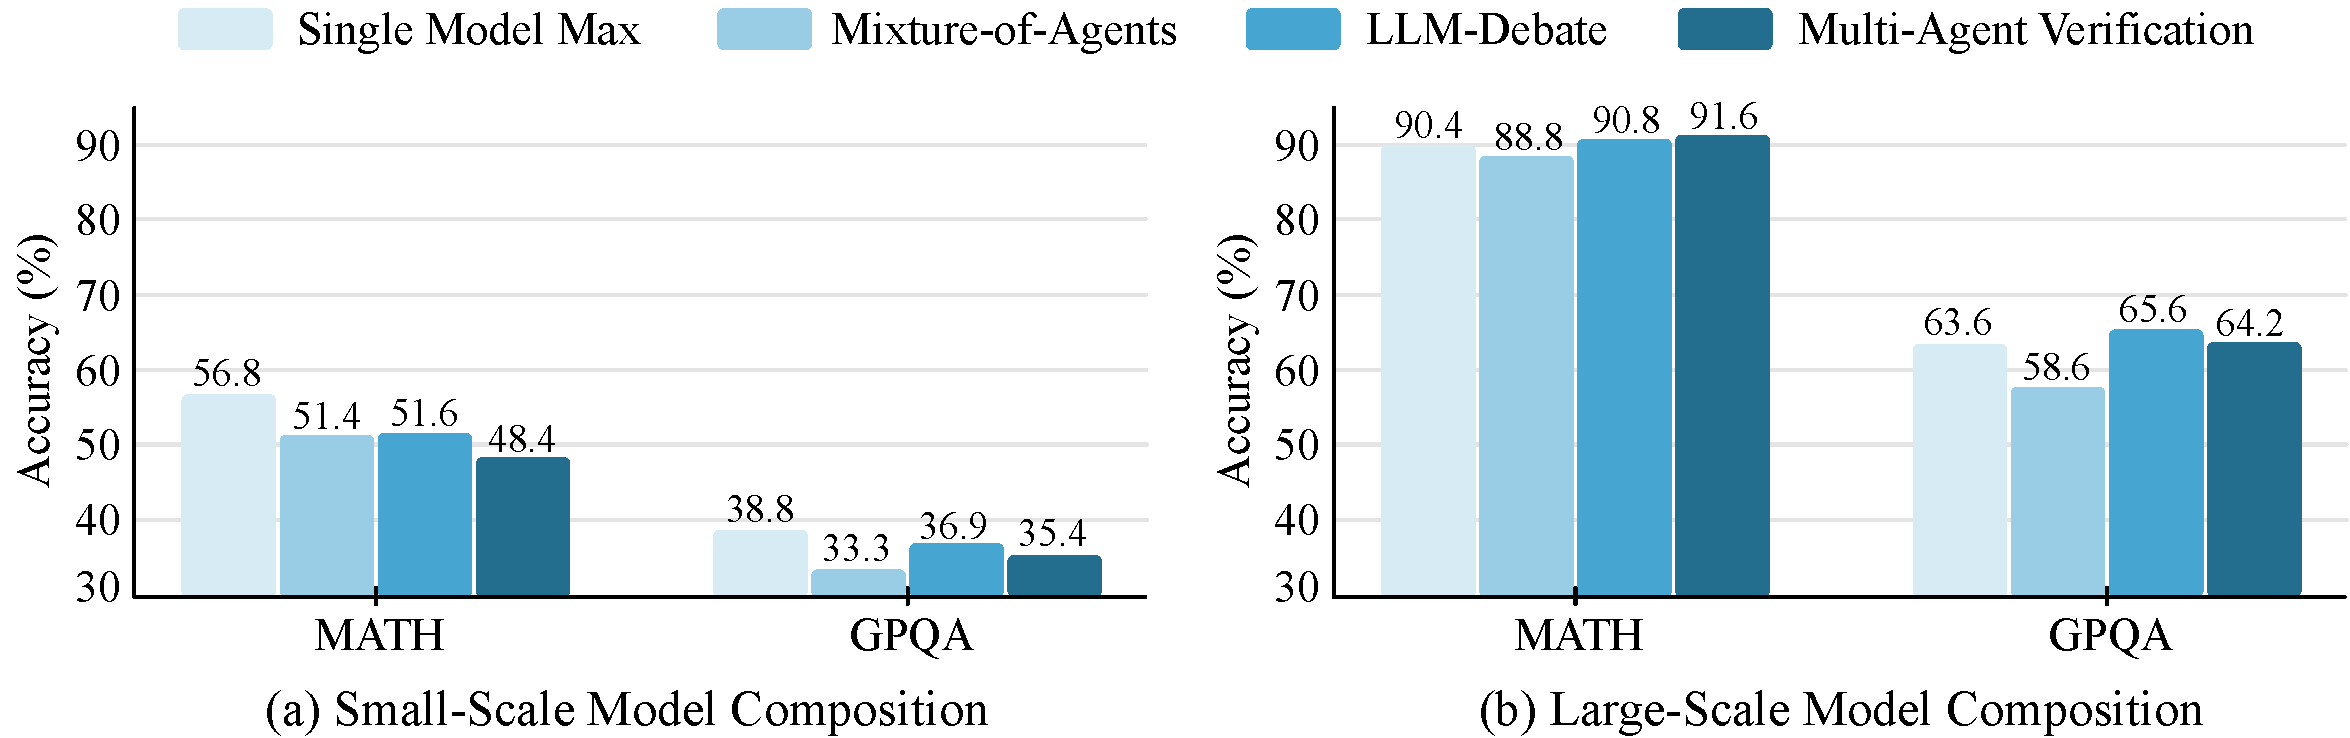
\includegraphics[width=0.9\linewidth]{Figures/Small-large-acc-light-blue_v2.pdf}
  \vspace{-8pt}
  \caption{\small \textbf{Comparison of discussion-based orchestration when invoking SLMs and LLMs.} We compare three compositional architectures (Mixture-of-Agents, LLM-Debate, and Verification) using (a) SLMs (Llama 3.1 8B, Mistral 8$\times$7B, Gemma 2 27B) and (b) frontier LLMs (DeepSeek V3, Gemini 2.0 Flash, GPT-4o) on the \textsc{MATH} and \textsc{GPQA} datasets. The baseline (\textit{Single-Model Max}) reflects the best performance of individual models. A composition is considered successful if it surpasses Single-Model Max.}\label{fig:small-large-accuracy}
  \vspace{-10pt}
\end{figure}


% To understand why compositional methods underperform with smaller language models, we conducted a detailed diagnostic analysis of representative failure cases using the LLM-Debate method~\cite{du2023improving}. Specifically, we examined dialogue transcripts from model interactions on the MATH dataset involving computationally efficient models (Mistral-8$\times$7B, LLaMA-3.1-8B, Gemma-2-27B). Our analysis revealed two overarching categories of failure:

To better understand this gap, we analyze the behavior of SLMs. Our findings highlight a key limitation: rather than correcting mistakes, discussion-based methods often amplify them. Our two observations support this claim: (1) when prompting an LLM to explain failures in the debate setting, we find that the discussions tend to reinforce incorrect reasoning rather than resolve it. (2) From a statistical perspective, we observe that SLMs tend to adopt the answer most recently presented in the context, rather than reviewing and reflecting on the entire discussion. More details of this analysis are presented in the Appendix.

Together, these observations suggest that existing discussion-based frameworks are ill-suited for SLMs. Their limited reasoning capacity necessitates a new composition architecture, which we will present in Section~\ref{sect:method}.


% \begin{figure}[t]
%   \centering
%   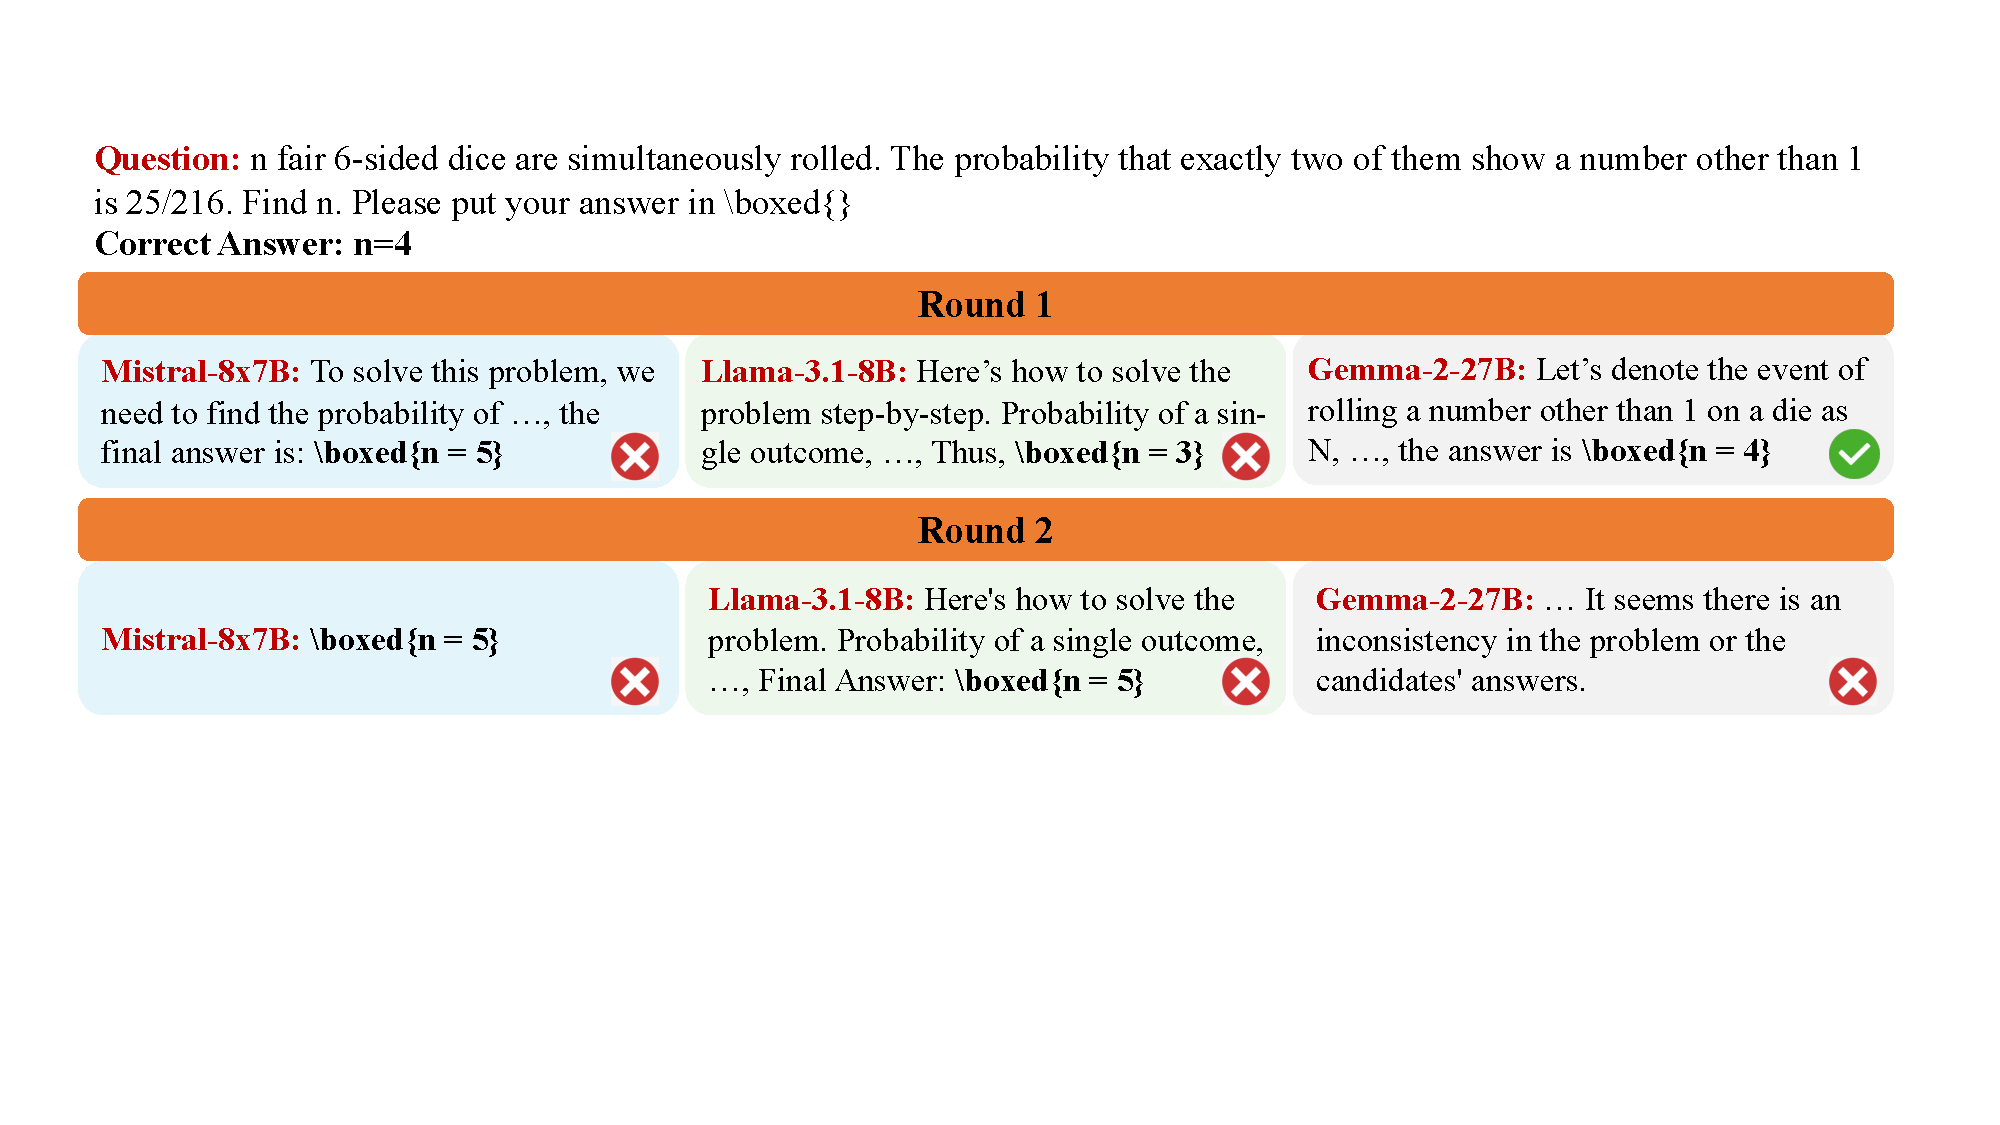
\includegraphics[width=\linewidth]{Figures/failure_case_interaction.pdf}
%   \vspace{-10pt}
%   \caption{\small \textbf{Illustration of Superficial Interactions.} A failure case illustrating ineffective interaction in a small-model debate setting. Model 1 simply repeated its previous answer without any additional reasoning.}
%   \vspace{-5pt}
%   \label{fig:fail-case}
% \end{figure}

% \paragraph{Superficial Interactions.} 
% A significant failure mode involves superficial engagement, which can manifest in various unproductive behaviors during debates. For instance, models sometimes simply repeat previous answers without genuine reconsideration or reflection, ignoring the debate's iterative nature and the expectation to refine their responses. Other models may merely critique perceived inconsistencies or errors in peer responses without contributing substantive new ideas or solutions. Occasionally, models revert to earlier solutions for verification without progressing further, failing to advance the discussion. Additionally, certain models may incorporate flawed elements from peer answers directly into their own revised solutions, unintentionally propagating errors rather than correcting them. These types of superficial and non-reflective interactions collectively undermine the intended dynamic and progressive nature of debate methodologies.

% Figure~\ref{fig:fail-case} illustrates a representative example of superficial engagement. In Round 1, three models respond to a probability problem involving dice rolls: Model 1 and Model 2 produce incorrect answers, while Model 3 identifies the correct solution. However, during Round 2, rather than engaging deeply with each other's reasoning as intended, Model 1 merely repeats its initial incorrect response without any further reasoning. Model 2, influenced negatively by Model 1, shifts from one incorrect answer to another without genuinely incorporating the correct insight from Model 3. Model 3, despite having provided the correct solution initially, deviates from the task in Round 2 by critiquing the inconsistencies of the other models rather than reaffirming or further elaborating its original correct response. This leads Model 3 to abandon its initial correct answer, demonstrating the superficial level of engagement that inhibits effective debate and knowledge integration among models.


% \paragraph{Intrinsic Capability Limitations.} 
% % Another important limitation is related to the intrinsic abilities of smaller models. This limitation does not seem to be related to the interactions between models, but rather because of their inherent limitations. For example, smaller models often have difficulty placing their answers exactly where we expect them, especially as the context grows longer. Additionally, all models sometimes struggle to identify the common error in their answers, even after debate.
% Another critical challenge arises from the inherent limitations of smaller language models, independent of their interactions with other agents. These limitations often manifest as difficulties in adhering to formatting expectations or in maintaining reasoning consistency, especially as prompt contexts grow longer. For instance, smaller models frequently misplace final answers or fail to follow explicitly specified output structures. Additionally, even after multiple rounds of debate, models often struggle to recognize and correct common reasoning errors, highlighting fundamental constraints in their self-correction capabilities.

% \begin{figure}[htbp]
%   \centering
%   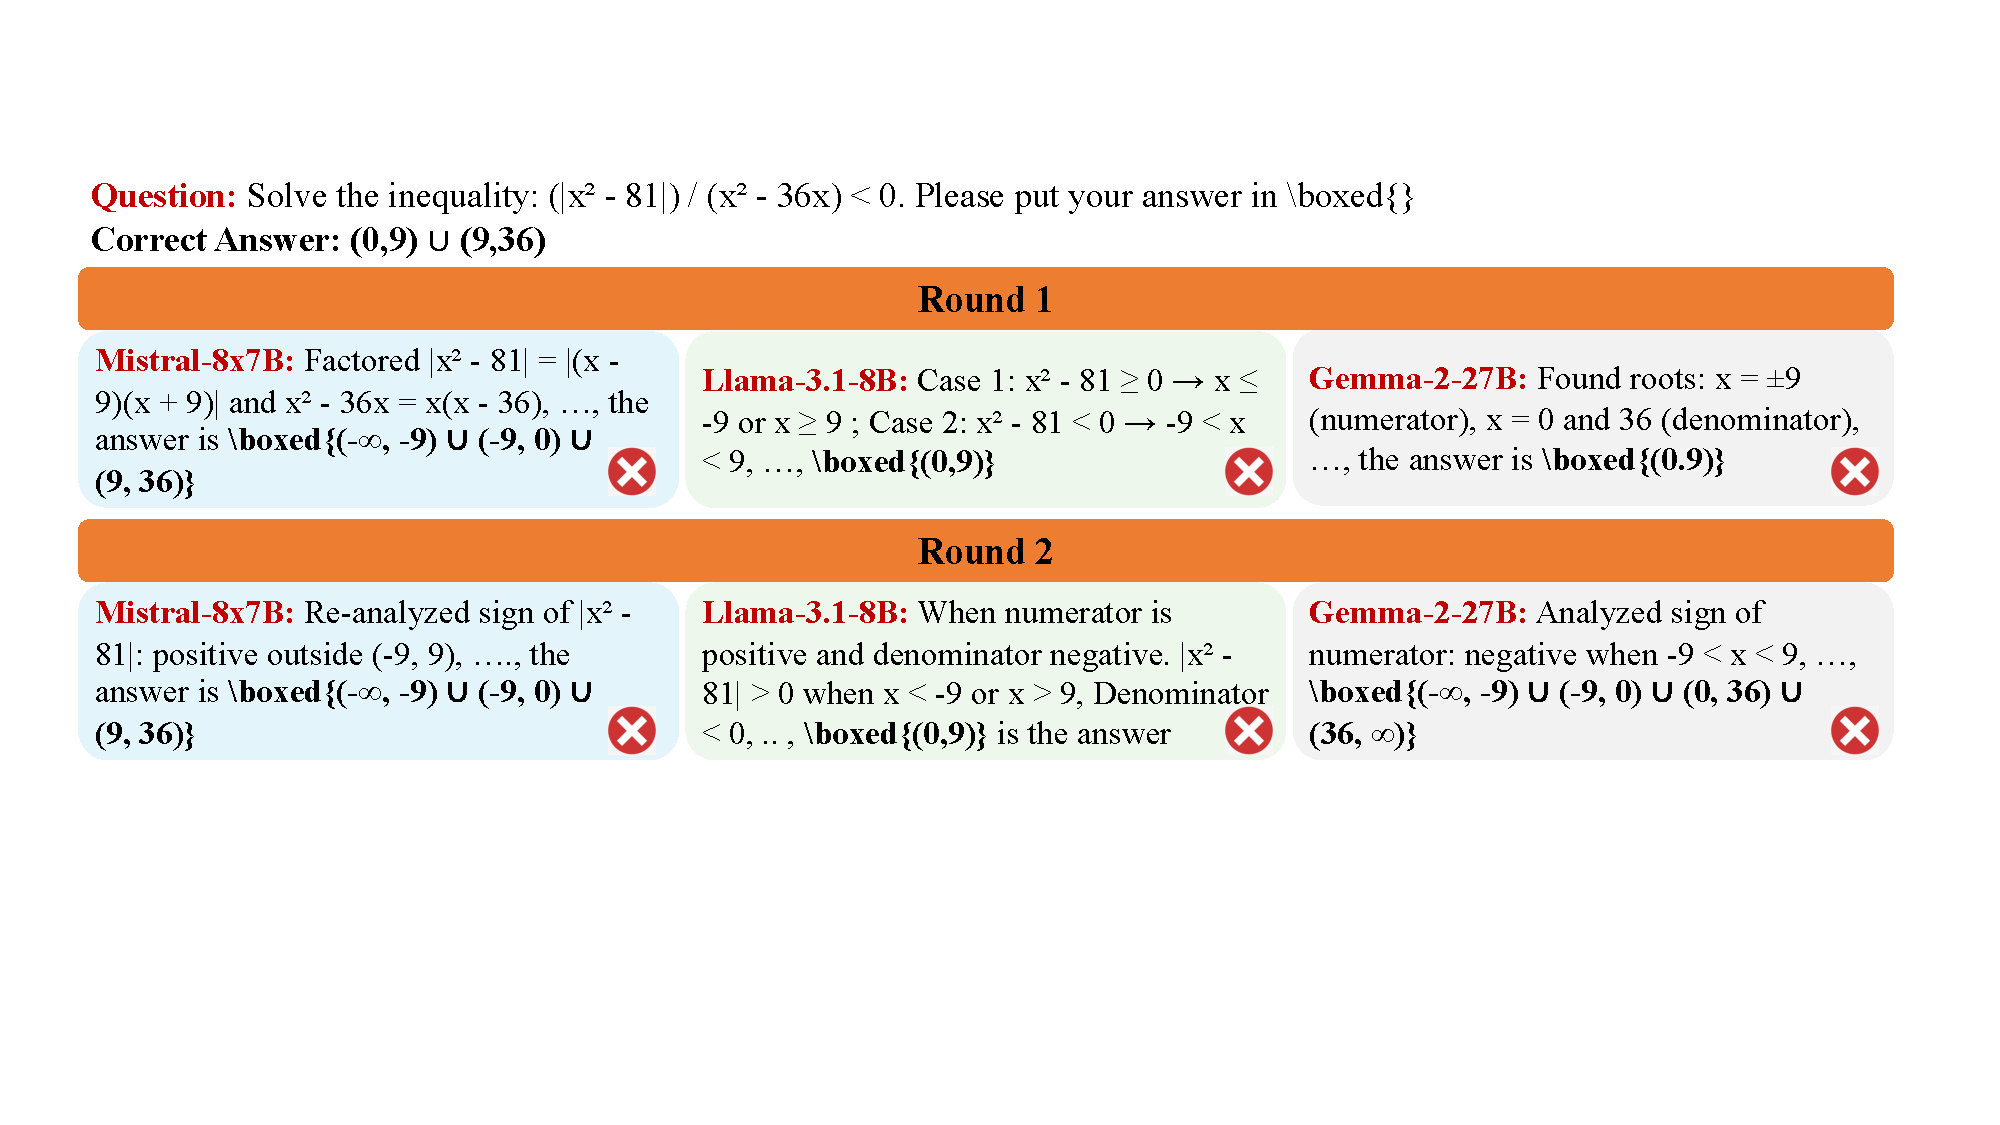
\includegraphics[width=\linewidth]{Figures/failure_case_model_capability.pdf}
%   \vspace{-10pt}
%   \caption{\small \textbf{Illustration of Intrinsic Capability Limitations.} A failure case illustrating an intrinsic capability limitation of the model. The model failed to correctly identify the conditions of the problem and did not place the solution in the prompt-specified location. For clarity and conciseness, we summarize the reasoning process.}
%   \label{fig:fail-case-2}
%   \vspace{-15pt}
% \end{figure}

% % Figure~\ref{fig:fail-case-2} illustrates an intrinsic capability limitation observed in small models. Specifically, in this example, the models failed to accurately determine the sign intervals of the numerator and denominator during the problem-solving process, leading to incorrect identification of the function's sign and thus incorrect solution intervals. All models fail to correct this mistake after the debate. Additionally, model 2 did not correctly place the final answer in the explicitly specified location, complicating the extraction of the solution. Although misplacement of answers might seem minor, such errors frequently occur and significantly impact the overall effectiveness of small-model compositions.

% Figure~\ref{fig:fail-case-2} presents an example of such intrinsic limitations. In this case, all models fail to correctly identify the sign intervals of the numerator and denominator, resulting in an incorrect determination of the function’s sign and solution intervals. Despite the opportunity for collaborative correction during debate, the error persists across all responses. Moreover, Model 2 fails to place the final answer in the designated location, making the solution harder to extract—an issue that, while seemingly minor, frequently undermines the practical utility of small-model outputs in compositional workflows.

% Interestingly, we observe that smaller models perform consistently well when responding directly to prompts. Although their answers are not always accurate, the errors typically stem from knowledge or reasoning limitations rather than misunderstandings of prompt structure or formatting. This contrast highlights that the core challenges lie not in instruction-following ability, but in the models’ limited capacity to handle complex reasoning tasks and participate effectively in multi-agent interactions.


% \vspace{-5pt}
\section{Methods}
% \vspace{-3pt}
\label{sect:method}
% \subsection{Overview}
% \label{subsec:method_overview}

% In this section, we introduce a new compositional architecture for orchestrating multiple SLMs and discuss its optimization. 


% Firstly, to address the challenge mentioned in Section~\ref{sect:failure}, we introduce a simple yet effective architecture that integrates models through a protocol-based mechanism (Section~\ref{sub:method-arch}). Based on this architecture, we introduce strategies to optimize \NAME{}{} from two directions: From the model perspective, we introduce model selection search to identify the most appropriate model to invoke within the \NAME{}{} (Section~\ref{sub:method-search}). From the test-time compute perspective, we explore optimal way compute scaling for the \NAME{}{} with searched model selections (Section~\ref{sec:scaling}). 

In this work, we set out to ask two critical questions: given a pool of available SLMs, how can we (i) orchestrate their outputs to achieve the best overall performance, and (ii) select an effective subset of models that maximizes accuracy?

To answer question (i), we present the \NAME{}{} (Section~\ref{sub:method-arch}), a simple yet effective orchestration method. To answer question (ii), we propose model selection search (Section~\ref{sub:method-search}) that identifies complementary subsets from dozens of available SLMs. Finally, we explore compute scaling strategies (Section~\ref{sec:scaling}) to further enhance the reasoning accuracy. 


% Specifically, we search for model compositions that maximize overall accuracy by exploiting complementary model abilities. Not all compositions are equally useful, for example, if one model is consistently stronger and already covers all the capabilities of a weaker model, then combining them will yield little gain. As a result, identifying orthogonal strengths is essential for constructing effective ensembles.

\subsection{\NAME{}{} for Orchestrating Multiple Small Language Models
}
\label{sub:method-arch}

% Based on analysis in Section~\ref{sect:failure}, we here propose a compositional architecture designed for SLMs. The underlying intuition can be illustrated with a simple analogy: 

% Suppose we pose the same question to two people. We can't discuss or ask additional questions to them after they answer. We don't know the knowledge to verify the answer. The first person responds with confidence, and the answer is highly consistent. The second person, in contrast, provides a self-contradicting answer. Which person should we trust? Intuitively, one would place more confidence in the first person, while regarding the second as less reliable. 

% Existing composition methods are typically developed for frontier models such as GPT-4o and rely on iterative, text-based discussion among models. However, in practice these interactions often amplify mistakes rather than correct them, leading to degraded accuracy. On the other hand, a simple voting strategy also performs suboptimally. Different models have distinct strengths and weaknesses: one model may give stable and consistent answers, while another may produce highly variable responses. Direct voting neutralizes the contribution of more reliable models.


% As shown in Figure~\ref{fig:small-large-accuracy}, existing methods often fail to surpass the accuracy of the best single model in the ensemble, motivating the need for a more principled architecture for small-scale models.



% We apply the same principle to SLMs. We let multiple SLMs first generate answers to a query, and then the final output is selected from the answer of the most confident model. We termed our method \textbf{\NAME{}{}}, which operates in two phase.

At a high level, our intuition is that we do not need to let SLMs discuss with each other. Instead, we can develop a simple rule-based method that estimates the confidence of each model’s answer and then selects the final output from the model with the highest confidence. We term our method \textbf{\NAME{}{}}, which operates in two phases.

\textbf{Independent Generation Phase.} For a given question, we first let each SLM independently generate multiple candidate responses to the same query prompt with temperature $>0$, producing a pool of sampled answers per model.

\looseness=-1
\textbf{Confidence Estimation Phase.} We evaluate the confidence of each SLM’s outputs by measuring their consistency across their own outputs. Intuitively, a model that places higher probability mass on the correct answer will reproduce the same answer across samples, whereas an uncertain model will scatter its outputs. For instance, if SLM A produces three identical answers while model B produces three different ones, the answer from model A is selected. This correlation between consistency and correctness is observed by previous papers.~\citep{wang2023selfconsistencyimproveschainthought,xie2024calibratingreasoninglanguagemodels,Taubenfeld_2025,chen2023universalselfconsistencylargelanguage} 

In cases where two SLMs are equally consistent but disagree, we use their validation accuracy as a tie-breaker. Prior work has shown that consistency is strongly correlated with correctness, which provides a rationale for this design.

For more details, Algorithm~\ref{alg:SLM-Mux} summarizes the workflow step by step. Figure~\ref{fig:SLM-Mux-method} provides a visual example of the workflow. The evaluation of \NAME{}{} is presented in Section~\ref{sub:vanilla}.

% The number of models and samples per model can be flexibly adjusted. Increasing the number of samples typically improves the confidence of consistency estimation. 

\begin{figure}[t]
  \centering
  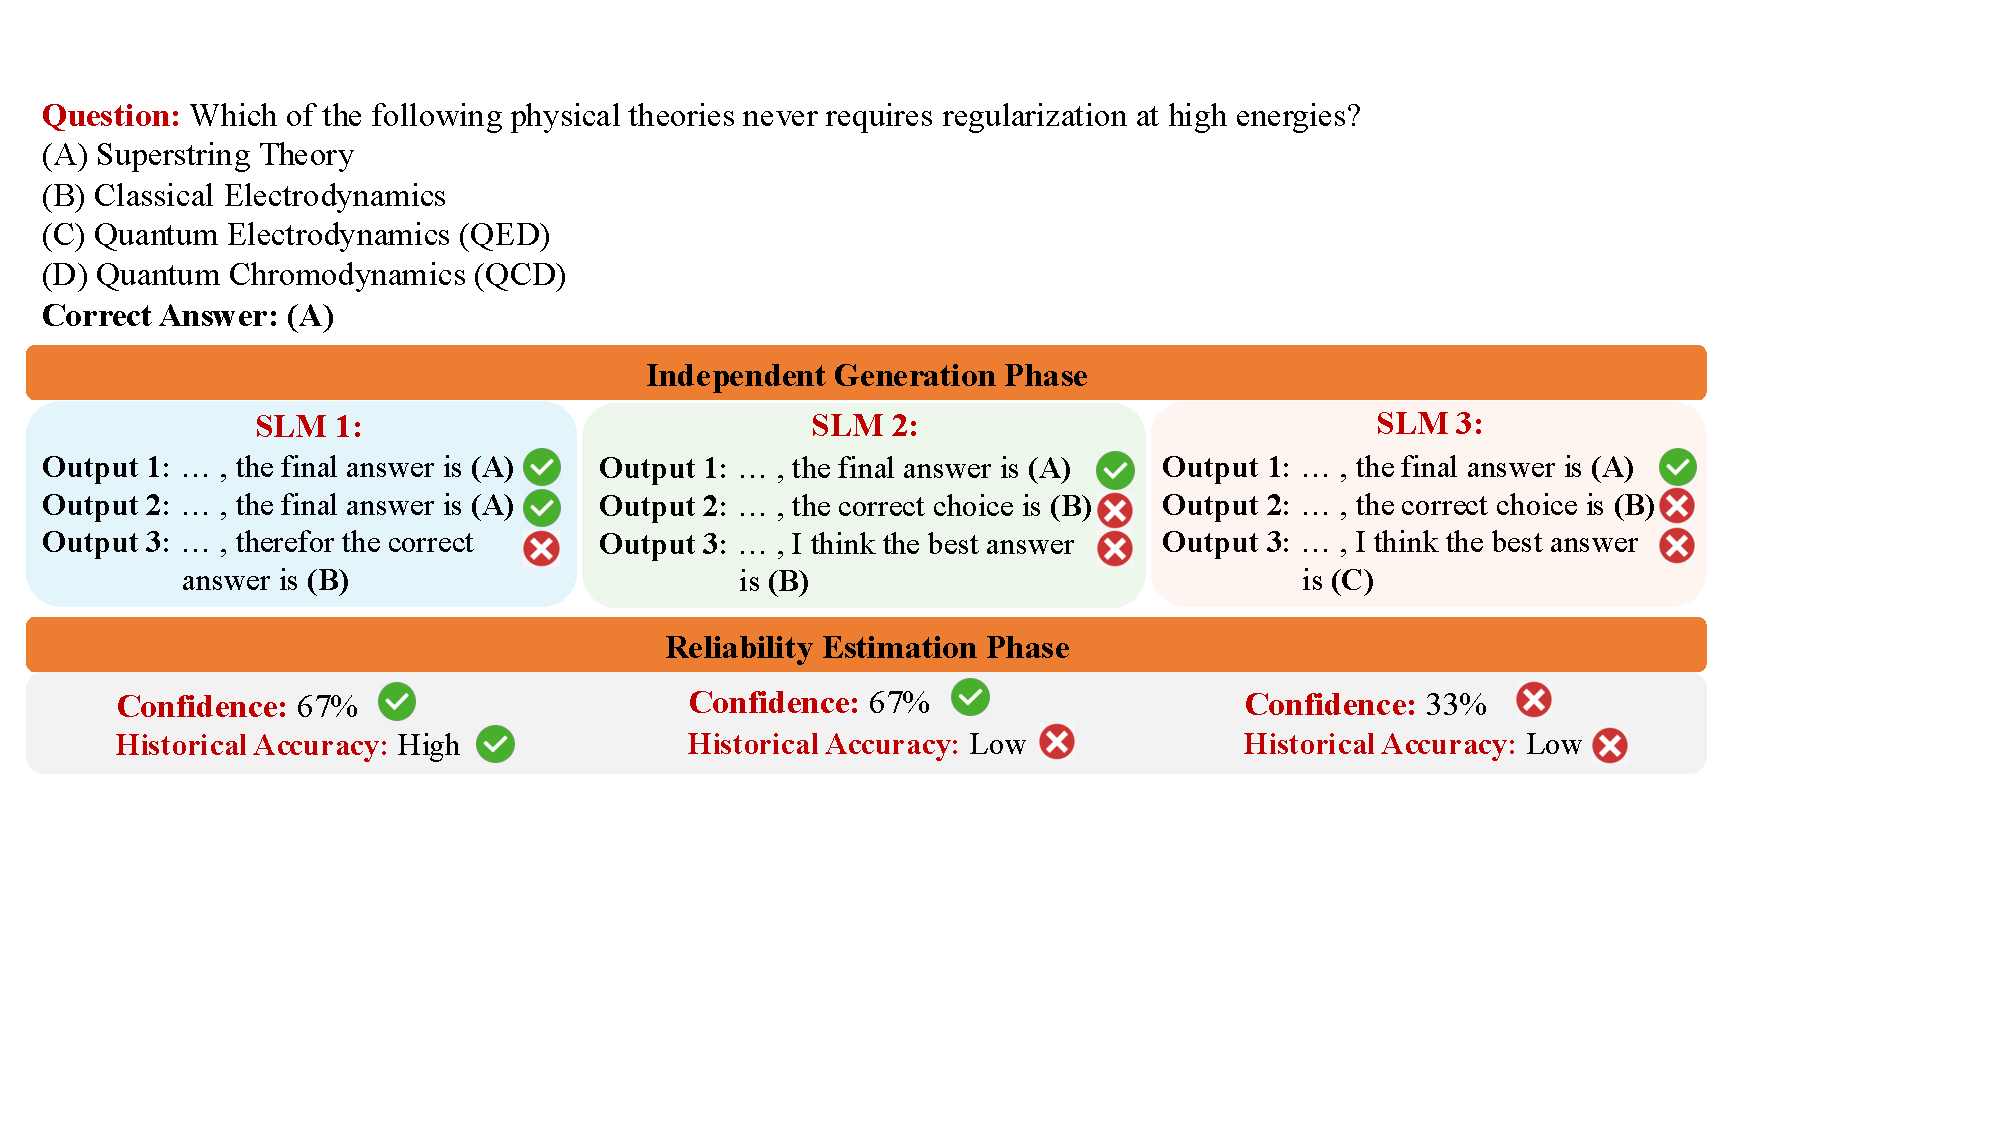
\includegraphics[width=\linewidth]{Figures/LM-Mux_workflow_v2.pdf}
  \vspace{-12pt}
  \caption{\small \textbf{Illustration of \NAME{}{} Workflow.}
(1) Each SLM first independently generates multiple outputs for the same question.
(2) The most frequent answer from each SLM is selected, and its frequency in the answer pool is used as the confidence score.
(3) The answers with the highest confidence score are selected.
(4) If multiple answers share the same confidence score, the tie is broken by selecting the answer from the SLM with the highest accuracy on the validation set. }
  \label{fig:SLM-Mux-method}
  \vspace{-20pt}
\end{figure}
% The inspiration behind our proposed approach stems from observing human problem-solving behaviors. When multiple individuals independently attempt to solve the same complex problem but are unable to communicate directly, selecting the most reliable answer becomes challenging~\cite{Condorcet1994}. Humans naturally employ metacognitive abilities, reflecting on their own responses to judge confidence~\cite{Flavell1979}. However, LLMs lack such ability and tend to exhibit overconfidence when self-assessing the accuracy of their outputs, making direct confidence querying not reliable and ineffective~\cite{geng2024surveyconfidenceestimationcalibration,yang2024trustllmsmitigateoverconfidence}. Motivated by previous works on model ensemble~\cite{gal2016dropoutbayesianapproximationrepresenting,lakshminarayanan2017simplescalablepredictiveuncertainty,wang2023selfconsistencyimproveschainthought}, we consider an alternative method: independently generating multiple samples from each model and then evaluating answer confidence based on the dispersion of these samples. By analyzing the distribution of independently generated answers and considering historical model performance metrics, we aim to reliably identify the most credible answer without explicit model self-assessment.



% By explicitly defining and enforcing aggregation protocols independent of textual interactions, we observe that \NAME{}{} method mitigates the superficial interaction issues common in traditional composition methods when applied to smaller-scale models.

\begin{figure}[t]
\begin{minipage}{\linewidth}
% \small
\begin{algorithm}[H]
\caption{\NAME{}{} Working Flow}
\label{alg:SLM-Mux}
\textbf{Input}: Models $M_1,\dots,M_n$, query $x$, samples per model $k$, validation accuracies $a_1,\dots,a_n$ \\
\textbf{Output}: Final answer $\hat{y}$
\begin{algorithmic}[1]
\Statex \textit{Independent Generation: each model produces multiple candidate answers independently}
\For{$i=1,\dots,n$}
    \State Sample $k$ answers $Y_i=\{y_i^{(1)},\dots,y_i^{(k)}\}$ from $M_i$
    \State Compute $f_i(y)=\tfrac{1}{k}\sum_{j=1}^{k}\mathbf{1}\!\left(y_i^{(j)}=y\right)$
    \State Let $y_i^*=\arg\max_{y} f_i(y)$ and set $s_i = f_i(y_i^*)$
\EndFor

\Statex \textit{Confidence Estimation: measure self-consistency and break ties by validation accuracy}
\State $S_{\max}=\max_{i} s_i$, \quad $I^*=\{\, i \mid s_i = S_{\max} \,\}$
\If{$|I^*|=1$}
    \State $i^* \gets \text{the unique index in } I^*$
\Else
    \State $i^* \gets \arg\max_{i \in I^*} a_i$
\EndIf
\State \textbf{return} $\hat{y}=y_{i^*}^*$
\end{algorithmic}
\end{algorithm}
\end{minipage}
\vspace{-5pt}
\end{figure}










% \begin{figure}[t]
%   \centering
%   \includegraphics[width=0.85\linewidth]{Figures/\NAME{}{}_workflow.pdf}
%   % \vspace{-5pt}
%   \caption{\small \textbf{Illustration of \NAME{}{} Workflow.}
% Detailed workflow of the proposed \NAME{}{} method. 
% (1) Each small language model independently generates multiple outputs from a straightforward, isolated prompt.
% (2) Responses are aggregated, and answer frequencies within each model are computed to establish a confidence score.
% (3) For tasks with finite answer spaces, responses meeting or exceeding a confidence threshold (e.g., 2/3 majority) are combined into a candidate pool.
% (4) Final selection from this pool leverages historical accuracy metrics of individual models to choose the most reliable answer.
%   }
%   \label{fig:SLM-Mux-method}
%   \vspace{-15pt}
% \end{figure}

% \vspace{-5pt}
\vspace{5pt}
\subsection{Model Selection Search for SLM-MUX Optimization}
% \vspace{3pt}
% \vspace{-3pt}
\label{sub:method-search}

% \paragraph{Intuition} In Section~\ref{sub:method-arch}, we introduced a new compositional architecture. A key question remains: which SLMs should be chosen to use in the architecture? With dozens of SLMs now available, we have access to a large model pool. Since it is not feasible to invoke every SLM in the \NAME{}{} for every given query, it is worth investigating whether there is an optimal strategy for selecting a limited subset of models for each task.
% 
% \subsubsection{Model Selection Optimization}
% \label{subsub: search}
% 
% Another motivation of model selection search is that for each task, choosing SLMs with overlapping strengths may bring little improvement, but selecting those with complementary strengths may significantly boost accuracy. For example, as shown in Figure~\ref{fig:motivation-search}, the models on the left have highly overlapping capabilities. Llama 3.2 3B offers no advantage in every subject: for most (if not all) MATH questions, if Qwen 2.5 7B cannot solve them, neither can Llama 3.2 3B. In this case, combining them provides no benefit. However, the models on the right show complementary strengths: Mistral Small 24B scores higher in some subjects, and Qwen 2.5 7B does better in others. In this case, when Qwen 2.5 7B cannot answer a question, Mistral Small 24B may succeed.
% 

At a high level, the idea of model selection search is to identify complementarity among models. The goal is not simply to add more models, but to bring new capabilities as we add models. To illustrate, Figure~\ref{fig:motivation-search} illustrates this intuition: Qwen2.5-7B consistently outperforms Llama3.2-3B across all subjects, so combining them offers no capability beyond what Qwen2.5-7B already provides. In contrast, Mistral Small 24B and Qwen2.5-7B show complementary strengths—one performs better in certain subjects while the other excels in different ones—so pairing them leads to clear gains.


We frame model selection as a search on the validation set with two competing objectives. Our search objective is formulated as follows:


% 

Our first objective is \textbf{Union Accuracy}, which reflects the overall accuracy 
of the system. The higher the union accuracy is, the more questions a system can potentially answer. Formally, let 
$\mathcal{M} = \{m_1, \ldots, m_K\}$ denote the set of candidate models and 
$\mathcal{D}$ the validation set. For each model $m_i \in \mathcal{M}$, we 
record the subset of validation instances it solves correctly. Given a candidate 
subset $S \subseteq \mathcal{M}$, the union accuracy is defined as
% \begin{equation*}
%     \text{Union Acc}(S) = \frac{1}{|\mathcal{D}|}
%     \sum_{x \in \mathcal{D}}
%     \mathbb{1}\big[\exists m \in S : m(x) \text{ is correct}\big]
% \end{equation*}
% 
\begin{equation*}
\mathrm{UnionAcc}(S) =
\frac{1}{|\mathcal{D}|}
\sum_{x \in \mathcal{D}}
\mathbf{1}\!\left\{ \exists\, m \in S \;:\; m(x)\ \text{is correct} \right\}
\end{equation*}
% 
% 
% 
% 
% 
% 
The second objective is the \textbf{Contradiction Penalty}. It captures problematic cases where overconfident wrong answers suppress correct predictions from other models. Consider two SLMs answering the same multiple-choice question three times: the first model consistently outputs ``A'' (correct), while the second consistently outputs ``B'' (incorrect but confident). Since \NAME{}{} selects based on consistency, both models would appear equally confident, making it impossible to distinguish the correct answer from the confident but wrong one. We define this penalty as the percentage of questions where at least one model consistently gives the wrong answer while another provides the correct answer:
% \begin{equation*}
% \text{Contradiction}(S) 
% = \frac{1}{|\mathcal{D}|}
% \sum_{x \in \mathcal{D}}
% \mathbb{1}\Big[
%    \exists m_1 \in S: m_1(x)\ \text{consistently wrong} \ \wedge
%    \exists m_2 \in S: m_2(x)\ \text{correct}
% \Big]
% \end{equation*}
% 
\begin{equation*}
\mathrm{Contradiction}(S) 
= \frac{1}{|\mathcal{D}|}
\sum_{x \in \mathcal{D}}
\mathbf{1}\!\Bigg\{
   \begin{array}{l}
   \exists\, m_1 \in S:\ m_1(x)\ \text{consistently wrong}, \\[4pt]
   \exists\, m_2 \in S:\ m_2(x)\ \text{correct}
   \end{array}
\Bigg\}
\end{equation*}
% 
% 
% 
% 
% 
% 
% 
% 
The final objective balances these competing factors:
% 
\begin{equation*}
\mathcal{O}(S) \;=\; Acc(S) \;-\; \lambda \cdot Contradiction(S),
\end{equation*}
% 
% 
% 
Where $\lambda$ is a hyperparameter. Since the number of candidate models is not very large, 
we perform an exhaustive search. We present visualization of the two search objectives and evaluation of the searched model selection in Section~\ref{sub:search-results}.

% \vspace{-5pt}
\subsection{Compute Scaling Strategies}
% \vspace{-3pt}
\label{sec:scaling}
% Building on the \NAME{}{} and model selection search, we next scale test-time compute to further improve the accuracy. We explore two dimensions for scaling compute at test time. These dimensions are described as follows:

% (1) Scaling Model Counts: As we scale the model counts used in the composition by adding more SLMs with complementary strengths, we expect the overall accuracy to improve. For each budgeted number of models, we use the search method proposed in Section~\ref{sub:method-search} to identify the best selection from the pool. 

% (2) Scaling Samples per Model: For a fixed model selection, we can increase the compute budget by scaling the number of samples drawn by each model. Since confidence is evaluated by counting the frequency of majority answers, adding more samples per model is expected to provide a more accurate confidence estimate.
\begin{wrapfigure}{r}{0.6\textwidth} 
\vspace{-20pt}
    \centering
    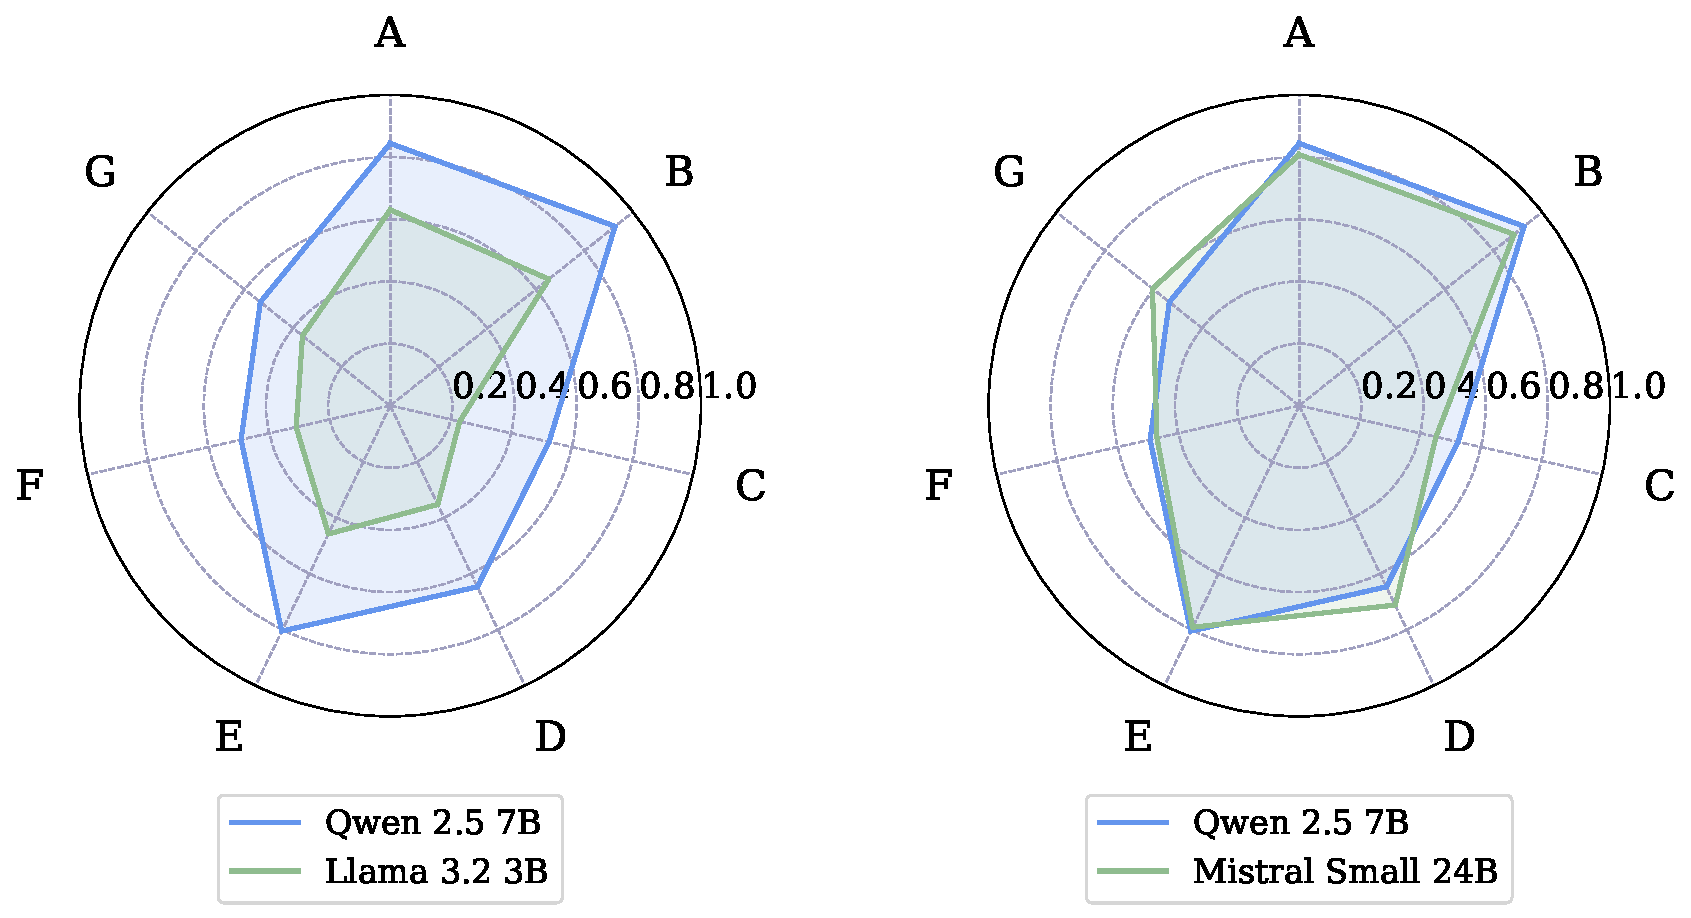
\includegraphics[width=\linewidth]{Figures/radar_compare_pairs.pdf}
    \vspace{-20pt}
    \caption{\textbf{Comparison of Model Choices}. Accuracy on 7 subjects for two model selection settings on MATH dataset. Subjects are denoted as: A = Prealgebra, B = Algebra, C = Intermediate Algebra, D = Number Theory, E = Counting \& Probability, F = Geometry, G = Precalculus.}

    \vspace{-10pt}
    \label{fig:motivation-search}
\end{wrapfigure}
% After we select the model, the next question is how much test-time compute budget should we use to wisely improve accuracy. We next scale test-time compute to further improve the accuracy. We empirically explore two dimensions for scaling compute at test time to find the best accuracy. These dimensions are described as follows:


% At a high level, given that scaling compute at test-time is a proven strategy for improving accuracy, we also explore this direction.
Next, we empirically investigate two dimensions of test-time scaling to further enhance the performance of our \NAME{}{} with selected models.

\looseness=-1
\textbf{Adding More Participating Model Types:} As we scale the model participating model types used in the system by adding more SLMs with complementary strengths, we expect the overall accuracy to improve. For each budgeted number of models, we use the search method proposed in Section~\ref{sub:method-search} to identify the best selection from the pool. 

\textbf{Drawing More Samples per Model:} For a fixed model selection, we can increase the compute budget by scaling the number of samples drawn by each model. Since confidence is evaluated by counting the frequency of majority answers, adding more samples per model is expected to provide a more accurate confidence estimate.


These two compute scaling dimensions are evaluated in Section~\ref{sub:scaling-results}.

% \label{subsub:tuning}
%  The architecture described above provides an identical prompt to each model. This "one-size-fits-all" approach is inherently limited, as it fails to account for the fact that different models have distinct strengths, weaknesses, and reasoning patterns. Therefore, prompts should be tailored to each model to leverage its specific advantages and mitigate its shortcomings.

% Instead of tuning the prompts for the entire compositional system in an end-to-end manner, we adopted an approach from prior work. We tuned the prompt for each model individually. These optimized prompts were then integrated into our \NAME{}{} framework, where each model was assigned its own tailored prompt in place of the original, uniform one.

% Specifically, we employed a genetic algorithm-inspired approach to tune the prompts. The process begins with the original uniform prompt as the initial seed. For each model, we sample an evaluation set of 25 questions from the dataset. We then iterate the following process ten times:

% First, we assess the performance of the current prompt with its corresponding model on the evaluation set. Based on the results, we generate new candidate prompts using a separate "Tuner LLM" which applies one of two strategies:

% \begin{enumerate}
%     \item \textbf{Mutation}: The Tuner LLM is provided with the current prompt, along with one correctly and one incorrectly answered question from the evaluation set, and is instructed to revise the prompt.
%     \item \textbf{Generation}: The Tuner LLM is provided only with the correct and incorrect examples and is tasked with generating an entirely new prompt from scratch.
% \end{enumerate}

% We observed that the optimal strategy (Mutation vs. Generation) is sensitive to the specific model and dataset being used. As a further detail, the models whose prompts were being tuned consistently used a sampling temperature of 0. We also experimented with using a non-zero temperature, which is a necessary condition for the multi-sample strategy in our \NAME{}{} method. However, we found that tuning prompts with multiple samples led to inconsistent impacts on final performance. Therefore, for simplicity and reproducibility, we opted to set the temperature to 0 during the prompt tuning phase.


% A key advantage of this method is that optimization occurs entirely at inference time. This avoids computationally expensive procedures like fine-tuning or retraining, which require modifying the model's weights.




% \input{Sections/pbc}
% % \subsection{Combining  }

% \textbf{Majority voting only improves accuracy for simpler tasks.} Our experimental results indicate that majority voting enhances accuracy solely when applied to simple questions, and it does not outperform the best individual LLM prediction for complex problems. Through detailed analysis, we observed that for simpler questions, disagreements among individual LLM predictions are typically limited, whereas for complex problems, such disagreements become significantly pronounced. We model this problem by assuming each LLM independently generates answers, where each answer has a probability \( p \) of being correct. Under this assumption, the theoretical accuracy \( A(N, p) \) achievable by majority voting among \( N \) independently predicting models is described by the cumulative probability of a binomial distribution:

% \begin{equation}
% A(N, p) = \Pr\left(X \ge \left\lceil \frac{N}{2} \right\rceil\right) = \sum_{k=\lceil \frac{N}{2} \rceil}^{N} \binom{N}{k} p^{k}(1 - p)^{N - k}, \quad X \sim \text{Binomial}(N, p)
% \end{equation}

% In Figure~\ref{fig:composed_accuracy}, we plot the theoretical accuracy \( A(N, p) \) as a function of individual accuracy \( p \) for different numbers of models (\( N = 3, 5, 7, 9 \)). This plot clearly demonstrates that composed accuracy \( A(N, p) \) surpasses individual accuracy \( p \) only when \( p > 0.5 \). Conversely, for values of \( p \leq 0.5 \), majority voting negatively impacts performance, indicating that aggregation is counterproductive when individual models perform near or below chance.


% \begin{figure}[h]
% \centering
% 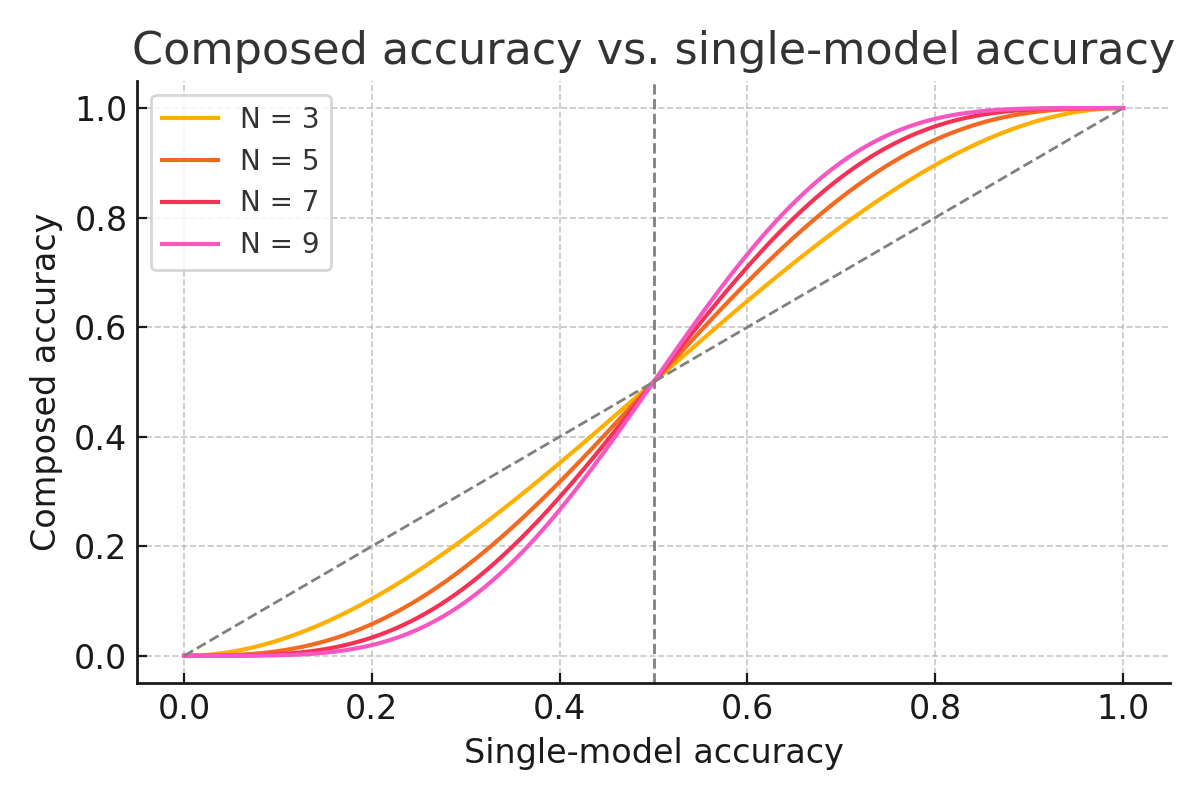
\includegraphics[width=0.7\textwidth]{Figures/majority_accuracy.png}
% \caption{Theoretical analysis of composed accuracy vs. single-model accuracy for different numbers of models $N$.}
% \label{fig:composed_accuracy}
% \end{figure}

% Inspired by this

% Algorithm~\ref{alg:adaptive-routing} formally outlines this adaptive routing procedure:

% \begin{algorithm}[h]
% \caption{Adaptive Routing for Compositional LLMs}
% \label{alg:adaptive-routing}
% \textbf{Input}: Models \( M_1,\dots,M_n \), query \( x \), complex compositional method \( C \), threshold \( 0.5 \) \\
% \textbf{Output}: Final answer \( \hat{y} \)
% \begin{algorithmic}[1]
% \For{\( i=1,\dots,n \)}
%     \State \( y_i \leftarrow M_i(x) \) \Comment{initial independent predictions}
% \EndFor
% \State Compute \( n^* = \max_{y}\sum_{i=1}^{n}\mathbf{1}(y_i = y) \) \Comment{number of majority votes}
% \State Set hyperparameter \(\alpha=1\) for uniform smoothing
% \State Estimate correctness probability \( \hat{p} = \frac{n^*+\alpha}{n+2\alpha} \) via Beta posterior
% \If{\( \hat{p} > 0.5 \)}
%     \State \( \hat{y} \leftarrow \) majority vote over predictions \( y_i \) \Comment{simple aggregation}
% \Else
%     \State \( \hat{y} \leftarrow C(M_1,\dots,M_n, x) \) \Comment{advanced compositional method}
% \EndIf
% \State \textbf{return} \( \hat{y} \)
% \end{algorithmic}
% \end{algorithm}








\vspace{3pt}
\section{Experiments}
\vspace{3pt}
% \vspace{-3pt}
\label{sect:experiment}


In our experiments, we first demonstrate the fundamental limitations of existing discussion-based orchestration methods when applied to SLMs (Section~\ref{sec:comparison}). We then evaluate the proposed \NAME{} in Section~\ref{sub:vanilla}. In Section~\ref{sub:search-results}, we access our proposed search strategy. Finally, in Section~\ref{sub:scaling-results}, we examine the compute scaling strategies.
% We design a comprehensive experimental setup across multiple datasets and model scales to rigorously assess these questions.

\vspace{3pt}
\subsection{Existing Discussion-Based Orchestration Methods Harm SLM Performance}
\vspace{3pt}
\label{sec:comparison}

% We evaluate three discussion-based composition architectures: LLM-Debate~\citep{du2023improvingfactualityreasoninglanguage}, Mixture-of-Agents~\citep{wang2024mixtureofagentsenhanceslargelanguage}, and Multi-Agent Verification~\citep{lifshitz2025multiagentverificationscalingtesttime}. We use the same experimental settings for SLMs and frontier LLMs; we vary only the choice of models between a small-sized group and a frontier (often larger) group.

To understand whether orchestration methods developed for frontier LLMs are suitable for SLMs, we conduct a systematic comparison across model scales. We evaluate three prominent discussion-based methods—LLM-Debate~\citep{du2023improvingfactualityreasoninglanguage}, Mixture-of-Agents~\citep{wang2024mixtureofagentsenhanceslargelanguage}, and Multi-Agent Verification~\citep{lifshitz2025multiagentverificationscalingtesttime} —using identical experimental settings on both SLMs (Llama 3.1 8B~\citep{jiang2024mixtralexperts}, Mistral 8×7B~\citep{grattafiori2024llama3herdmodels}, Gemma 2 27B) and frontier LLMs (DeepSeek V3~\citep{deepseekai2025deepseekv3technicalreport}, Gemini 2.0 Flash~\citep{google2025gemini2flash}, GPT-4o~\citep{openai2024gpt4ocard}). Evaluation is conducted on MATH and GPQA datasets using original implementations and prompts.


\paragraph{Results} As shown in Figure~\ref{fig:small-large-accuracy}, discussion-based methods generally outperform the single best-performing models in the frontier LLM group, achieving up to a 2\% increase in accuracy. However, when applied to SLMs, these discussion-based methods fail to outperform the best single model in the orchestration, and even incur accuracy drops of up to 5.5\%. This performance gap is observed across all three methods and both benchmarks. 

To understand this counterintuitive result, we analyze SLM behavior in discussion settings. We find that discussion-based methods amplify rather than correct errors in SLMs due to a key limitations: SLMs tend to exhibit groupthink, reinforcing incorrect reasoning during discussions rather than correcting mistakes. Additional analysis and demonstration is provided in the Appendix~\ref{sec:slm-failure}.



\begin{figure}[htbp]
  \centering
  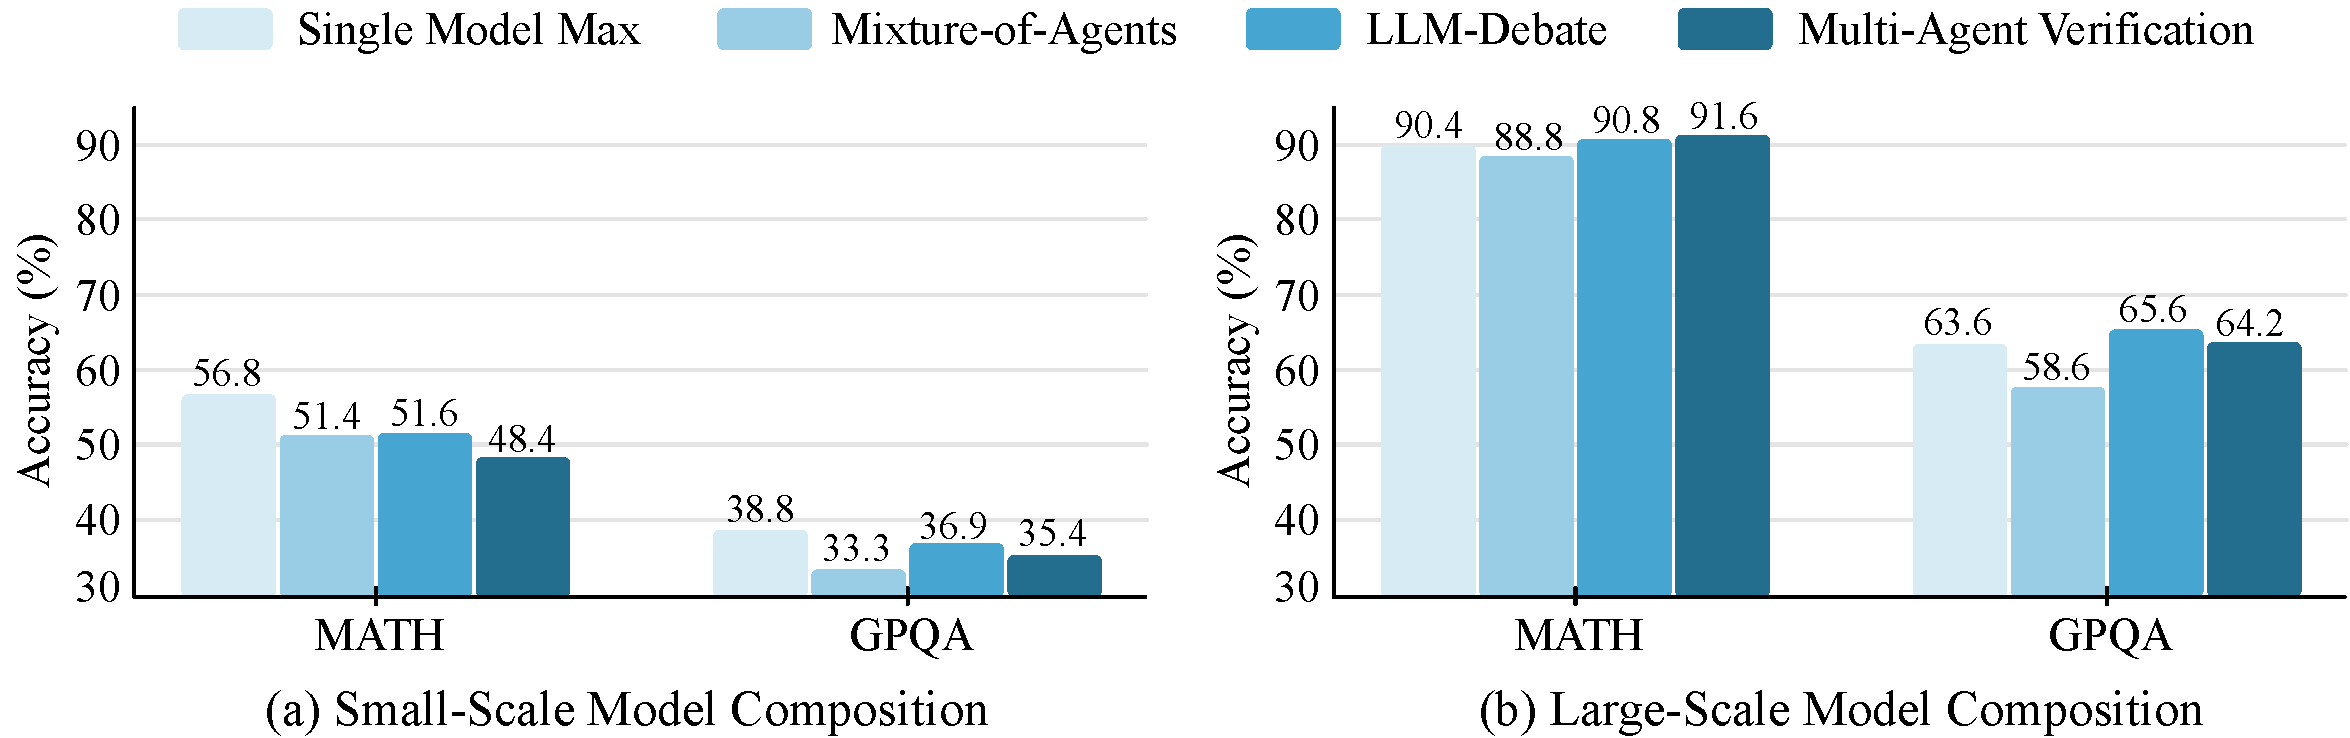
\includegraphics[width=0.9\linewidth]{Figures/Small-large-acc-light-blue_v2.pdf}
  \vspace{-8pt}
  \caption{\small \textbf{Comparison of discussion-based orchestration when invoking SLMs and LLMs.} We compare three orchestration methods (Mixture-of-Agents, LLM-Debate, and Verification) using (a) SLMs (Llama 3.1 8B, Mistral 8$\times$7B, Gemma 2 27B) and (b) frontier LLMs (DeepSeek V3, Gemini 2.0 Flash, GPT-4o) on the \textsc{MATH} and \textsc{GPQA} datasets. The baseline (\textit{Single-Model Max}) reflects the best performance of individual models. A orchestration is considered successful if it surpasses Single-Model Max.}\label{fig:small-large-accuracy}
  \vspace{-10pt}
\end{figure}



\vspace{3pt}
\subsection{\NAME{} Achieves SLM Orchestration Where Existing Methods Fail}
\vspace{3pt}
\label{sub:vanilla}

\begin{wrapfigure}{r}{0.4\textwidth}
    \centering
    \vspace{-20pt}
    \includegraphics[width=.85\linewidth]{Figures/math_distribution_pie.pdf}
    \caption{\textbf{Final Output Attribution}. We report the percentage of outputs contributed by each model on the MATH dataset for our \NAME{}. These results are from the same run as in Table~\ref{tab:composition-combined}.}
    \label{fig:output_percentage_math}
    \vspace{-5pt}
\end{wrapfigure}

To evaluate whether our proposed \NAME{} can successfully orchestrate SLMs, we test it against the same baselines from Section~\ref{sec:comparison}.  We use Mistral 8$\times$7B, LLaMA 3.1 8B, and Gemma 2 27B~\citep{gemmateam2024gemma2improvingopen} as base models. We implement the \NAME{} as follows. First, we generate three rounds of answers with a temperature of 0.3. Next, we compute a confidence score by counting how often the most common answer appears across these rounds. The final answer for each model is chosen as the most frequent one; in the case of a tie, we select the answer from the model with the highest validation accuracy. We evaluate three types of baselines. First, we measure the accuracies of individual models and report the best-performing ones. Next, for comparison with existing discussion-based methods, we include LLM-Debate~\citep{du2023improvingfactualityreasoninglanguage}, Mixture-of-Agents~\citep{wang2024mixtureofagentsenhanceslargelanguage}, and Multi-Agent Verification~\citep{lifshitz2025multiagentverificationscalingtesttime}. We follow the original workflow designs and prompts described in their papers. Experiments are conducted on three benchmark datasets: MATH~\citep{hendrycks2021measuringmathematicalproblemsolving}, GPQA~\citep{rein2023gpqagraduatelevelgoogleproofqa}, and GSM8K~\citep{cobbe2021trainingverifierssolvemath}. 




% \begin{figure}[hbtp]
%     \centering
%     \includegraphics[width=\textwidth]{iclr2026/Figures/math_distribution_pie.pdf}
%     \vspace{-20pt}
%     \caption{\textbf{Final Output Attribution}. We report the percentage of outputs contributed by each model on the MATH dataset for our \NAME{}. These results are from the same run as in Table~\ref{tab:composition-combined}. }
%     \vspace{-10pt}
%     \label{fig:output_percentage_math}
% \end{figure}


\looseness=-1
\paragraph{Results} Table~\ref{tab:composition-combined} summarizes the results. In our experiments, we find that for SLMs, existing orchestration methods do not consistently outperform the strongest individual base models or self-consistency approaches. In contrast, our \NAME{} generally achieves an accuracy gain. Compared with other approaches, our method yields up to a 13.4\% improvement on MATH, up to 8.8\% on GPQA, and up to 7.0\% on GSM8K.  These results demonstrate that the \NAME{} itself provides a clear advantage over alternative orchestration approaches at the architectural level. 

To better illustrate our proposed \NAME{}, we plot the output attribution for the MATH experiment (Table~\ref{tab:composition-combined}) in Figure~\ref{fig:output_percentage_math}. By selecting diverse outputs from the generation, \NAME{} leverages the complementary strengths of different SLMs.




% % -------- Table 2: Composition Results --------
% \begin{table}[t]
% \centering
% \small
% \begin{tabular}{lccc}
% \toprule
% \textbf{Method} & \textbf{MATH Acc (\%)} & \textbf{GPQA Acc (\%)} & \textbf{GSM8K Acc (\%)} \\
% \midrule
% Mixture-of-Agents          & 51.4 & 33.3 & 81.6 \\
% LLM-Debate                  & 51.6 & 36.8 & 80.8 \\
% Multi-Agent Verification    & 48.4 & 35.3 & 86.4 \\
% \textbf{\NAME{} (Ours)}         & \textbf{$63.0 \pm 2.16$} & \textbf{$41.9 \pm 3.52$ } & \textbf{$88.4 \pm 1.43$} \\
% \midrule
% Single-Best                 & 56.8 & 38.9 & 84.2 \\
% Single-Best-SC                 & $58.0 \pm 2.21$ & $42.4 \pm 3.53$ & $86.8 \pm 1.51$ \\
% Upper Bound                 & 64.6 & 57.0 & 92.0 \\
% \bottomrule
% \end{tabular}
% \vspace{-5pt}
% \caption{\small \textbf{\NAME{} Improves Reasoning Performance.} Accuracy of orchestration methods on MATH, GPQA, and GSM8K.}
% \label{tab:composition-combined}
% \vspace{-5pt}
% \end{table}

\begin{table}[ht]
\centering
\setlength{\tabcolsep}{15pt}
\renewcommand{\arraystretch}{0.9}
\resizebox{\textwidth}{!}{
\small
\vspace{-5pt}
\begin{tabular}{lccc}
\toprule
\textbf{Method} & \textbf{MATH Acc (\%)} & \textbf{GPQA Acc (\%)} & \textbf{GSM8K Acc (\%)} \\
\midrule
Mixture-of-Agents          & 51.4 $\pm$ 2.2 & 33.3 $\pm$ 3.4 & 81.6 $\pm$ 1.7 \\
LLM-Debate                 & 51.6 $\pm$ 2.2 & 36.8 $\pm$ 3.4 & 80.8 $\pm$ 1.8 \\
Multi-Agent Verification   & 48.4 $\pm$ 2.2 & 35.3 $\pm$ 3.4 & 86.4 $\pm$ 1.5 \\
\textbf{\NAME{} (Ours)}    & \textbf{61.8 $\pm$ 1.2} & 42.1 $\pm$ 0.3 & \textbf{87.8 $\pm$ 0.6} \\
\midrule
Single-Best                & 56.8 $\pm$ 2.2 & 38.9 $\pm$ 3.5 & 84.2 $\pm$ 1.6 \\
Single-Best-SC             & 58.0 $\pm$ 2.2 & \textbf{42.4 $\pm$ 3.5} & 86.8 $\pm$ 1.5 \\
% Upper Bound                & 64.6 $\pm$ 2.14 & 57.0 $\pm$ 3.54 & 92.0 $\pm$ 1.21 \\
\bottomrule
\end{tabular}
}
\vspace{-5pt}
\caption{\small \textbf{Accuracy with Standard Error.} The standard error across MATH, GPQA, and GSM8K for various methods. }
\label{tab:composition-combined}
\vspace{-5pt}
\end{table}




% Please ensure you have these two packages in your preamble (after \documentclass{...})
% \usepackage{tabularx}
% \usepackage{array}

% \begin{table}[t]
% \centering
% \small
% % Corrected a typo in the caption (founded -> found)
% \caption{\small \textbf{Model Combination Search results} Best model combinations found for different datasets and objectives across varying numbers of models involved (K). For clarity we just show K = 1, 2, 3 here, full results with K up to 7 can be found in appendix. }
% \label{tab:SLM-Mux-model-search-heterogeneity-adjusted}
% % Use the tabularx environment with a total width of \textwidth
% % Keep 'll' columns as is, use left-aligned, auto-adjusting X columns for the last three
% \begin{tabularx}{\textwidth}{ll >{\raggedright\arraybackslash}X >{\raggedright\arraybackslash}X >{\raggedright\arraybackslash}X}
% \toprule
% \textbf{Dataset} & \textbf{Objective} & \textbf{K=1} & \textbf{K=2} & \textbf{K=3} \\
% \midrule
% \multirow{4}{*}{\textbf{MATH}}
%  & Accuracy
%  & Qwen2.5-7B  % Abbreviated "Instruct"
%  & Mistral Small 24B  \newline Qwen2.5-7B 
%  & Gemma 2 27B \newline Mistral Small 24B  \newline Qwen2.5-7B  \\
% \cmidrule{2-5}
%  & Heterogeneity
%  & --
%  & Gemma 2 27B \newline Llama 3.1 8B 
%  & Gemma 2 27B \newline Llama 3.1 8B \newline Mixtral 8x7B Instruct  \\
% \midrule
% % ==== GPQA ====
% \multirow{2}{*}{\textbf{GPQA}}
%  & Accuracy
%  & Gemma 2 27B
%  & Gemma 2 27B \newline Mistral Small 24B
%  & Gemma 2 27B \newline Mistral Small 24B \newline Mixtral 8x7B Instruct \\
%  \cmidrule{2-5}
%  & Heterogeneity
%  & --
%  & Gemma 2 27B \newline Mistral Small 24B
%  & Llama 3.1 8B \newline Mixtral 8x7B Instruct \newline Qwen2.5-7B \\
% \midrule

% % ==== GSM8K ====
% \multirow{2}{*}{\textbf{GSM8K}}
%  & Accuracy
%  & Qwen2.5-7B
%  & Mistral Small 24B \newline Qwen2.5-7B
%  & Llama 3.1 8B \newline Mistral Small 24B \newline Qwen2.5-7B \\
%  \cmidrule{2-5}
%  & Heterogeneity
%  & --
%  & Gemma 2 27B \newline Llama 3.1 8B
%  & Gemma 2 27B \newline Llama 3.1 8B \newline Mixtral 8x7B Instruct \\
% \midrule

% % ==== MMLU ====
% \multirow{2}{*}{\textbf{MMLU}}
%  & Accuracy
%  & Mistral Small 24B
%  & Mistral Small 24B \newline Qwen2.5-7B
%  & Gemma 2 27B \newline Mistral Small 24B \newline Qwen2.5-7B \\
%  \cmidrule{2-5}
%  & Heterogeneity
%  & --
%  & Llama 3.1 8B \newline Mixtral 8x7B Instruct
%  & Llama 3.1 8B \newline Mixtral 8x7B Instruct \newline Qwen2.5-7B \\
% \bottomrule
% \end{tabularx}
% \end{table}

% \begin{table*}[t!]
% \centering
% \begin{tabular}{l@{\hspace{3em}}ccc@{\hspace{3em}}ccc}
% \toprule
% \multirow{2}{*}{\textbf{Benchmark}} & \multicolumn{3}{c}{\textbf{Group 1}} & \multicolumn{3}{c}{\textbf{Group 2}} \\
% \cmidrule(lr){2-4} \cmidrule(lr){5-7}
% & \begin{tabular}[c]{@{}c@{}}Best Single\\ (Acc. \%)\end{tabular} & \begin{tabular}[c]{@{}c@{}}Composed\\ (Acc. \%)\end{tabular} & \begin{tabular}[c]{@{}c@{}}$\Delta$\\ (Gain)\end{tabular} & \begin{tabular}[c]{@{}c@{}}Best Single\\ (Acc. \%)\end{tabular} & \begin{tabular}[c]{@{}c@{}}Composed\\ (Acc. \%)\end{tabular} & \begin{tabular}[c]{@{}c@{}}$\Delta$\\ (Gain)\end{tabular} \\
% \midrule
% MATH & $75.5 \pm 1.5$ & $80.0 \pm 0.7$ & $+4.5$ & $75.5 \pm 1.5$ & $77.7 \pm 0.7$ & $+2.2$ \\
% GPQA & $45.1  \pm  2.8$ & $49.5  \pm  1.8$ & $+4.4$ & $45.1  \pm  2.8$ & $48.8  \pm  0.8$ & $+3.6$ \\
% GSM8K & $88.5 \pm 0.7$ & $92.8 \pm 0.6$ & $+4.3$ & $80.8 \pm 2.1$ & 
% $85.2 \pm 0.7$& $+4.4$ \\
% % MMLU & $77.2 \pm 0.8$ &  $74.5 \pm 0.8$ & $-2.7$ & $77.2 \pm 0.8$ & $73.4 \pm 0.7$ & $-3.8$ \\
% \bottomrule

% \end{tabular}
% \vspace{-10pt}
% \caption{Evaluation results of the search  }
% \label{tab:final_results}
% \vspace{-10pt}
% \end{table*}




% \begin{table*}[t!]
% \centering
% \caption{Performance improvement from applying our Heterogeneity-Aware Instruction Training (HAIT).}
% \label{tab:hait_ablation}
% \begin{tabular}{l@{\hspace{3em}}ccc}
% \toprule
% \multirow{2}{*}{\textbf{Benchmark}} & \multicolumn{3}{c}{\textbf{Ensemble (Max Accuracy Objective)}} \\
% \cmidrule(lr){2-4}
% & \begin{tabular}[c]{@{}c@{}}Base Ensemble\\ (Acc. \%)\end{tabular} & \begin{tabular}[c]{@{}c@{}}+ HAIT\\ (Acc. \%)\end{tabular} & \begin{tabular}[c]{@{}c@{}}$\Delta$\\ (Gain)\end{tabular} \\
% \midrule
% MATH & 77.7 & \textbf{78.0} & +0.2 \\
% GPQA & xx.x & \textbf{xx.x} & +x.x \\
% GSM8K & xx.x & \textbf{xx.x} & +x.x \\
% MMLU & xx.x & \textbf{xx.x} & +x.x \\
% \bottomrule
% \end{tabular}
% \end{table*}






\vspace{3pt}
\subsection{Model Selection Search Boosts \NAME{} Performance}
\vspace{3pt}
\label{sub:search-results}
% \vspace{-3pt}

% To evaluate our proposed model selection search, we first construct a validation set by sampling 500 questions from the training splits of MATH, MMLU, GPQA, and GSM8K. This set is kept distinct from the final test data to prevent contamination.

% Our pool of candidate models includes Gemma 2 27B, Llama 3.1 8B, Mistral Small 24B~\citep{mistral_small_24b_instruct}, Mixtral 8x7B, and Qwen2.5 7B~\citep{qwen2025qwen25technicalreport}. To gather performance data for our search, we generate three independent responses for each question from each model using a temperature of 0.5. This data collection process is repeated three times to ensure stable accuracy measurements.

% Using this collected data, we search for optimal model orchestrations by varying the number of models ($K$) from 2 to 5. The search is guided by the objective function defined in Section~\ref{sect:method}, which balances union accuracy and a contradiction penalty with a fixed hyperparameter $\lambda=1$. The behavior of this objective across different values of $K$ is visualized in Figure~\ref{fig:search_objectives}.

% For our primary analysis, we focus on the simplest yet practical case of finding the best two-model orchestrations ($K=2$). Table~\ref{tab:SLM-Mux-model-search-candidates-ruled} presents the top-performing pairs, from which we select two (Group 1 and Group 2) for a final, rigorous evaluation. To obtain robust results, we run these selected orchestrations three times on the test set and report their mean performance and variance in Table~\ref{tab:final_results}.




\begin{figure}[hbtp]
    \centering
    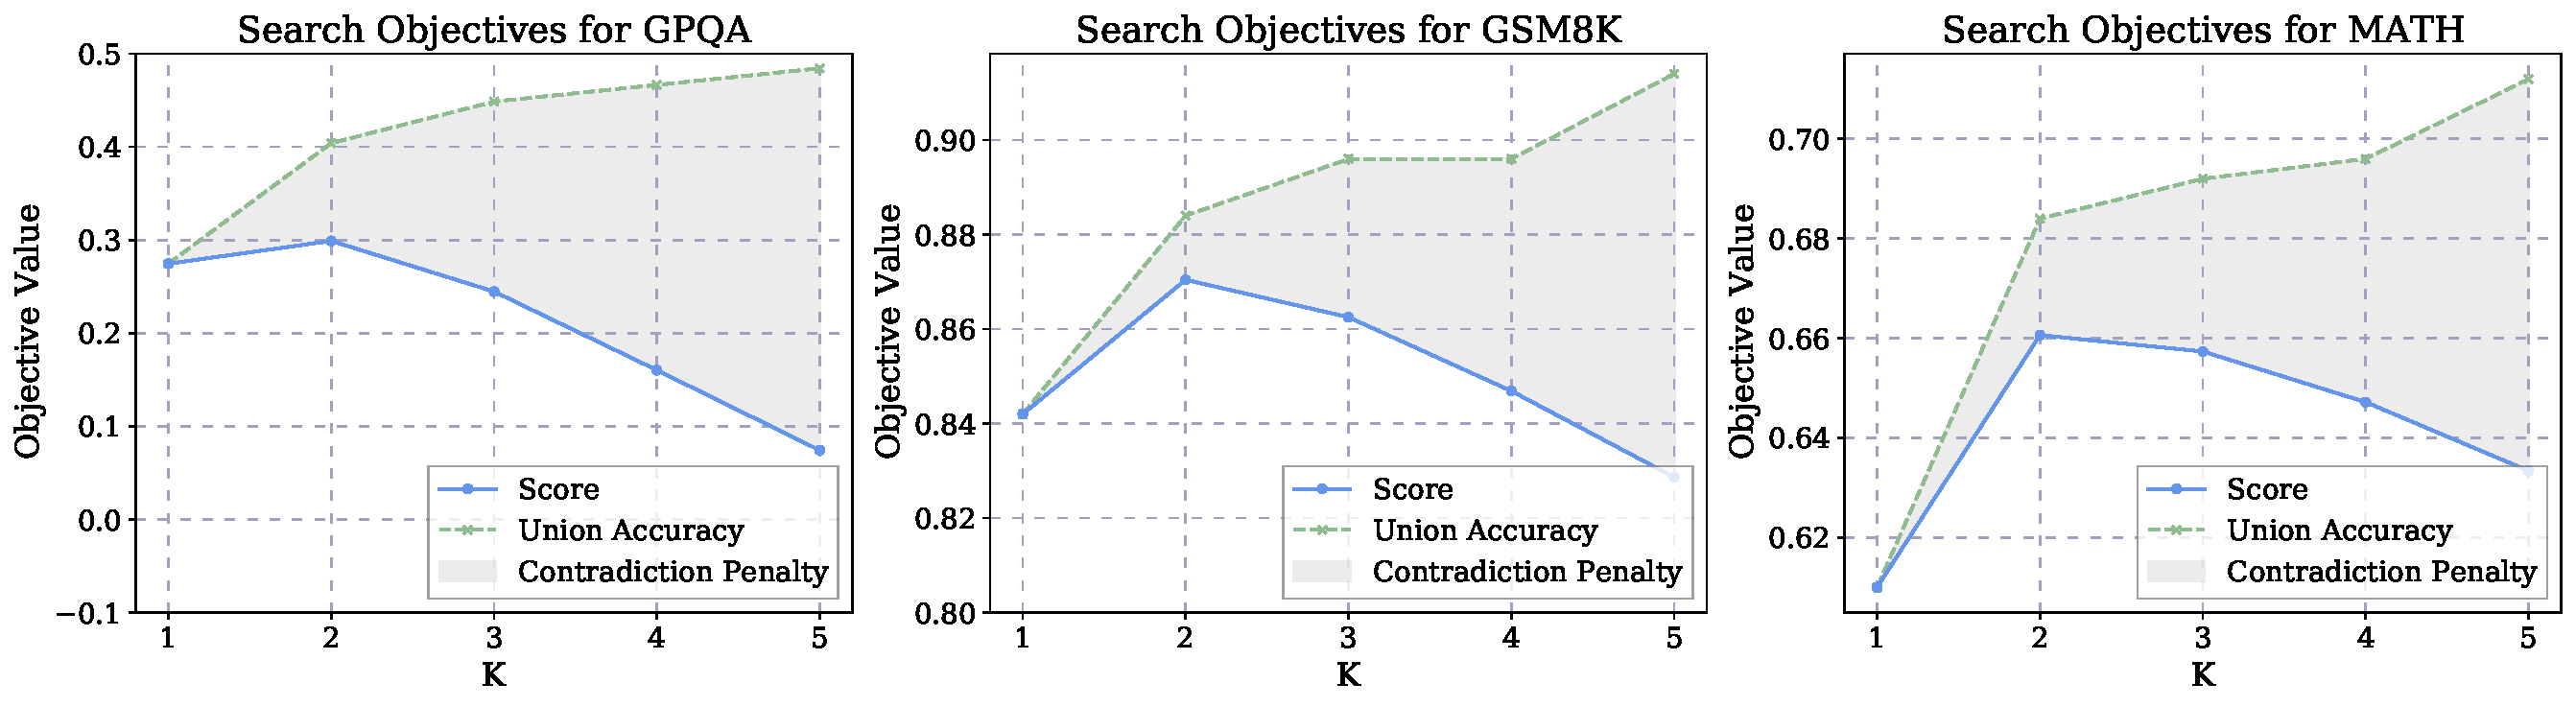
\includegraphics[width=\textwidth]{Figures/search_summary_comparison.pdf}
    \vspace{-20pt}
    \caption{\textbf{Union Accuracy and Contradiction Penalty both Increases as more models are added}. We plot the search objectives as the number of models (K) increases from 2 to 5 across three benchmarks. The green line denotes the union accuracy across models, the grey area indicates the contradiction penalty, and the blue line represents the overall search objective score. }
    % \vspace{-5pt}
    \label{fig:search_objectives}
\end{figure}


% \paragraph{Discussion \& Takeaways}
% Our results highlight two key takeaways. 
% First, model selection search is crucial for unlocking the potential of the \NAME{}. As shown in Table~\ref{tab:composition-combined}, naively combining three models without search provides little improvement over the single best model on the GPQA benchmark. In sharp contrast, our search-based method identifies a two-model orchestration that boosts accuracy by 4.4\% (Table~\ref{tab:final_results}), demonstrating the clear value of our approach.

% Second, the search process addresses a trade-off. Figure~\ref{fig:search_objectives} illustrates that as the number of models ($K$) in a orchestration increases, the union accuracy also increases. However, this is counterbalanced by a rise in the contradiction penalty, which indicates a higher frequency of conflicting predictions. This suggests that an effective model orchestration is determined by achieving a favorable balance between the union accuracy and contradiction.

\looseness=-1
To examine whether model selection search benefits \NAME{}, we construct a validation set of 500 questions sampled from the training splits of MATH, GPQA, and GSM8K. The candidate pool consists of five SLMs: Gemma 2 27B, Llama 3.1 8B, Mistral Small 24B~\citep{mistral_small_24b_instruct}, Mixtral 8$\times$7B, and Qwen2.5 7B~\citep{qwen2025qwen25technicalreport}. For each question, we collect three independent generations per model with temperature 0.5, repeating this process three times to obtain stable accuracy estimates.
The search procedure considers orchestrations with $K=2$ to $5$ models and is guided by an objective function mentioned in Section~\ref{sect:method}, with hyperparameter $\lambda=1$. The behavior of this objective is illustrated in Figure~\ref{fig:search_objectives}, showing the trade-off as $K$ increases. For simplicity, we select two representative two-model combinations from the search results for evaluation on the test set.

\paragraph{Results} Table~\ref{tab:composition_results_combined} summarizes the outcome of the search. The table lists the top-performing two-model combinations identified on the validation set, along with their evaluation on the held-out test set. Across benchmarks, these optimized orchestrations yield consistent improvements over the strongest individual models: accuracy increases by 4.5\% on MATH, 4.4\% on GPQA, and 4.3\% on GSM8K. This contrasts with Section~\ref{sub:vanilla}, where naive three-model combinations provide little to no benefit on GPQA. Figure~\ref{fig:search_objectives} further illustrates the underlying trade-off: while union accuracy rises with additional models, the contradiction penalty also grows, emphasizing that effective orchestration requires balancing these competing factors rather than simply enlarging the orchestration size.



% \begin{table}[hbtp]
% \centering
% \small


% \begin{tabular}{lll}
% \toprule
% \textbf{Dataset} & \textbf{Group 1} & \textbf{Group 2} \\
% \midrule
% \textbf{MATH}    & \makecell[l]{Mistral Small 24B \\ Qwen2.5 7B}         & \makecell[l]{ Qwen2.5 7B \\ Llama 3.1 8B} \\
% \midrule % 
% \textbf{GPQA}    & \makecell[l]{Gemma 2 27B \\ Mistral Small 24B}        & \makecell[l]{Llama 3.1 8B \\ Mistral Small 24B} \\
% \midrule % 
% \textbf{GSM8K}   & \makecell[l]{Mistral Small 24B \\ Qwen2.5 7B}         & \makecell[l]{Llama 3.1 8B \\ Mixtral 8x7B } \\
% % \midrule % 
% % \textbf{MMLU}    & \makecell[l]{Qwen 2.5 7B \\ Mistral Small 24B}        & \makecell[l]{Mistral Small 24B \\ Llama 3.1 8B} \\
% \bottomrule
% \end{tabular}
% \vspace{-5pt}
% \caption{\small \textbf{Model Combination Search Results} We show two top groups of models per dataset.}
% \label{tab:SLM-Mux-model-search-candidates-ruled}
% % \vspace{-15pt}
% \end{table}



% \begin{table*}[hbtp]
% \centering
% \begin{tabular}{l@{\hspace{3em}}ccc@{\hspace{3em}}ccc}
% \toprule
% \multirow{2}{*}{\textbf{Benchmark}} & \multicolumn{3}{c}{\textbf{Group 1}} & \multicolumn{3}{c}{\textbf{Group 2}} \\
% \cmidrule(lr){2-4} \cmidrule(lr){5-7}
% & \begin{tabular}[c]{@{}c@{}}Best Single\\ (Acc. \%)\end{tabular} & \begin{tabular}[c]{@{}c@{}}Composed\\ (Acc. \%)\end{tabular} & \begin{tabular}[c]{@{}c@{}}$\Delta$\\ (Gain)\end{tabular} & \begin{tabular}[c]{@{}c@{}}Best Single\\ (Acc. \%)\end{tabular} & \begin{tabular}[c]{@{}c@{}}Composed\\ (Acc. \%)\end{tabular} & \begin{tabular}[c]{@{}c@{}}$\Delta$\\ (Gain)\end{tabular} \\
% \midrule
% MATH & $75.5 \pm 1.5$ & $80.0 \pm 0.7$ & $+4.5$ & $75.5 \pm 1.5$ & $77.7 \pm 0.7$ & $+2.2$ \\
% GPQA & $45.1  \pm  2.8$ & $49.5  \pm  1.8$ & $+4.4$ & $45.1  \pm  2.8$ & $48.8  \pm  0.8$ & $+3.6$ \\
% GSM8K & $88.5 \pm 0.7$ & $92.8 \pm 0.6$ & $+4.3$ & $80.8 \pm 2.1$ & 
% $85.2 \pm 0.7$& $+4.4$ \\
% % MMLU & $77.2 \pm 0.8$ &  $74.5 \pm 0.8$ & $-2.7$ & $77.2 \pm 0.8$ & $73.4 \pm 0.7$ & $-3.8$ \\
% \bottomrule

% \end{tabular}
% \vspace{-5pt}
% \caption{\small \textbf{Evaluation Results of Selected Models} Composed Acc shows the accuracy of groups 1 \& 2 on the test set using the \NAME{}. Best Single is the accuracy of the best individual model in the orchestration. Gain indicates the improvement over the best single accuracy. }
% \label{tab:final_results}
% \vspace{-10pt}
% \end{table*}


\begin{table*}[t]
\centering
\setlength{\tabcolsep}{18pt}
\renewcommand{\arraystretch}{0.9}
\resizebox{\textwidth}{!}{
\small
% Using 'c' for the numeric columns to ensure they are centered.
\begin{tabular}{l c l c c c}
\toprule
\textbf{Benchmark} & \textbf{Group} & \textbf{Model Selection} & \begin{tabular}[c]{@{}c@{}}\textbf{Best Single}\\ \textbf{(Acc. \%)}\end{tabular} & \begin{tabular}[c]{@{}c@{}}\textbf{Composed}\\ \textbf{(Acc. \%)}\end{tabular} & \begin{tabular}[c]{@{}c@{}}\textbf{$\Delta$}\\ \textbf{(Gain)}\end{tabular} \\
\midrule
\textbf{MATH} & 1 & \makecell[l]{Mistral Small 24B \\ Qwen2.5 7B} & $75.5 \pm 1.5$ & $80.0 \pm 0.7$ & $+4.5$ \\
\cmidrule(l){2-6}
              & 2 & \makecell[l]{Qwen2.5 7B \\ Llama 3.1 8B} & $75.5 \pm 1.5$ & $77.7 \pm 0.7$ & $+2.2$ \\
\midrule
\textbf{GPQA} & 1 & \makecell[l]{Gemma 2 27B \\ Mistral Small 24B} & $45.1 \pm 2.8$ & $49.5 \pm 1.8$ & $+4.4$ \\
\cmidrule(l){2-6}
              & 2 & \makecell[l]{Llama 3.1 8B \\ Mistral Small 24B} & $45.1 \pm 2.8$ & $48.8 \pm 0.8$ & $+3.6$ \\
\midrule
\textbf{GSM8K} & 1 & \makecell[l]{Mistral Small 24B \\ Qwen2.5 7B} & $88.5 \pm 0.7$ & $92.8 \pm 0.6$ & $+4.3$ \\
\cmidrule(l){2-6}
               & 2 & \makecell[l]{Llama 3.1 8B \\ Mixtral 8$\times$7B} & $80.8 \pm 2.1$ & $85.2 \pm 0.7$ & $+4.4$ \\
\bottomrule
\end{tabular}
}
\vspace{-5pt}
\caption{\small \textbf{Model Selection Search and Evaluation Results.} We show the top two model groups identified by our search for each benchmark. For each group, we report the accuracy of the best-performing single model within the orchestration, the accuracy achieved by our \NAME{}, and the resulting performance gain.}
\label{tab:composition_results_combined}
\vspace{-8pt}
\end{table*}

% \vspace{-5pt}
\vspace{3pt}
\subsection{Compute Scaling Strategies Reveal Optimal Resource Allocation}
\vspace{3pt}

% \vspace{-3pt}
\label{sub:scaling-results}
% We  examine two dimension of compute scaling as mentioned in Section~\ref{sec:scaling}. For the ``Adding More Participating Model Types'' dimension, we run this experiment by searching for the best orchestration under budget from 2 to 5 and then evaluate them. We conduct the experiment on the validation set. We report the mean accuracy in Figure~\ref{fig:scaling_model_counts}. 

To evaluate the ``Adding More Participating Model Types" dimension of compute scaling, we assess how performance changes as the number of models in the orchestration increases. For each number of models from 2 to 5, we first apply the search method from Section~\ref{sub:method-search} to identify the optimal model selection from our pool. We then evaluate \NAME{} with selected models on the validation set. Figure~\ref{fig:scaling_model_counts} plots the resulting mean accuracy (blue line, left y-axis) for each value of K. To illustrate the theoretical performance ceiling of each ensemble, we also plot the union accuracy (grey line, right y-axis), defined as the percentage of questions solved by at least one model in the group.


\begin{table}[h]
\centering
\setlength{\tabcolsep}{20pt}
\renewcommand{\arraystretch}{0.9}
\resizebox{\textwidth}{!}{
\small
\begin{tabular}{l c c c c}
\toprule
\textbf{Benchmark} & \textbf{Samples} & \textbf{\NAME{}} & \textbf{Agent Forest} & \textbf{$\Delta$ (Gain)} \\
\midrule
\multirow{2}{*}{MATH} & 2 & $76.8 \pm 0.7$ & $72.3 \pm 1.5$ & +4.5 \\
& Best & $79.5 \pm 0.4$ & $79.2 \pm 0.4$ & +0.3 \\
\midrule
\multirow{2}{*}{GPQA} & 2 & $46.3 \pm 2.3$ & $40.4 \pm 2.3$ & +5.9 \\
& Best & $48.8 \pm 1.2$ & $47.6 \pm 1.4$ & +1.2 \\
\midrule
\multirow{2}{*}{GSM8K} & 2 & $82.1 \pm 0.7$ & $77.7 \pm 0.2$ & +4.4 \\
& Best & $86.5 \pm 0.8$ & $84.3 \pm 0.8$ & +2.2 \\
\bottomrule
\end{tabular}
}
\vspace{-5pt}
\caption{\textbf{Comparison of \NAME{} and Agent Forest.} We compare \NAME{} and Agent Forest in two settings: \textbf{(1)} with 2 samples per model (Samples=2), and \textbf{(2)} using the best accuracy found during scaling for each method (Samples=best). In the second setting, the number of samples per model may vary. }
% \vspace{-5pt}
\label{tab:SLM-Mux_vs_af_comparison}
\end{table}


For the ``Drawing More Samples per Model'' dimension, we reuse the two groups of models listed in Table~\ref{tab:composition_results_combined}. We vary the number of samples per model from 2 to 9 and report the mean accuracy of \NAME{} over three runs for each sample budget. The results are presented in Figure~\ref{fig:samples_per_model}, along with a baseline, Agent Forest~\citep{li2024agentsneed}, for comparison. To ensure fairness, Agent Forest is reproduced using the same models from Group 2. We report the best accuracy achieved by the \NAME{} when scaling with Samples per Model and compare it to the accuracy of the single best model in the orchestration, as shown in Table~\ref{tab:composition_results_combined}. 



\paragraph{Results} The effect of ``Adding More Participating Model Types'' varies substantially across benchmarks. On GPQA, accuracy peaks when combining two models and declines thereafter. On GSM8K, accuracy quickly saturates at two models without further gains. In contrast, on MATH, accuracy continues to improve as additional models are included. Despite these differences, the union accuracy of model orchestration consistently increases with more models, emphasizing the role of output contradictions among models, as elaborated in Section~\ref{sub:method-search}.

``Drawing More Samples per Model'' yields more consistent improvements across benchmarks. Moreover, under this setting, our \NAME{} systematically outperforms Agent Forest, with the largest margin observed on GPQA, where single-model accuracy is lowest. 

% \subsection{Head to head comparison with other methods}

% \paragraph{Results}: we compare our \NAME{}

% Table~\ref{tab:SLM-Mux_vs_af_comparison} further provides a quantitative comparison with Agent Forest. 

\begin{figure}[t]
    \centering
    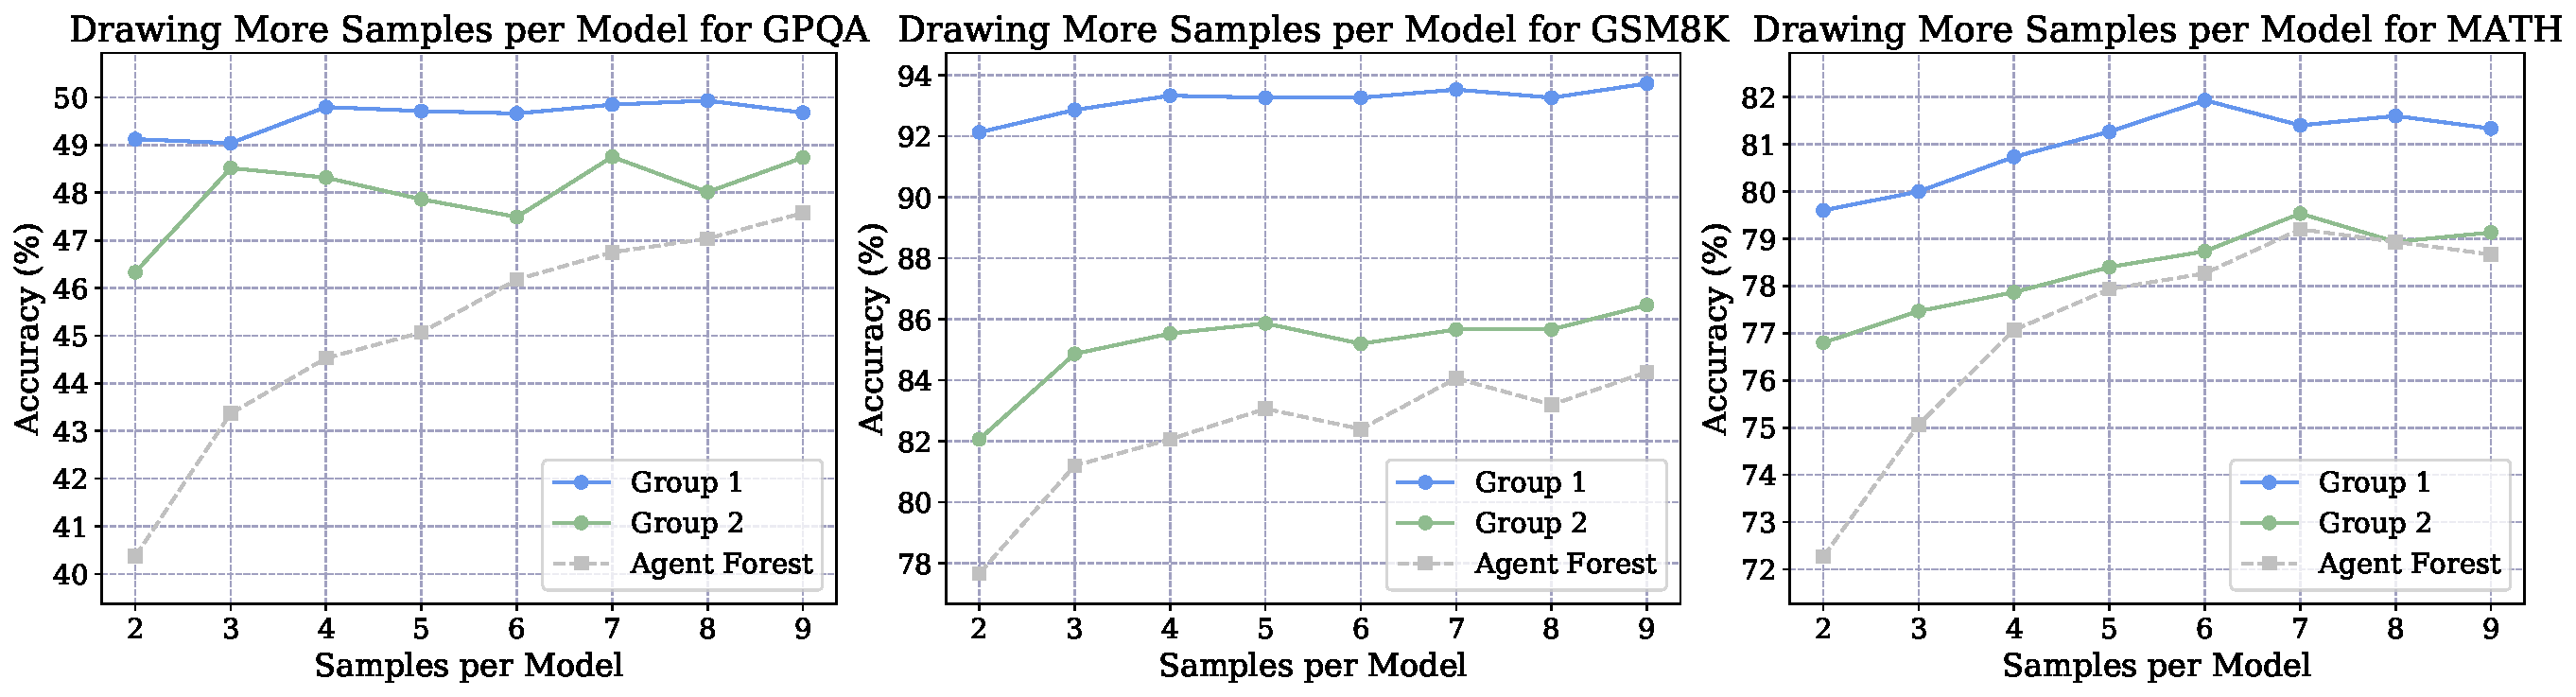
\includegraphics[width=\textwidth]{Figures/scaling_curves.pdf}
    \vspace{-20pt}
    \caption{\small \textbf{Drawing More Samples per Model Improves Accuracy}. We report mean accuracy of \NAME{} as the number of samples per model increases from 2 to 9 across three benchmarks. Group 1 and Group 2 are from  Table~\ref{tab:composition_results_combined}. We also plotted the mean accuracy of Agent Forest~\citep{li2024agentsneed} in grey line. }
    \vspace{-15pt}
    \label{fig:samples_per_model}
\end{figure}

\begin{figure}[t]
    \centering
    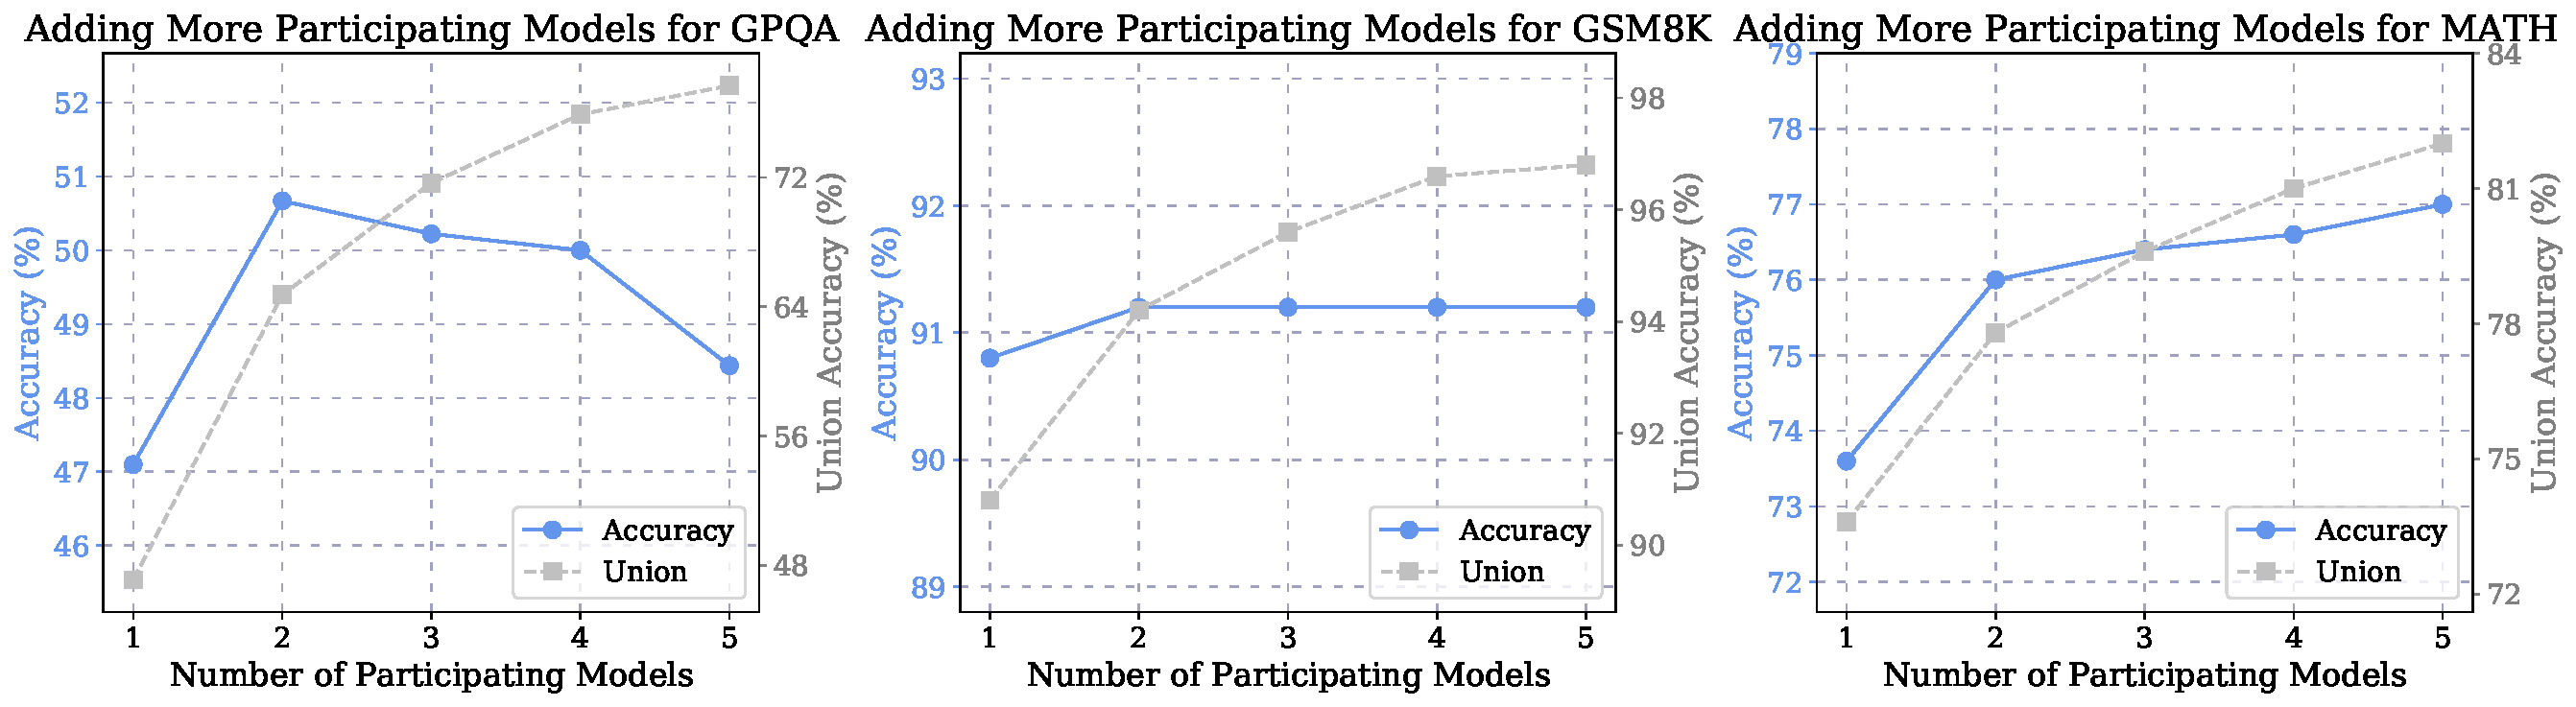
\includegraphics[width=\textwidth]{Figures/Adding_More_Participating_Models.pdf}
    \vspace{-20pt}
    \caption{\small \textbf{Adding More Participating Models Affects Accuracy Differently}. We report the mean accuracy (blue line) of the optimal \NAME{}  obtained when using 2 to 5 models across three benchmarks. We also report the union accuracy (grey line), defined in Section~\ref{sub:method-search}. The blue line (Mean Accuracy) is plotted against the left-hand Y-axis. The grey line (Union Accuracy) is plotted against the right-hand Y-axis. }
    % \vspace{-5pt}
    \label{fig:scaling_model_counts}
\end{figure}

% \begin{table}[htbp]
% \centering

% \small
% \begin{tabular}{l@{\hspace{2em}}cc@{\hspace{2em}}cc}
% \toprule
% \multirow{2}{*}{\textbf{Benchmark}} & \multicolumn{2}{c}{\textbf{Group 1}} & \multicolumn{2}{c}{\textbf{Group 2}} \\
% \cmidrule(lr){2-3} \cmidrule(lr){4-5}
% & \begin{tabular}[c]{@{}c@{}}Acc. \% \end{tabular} & \begin{tabular}[c]{@{}c@{}}$\Delta$ (Gain)\end{tabular} & \begin{tabular}[c]{@{}c@{}}Acc. \% \end{tabular} & \begin{tabular}[c]{@{}c@{}}$\Delta$ (Gain)\end{tabular} \\
% \midrule
% MATH & $81.9 \pm 0.2$ & $+6.4$ & $79.5 \pm 0.4$ & $+4.0$ \\
% GPQA & $49.9 \pm 1.8$ & $+4.8$ & $48.7 \pm 1.2$ & $+3.6$ \\
% GSM8K & $93.7 \pm 0.2$ & $+5.2$ & $86.5 \pm 0.8$ & $+5.7$ \\
% \bottomrule

% \end{tabular}
% \caption{\textbf{Best Accuracy after Sample Scaling} Acc indicates the highest accuracy achieved through scaling. Groups 1 \& 2 are defined in Table~\ref{tab:composition_results_combined}. Gain represents the improvement over the best single-model accuracy reported in Table~\ref{tab:composition_results_combined}.}
% \label{tab:scaling_best}
% \end{table}


\begin{table}[h]
\centering
\vspace{-10pt}
\setlength{\tabcolsep}{15pt}
\renewcommand{\arraystretch}{1.0}
\resizebox{\textwidth}{!}{
\small
\begin{tabular}{l@{\hspace{2em}}cc@{\hspace{2em}}cc@{\hspace{2em}}c}
\toprule
\multirow{2}{*}{\textbf{Benchmark}} & \multicolumn{2}{c}{\textbf{Group 1}} & \multicolumn{2}{c}{\textbf{Group 2}} & \multirow{2}{*}{\textbf{Qwen-2.5 72B Acc. \%}} \\
\cmidrule(lr){2-3} \cmidrule(lr){4-5}
& Acc. \% & $\Delta$ (Gain) & Acc. \% & $\Delta$ (Gain) &  \\
\midrule
MATH  & $81.9 \pm 0.2$ & $+6.4$ & $79.5 \pm 0.4$ & $+4.0$ & $82.3 \pm 0.5$ \\
GPQA  & $49.9 \pm 1.8$ & $+4.8$ & $48.7 \pm 1.2$ & $+3.6$ & $44.9 \pm 0.5$ \\
GSM8K & $93.7 \pm 0.2$ & $+5.2$ & $86.5 \pm 0.8$ & $+5.7$ & $90.4 \pm 0.3 $ \\
\bottomrule
\end{tabular}
}
\vspace{-5pt}
\caption{\textbf{Best Accuracy after Sample Scaling beats Larger Model.} 
Acc indicates the highest accuracy achieved through scaling. 
Groups 1 \& 2 are defined in Table~\ref{tab:composition_results_combined}. 
Gain represents the improvement over the best single-model accuracy reported in Table~\ref{tab:composition_results_combined}. 
For reference, we also include the performance of the large model Qwen-2.5 72B, showing that our composed small models can outperform it on GPQA and GSM8K.}
\label{tab:scaling_vs_qwen}
\vspace{-10pt
}
\end{table}



% \begin{table}[t]
% \centering
% \caption{Accuracy (\%) of different models on sampled questions from MATH, MMLU, GPQA, and GSM8K. 
% Each result is averaged over 3 runs (temperature = 0.5).\cw{This table should be put into appendix.}}
% \label{tab:exp_results}
% \resizebox{\textwidth}{!}{
% \begin{tabular}{lccccccc}
% \toprule
% Dataset & Gemma 2 27B & Qwen2.5-3B & Llama 3.2 3B & Llama 3.1 8B & Mistral Small 24B & Mixtral 8$\times$7B v0.1 & Qwen2.5-7B \\
% \midrule
% MATH   & $62.0 \pm 0.0$ & $51.0 \pm 2.0$ & $51.3 \pm 2.1$ & $50.3 \pm 1.5$ & $70.0 \pm 2.6$ & $34.0 \pm 3.5$ & $74.0 \pm 2.6$ \\
% MMLU   & $76.7 \pm 0.6$ & $35.0 \pm 5.6$ & $53.0 \pm 1.0$ & $57.3 \pm 2.1$ & $72.3 \pm 1.2$ & $62.3 \pm 1.5$ & $71.0 \pm 1.0$ \\
% GPQA   &  --  &  --  &  --  &  --  &  --  &  --  &  --  \\
% GSM8K  &  --  &  --  &  --  &  --  &  --  &  --  &  --  \\
% \midrule
% Average &  --  &  --  &  --  &  --  &  --  &  --  &  --  \\
% \bottomrule
% \end{tabular}
% }
% \label{tab:search_single_acc}
% \end{table}

% \subsection{Heterogeneous Instruction Tuning}

% \begin{table}[t]
%   \centering
%   \footnotesize
  
 
%   \begin{tabular}{lrrrr}
%     \toprule
%     \textbf{Method} & \textbf{Acc (\%)} & \textbf{$\Delta$ Acc (\%)} &
%     \textbf{Token Usage} & \textbf{$\Delta$ Tokens (\%)} \\
%     \midrule
%     Mixture-of-Agents                   & 58.6 & --   &   720,843  & --    \\
%     Mixture-of-Agents (w/ \NAME{})          & 59.6 & +1.0 &   595,269  & -17.4 \\
%     \midrule
%     LLM-Debate                          & 65.6 & --   & 1,960,680  & --    \\
%     LLM-Debate (w/ \NAME{})                 & 61.1 & -4.5 &   786,841  & -59.9 \\
%     \midrule
%     Multi-Agent Verification            & 64.2 & --   & 5,318,019  & --    \\
%     Multi-Agent Verification (w/ \NAME{})   & 61.6 & -2.6 & 1,249,373  & -76.5 \\
%     \midrule
%     \NAME{} (k=1)                           & 60.6 & --   &   581,498  & --    \\
%     \NAME{} (k=3)                           & \textbf{68.2} & --   & 1,509,557  & --    \\
%     \midrule
%     Upper Bound                         & 78.3 & --   &   --  & --    \\
%     \bottomrule
%   \end{tabular}
%   \vspace{5pt}
%   \caption{\small \textbf{\NAME{} Improves Computational Efficiency on GPQA.} Performance and computational efficiency of compositional methods on the GPQA dataset. 
%            "$\Delta$ Acc (\%)" indicates the accuracy difference achieved by the \NAME{} variant compared to
%            the original method, and "$\Delta$ Tokens (\%)" gives the relative token-usage reduction.}
%     \label{tab:composition-gpqa}
%     \vspace{-10pt}
% \end{table}
% % \vspace{-10pt}







% \section{Mathematical Analysis}
% \label{sect:analysis}

\paragraph{Comparative Analysis of \NAME{} and Other Voting-Based Composition Methods} As shown in Section~\ref{sect:experiment}, the \NAME{}  outperforms standard self-consistency~\citep{wang2023selfconsistencyimproveschainthought} and Agent Forest~\citep{li2024agentsneed}. Since our method also involves voting on model outputs, we examine its differences from these approaches to better explain the source of our improvements.

To explain our stronger performance, we note a limitation of self-consistency methods. Suppose a model has probability $p$ of answering a question correctly. When self-consistency samples $N$ responses, the probability of obtaining the correct answer after aggregation follows a binomial distribution.
% 
\begin{equation}
A(N, p) = \Pr\left( X \geq \left\lceil \tfrac{N}{2} \right\rceil \right) = \sum_{k=\lceil N/2 \rceil}^{N} \binom{N}{k} p^{k}(1-p)^{N-k}, \quad X \sim \text{Binomial}(N,p)
\end{equation}
% 
We observe that $A(N,p)$ exceeds $p$ only when $p > 0.5$, meaning self-consistency is effective only in this regime. When $p < 0.5$, however, self-consistency can actually lower overall accuracy.

For any dataset, we can conceptually divide examples into three types of questions. Type 1 includes cases where $p = 100\%$, so the LLM always answers correctly. Type 2 covers cases where $p > 50\%$, meaning the model is more likely than not to be correct. Type 3 includes cases where $p < 50\%$, where the model is more likely to be wrong. The overall effect of self-consistency is then the improvement from Type 2, offset by the degradation from Type 3. Improvement occurs only when the dataset contains a sufficiently large proportion of Type 2 questions. 

For the \NAME{}, we select the output from the most confident model, so the accuracy can be approximated as $A(N, p_{\max})$, where $p_{\max}$ is the highest probability among the three models. By increasing $p_{\max}$, we effectively enlarge the proportion of Type 2 questions, leading to higher overall accuracy.


For the Agent Forest approach, answers are drawn evenly from all models, so its accuracy can be approximated as $A(N, \bar{p})$, where $\bar{p}$ is the average probability across models. This generally results in lower accuracy than \NAME{}.



% \paragraph{Limitations and Future Work} 
% \label{subsec:method_limitation}
% Our proposed method has several limitations. First, PBC approach operates purely at inference time without any additional training, preventing us from fully exploiting the information in each language model. Future work could explore fine-tuning models jointly to fully combine information in models. In addition, PBC relies on generating multiple answers from a model as its estimated confidence, which can still be computationally expensive. Future work on more directly and more accurately estimating the confidence of a language model can greatly improve the efficiency and accuracy of the system.

% \cw{High level idea: This section, we need to analyze the failure of existing combination methods such as LLM debate on small models}




% \subsection{Composing Small-Scale Language Models}
% \label{subsec:method_pbc}

% \vspace{-5pt}
\vspace{-5pt}
\section{Discussion}
\vspace{3pt}
% \vspace{-3pt}
\label{sect:conclusion}
\vspace{-5pt}
\paragraph{Mathematical Analysis} 

% As shown in Section~\ref{sect:experiment}, the \NAME{}  outperforms standard self-consistency~\citep{wang2023selfconsistencyimproveschainthought} and Agent Forest~\citep{li2024agentsneed}. Since our method also involves voting on model outputs, we examine its differences from these approaches to better explain the source of our improvements.

\looseness=-1
To explain our good performance, we note a limitation of self-consistency methods. Suppose a model has probability $p$ of answering a question correctly. When self-consistency samples $N$ responses, the probability of obtaining the correct answer after aggregation follows a binomial distribution.
% 
\begin{equation*}
A(N, p) = \Pr\left( X \geq \left\lceil \tfrac{N}{2} \right\rceil \right) = \sum_{k=\lceil N/2 \rceil}^{N} \binom{N}{k} p^{k}(1-p)^{N-k}, \quad X \sim \text{Binomial}(N,p)
\end{equation*}
% 
$A(N,p)$ exceeds $p$ only when $p > 0.5$, meaning self-consistency is effective only in this regime. When $p < 0.5$, however, self-consistency can actually lower overall accuracy. For any dataset, we can conceptually divide examples into three types of questions. Type 1 includes cases where $p = 100\%$, so the LLM always answers correctly. Type 2 covers cases where $p > 50\%$, meaning the model is more likely than not to be correct. Type 3 includes cases where $p < 50\%$, where the model is more likely to be wrong. The overall effect of self-consistency is then the improvement from Type 2, offset by the degradation from Type 3. Improvement occurs only when the dataset contains a sufficiently large proportion of Type 2 questions. 

For the \NAME{}, we select the output from the most confident model, so the accuracy can be approximated as $A(N, p_{\max})$, where $p_{\max}$ is the highest probability among the three models. By increasing $p_{\max}$, we effectively enlarge the proportion of Type 2 questions, leading to higher overall accuracy. For the Agent Forest approach, answers are drawn evenly from all models, so its accuracy can be approximated as $A(N, \bar{p})$, where $\bar{p}$ is the average probability across models. This generally results in lower accuracy than \NAME{}.

\paragraph{Limitation and Future Work} The SLM-MUX framework has two main limitations. First, its design is static and does not adapt to specific questions. For every query, it uses a fixed group of models that are pre-selected through exhaustive search -- a method that is slow and costly when there are many models to choose from. When models are tied, the framework uses their past accuracy on a validation set to decide, which is also a fixed, non-adaptive rule. Second, the way the framework measures model confidence is simple. It relies only on self-consistency -- how often a model produces the same answer. This can be a problem because a model can be very consistent while still being incorrect.


\paragraph{Conclusion} 
This work demonstrates that orchestration methods designed for frontier models paradoxically degrade the performance of SLMs by amplifying errors. To address this, we propose \NAME{}, a framework that avoids inter-model discussion, instead selecting the most reliable output based on each model's self-consistency. We further introduce a model selection search algorithm to find complementary model combinations. Experiments show our method not only substantially outperforms existing strategies but also enables an ensemble of just two SLMs to surpass the much larger Qwen-2.5 72B model on key reasoning benchmarks. In summary, our work validates that intelligently orchestrating multiple efficient models—a "multi-core" approach—is a highly promising alternative to endlessly scaling monolithic models on the path toward more capable AI systems.

% Our paper studies how to effectively combine multiple language models together. We first identify some key reasons behind the limitations of existing compositional methods when applied to smaller-scale language models and introduce Protocol-Based Composition (PBC), an efficient, rule-based compositional method. Experimental results demonstrate that PBC significantly enhances the accuracy of small-scale language models and can also effectively integrate with state-of-the-art large-scale models, substantially reducing computational costs and resource consumption. Overall, our work points to a future direction of efficient language model systems consisting of many specialized language models jointly forming predictions.


\section*{Acknowledgments}
We thank Prof. Tom Griffiths (Princeton University) for insightful technical discussions, which inspired our early exploration of our method.

\bibliographystyle{iclr2026_conference}
\bibliography{iclr2026_conference}

\appendix

\newpage

\section*{Appendix Overview}

% The appendix is organized as follows. Section~\ref{sec:visual} includes additional visual examples illustrating the workflow and effectiveness of the \NAME{} method across the MATH, GPQA, and GSM8K datasets. Section~\ref{supp_sec:std_error} provides a statistical analysis of standard errors to demonstrate the consistency of our experimental results. Section~\ref{sec:randomness} evaluates the robustness of \NAME{} against randomness introduced by varying the temperature settings. Section~\ref{sec:SLM-Mux-vs-majority} analyzes in detail why \NAME{} outperforms majority voting, especially on challenging problems. Section~\ref{sec:single-models} reports the accuracy results for individual models used in our experiments. Section~\ref{sec:licenses} provides the licensing details for the datasets. \cw{TODO update this}

The appendix is organized as follows. Section~\ref{sec:visual} presents additional visual examples illustrating the workflow and effectiveness of the \NAME{} method across the MATH, GPQA, and GSM8K datasets. Section~\ref{sec:slm-failure} provides a detailed analysis of SLM failures in discussion-based orchestration methods, drawing on experiment logs to highlight common failure patterns. Section~\ref{sec:single-models} reports the accuracy of individual models used in our experiments. Finally, Section~\ref{sec:licenses} provides the licensing details for the datasets.


\section{LLM Usage Statement}
\label{sec:usage}

We used Cursor for coding. Large language models (LLMs) were employed to help polish drafts written by humans, and to assist in searching for related papers. The final choice of related work included in this paper was made entirely by the human authors after careful screening. LLMs were also used for proofreading and for providing suggestions.

% \section{LLM Usage Statement}
% \label{sec:visual}


\section{Additional Visual Illustrations of \NAME{}}
\label{sec:visual}

To more effectively illustrate the workflow of our proposed composition method, we select several representative examples from the logs. We demonstrate them in Figure~\ref{fig:example_1}, Figure~\ref{fig:example_2} and Figure~\ref{fig:example_3}.

\paragraph{\NAME{} surpasses majority voting in scenarios with initial disagreement among models.} As illustrated by Figure~\ref{fig:example_1}, during the independent generation phase, Gemma-2-27B is the sole model to provide the correct answer. Hence, majority voting applied directly would fail to select the correct author. 


\begin{figure}[ht]
    \centering
    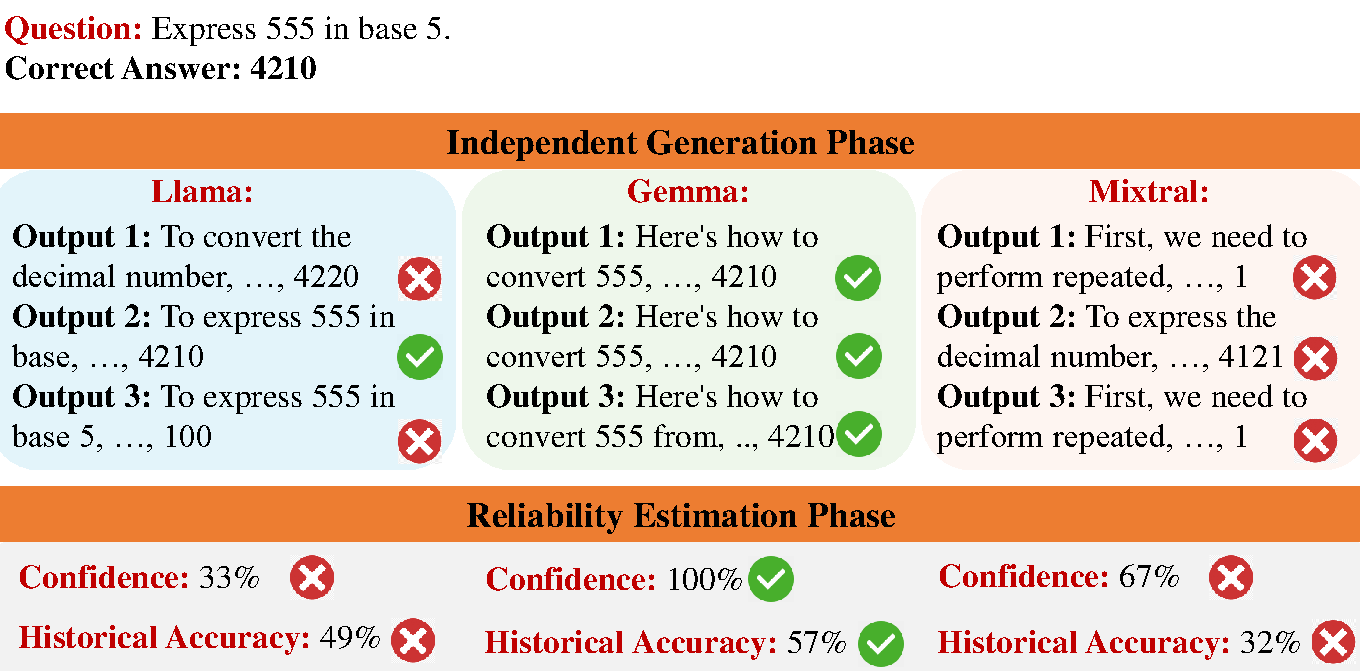
\includegraphics[width=0.7\linewidth]{Figures/example_1_cropped.pdf}
    \caption{\textbf{An illustration of the \NAME{} method applied to the MATH dataset.} In the independent generation phase, three models are used: LLaMA-3.1-8B (denoted as Llama), Gemma-2-27B (denoted as Gemma), and Mixtral-8$\times$7B (denoted as Mixtral). Because the three models provide different answers at first, so each model is invoked two more times. Gemma obtains the highest confidence score and is therefore selected as the final output.}
    \label{fig:example_1}
\end{figure}

\begin{figure}[ht]
    \centering
    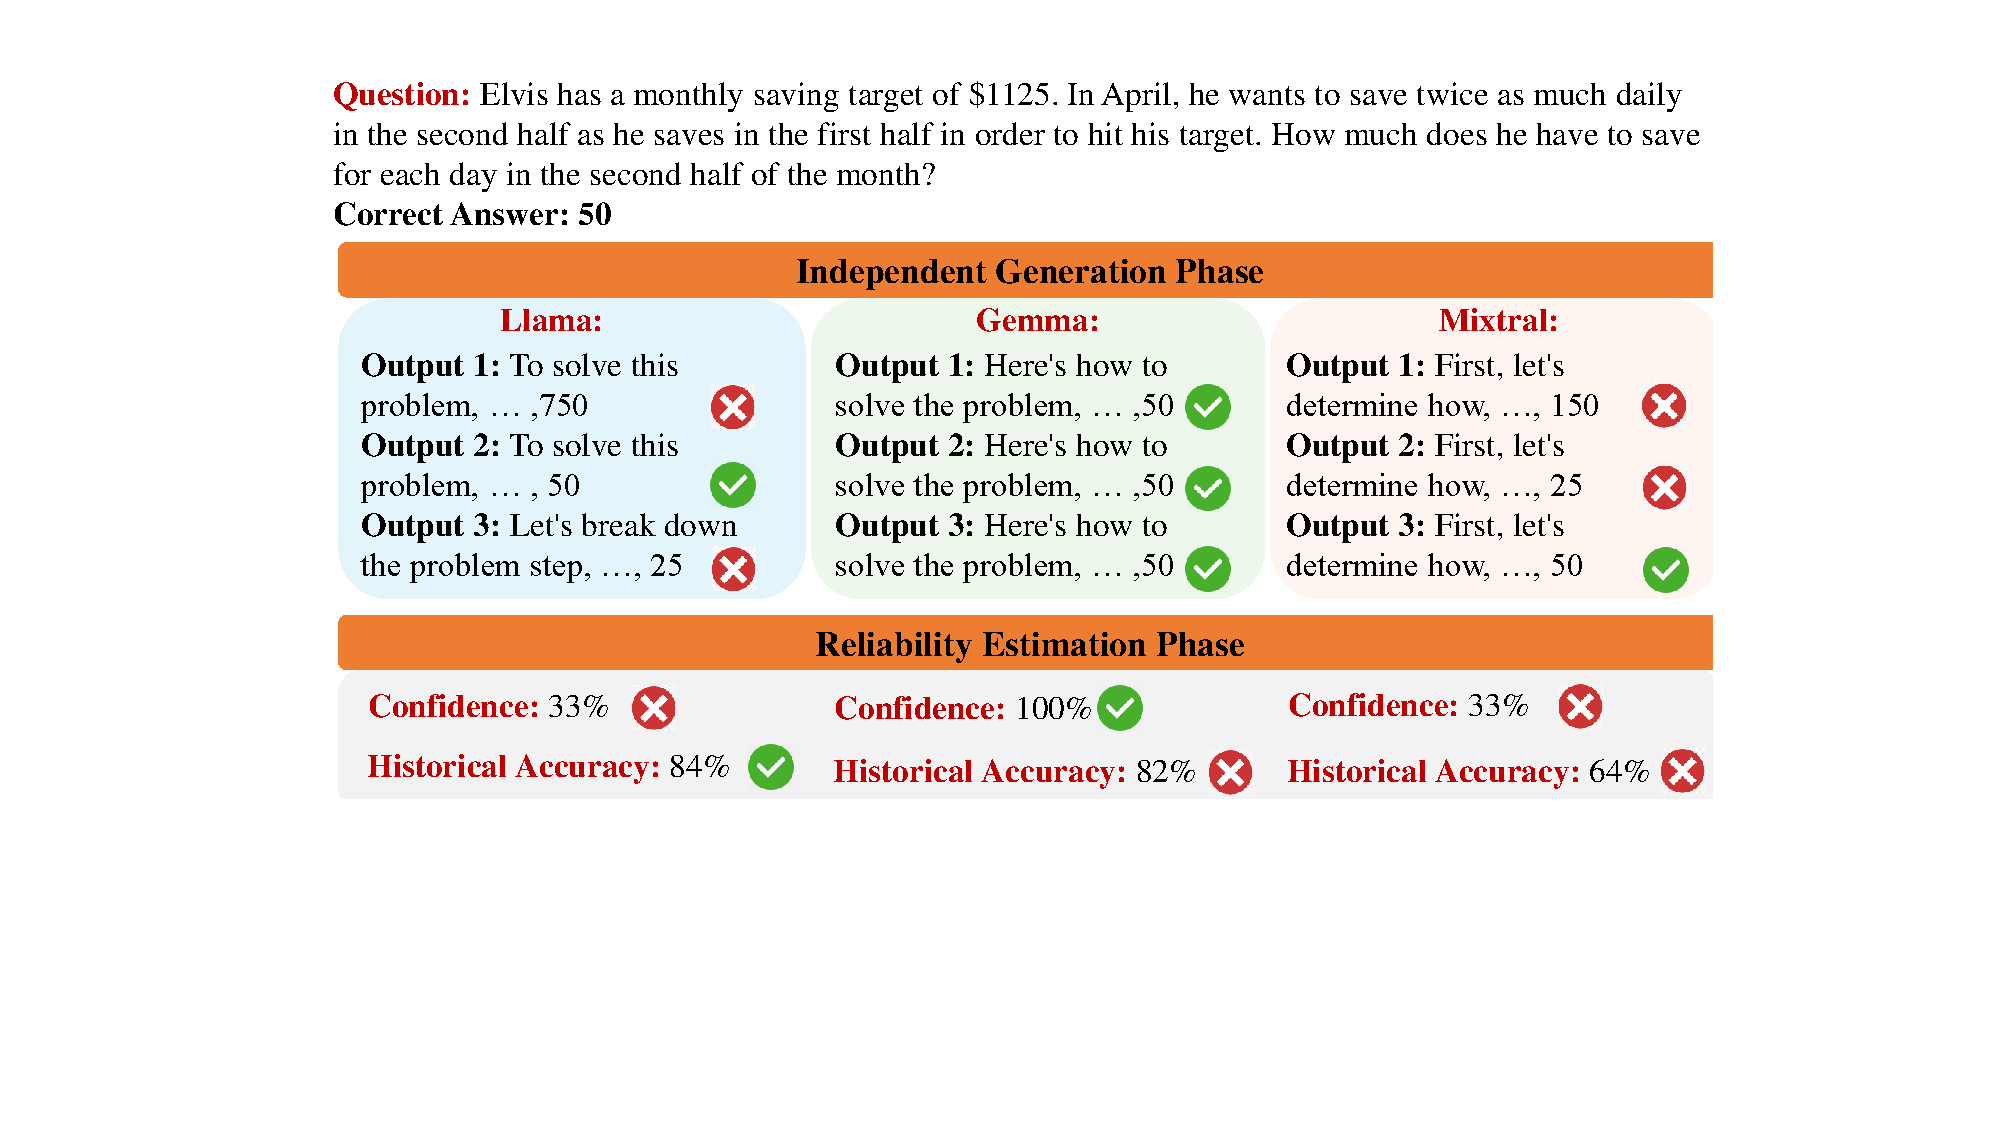
\includegraphics[width=0.7\linewidth]{Figures/example_2_cropped.pdf}
    \caption{\textbf{An illustration of the \NAME{} method applied to the GSM8K dataset.} In the independent generation phase, different models produce different answers. However, when we invoke each model multiple times, we observe that Llama and Mixtral only yield correct answers approximately one-third of the time. In contrast, Gemma demonstrates stable performance.}
    \label{fig:example_2}
\end{figure}

\begin{figure}[ht]
    \centering
    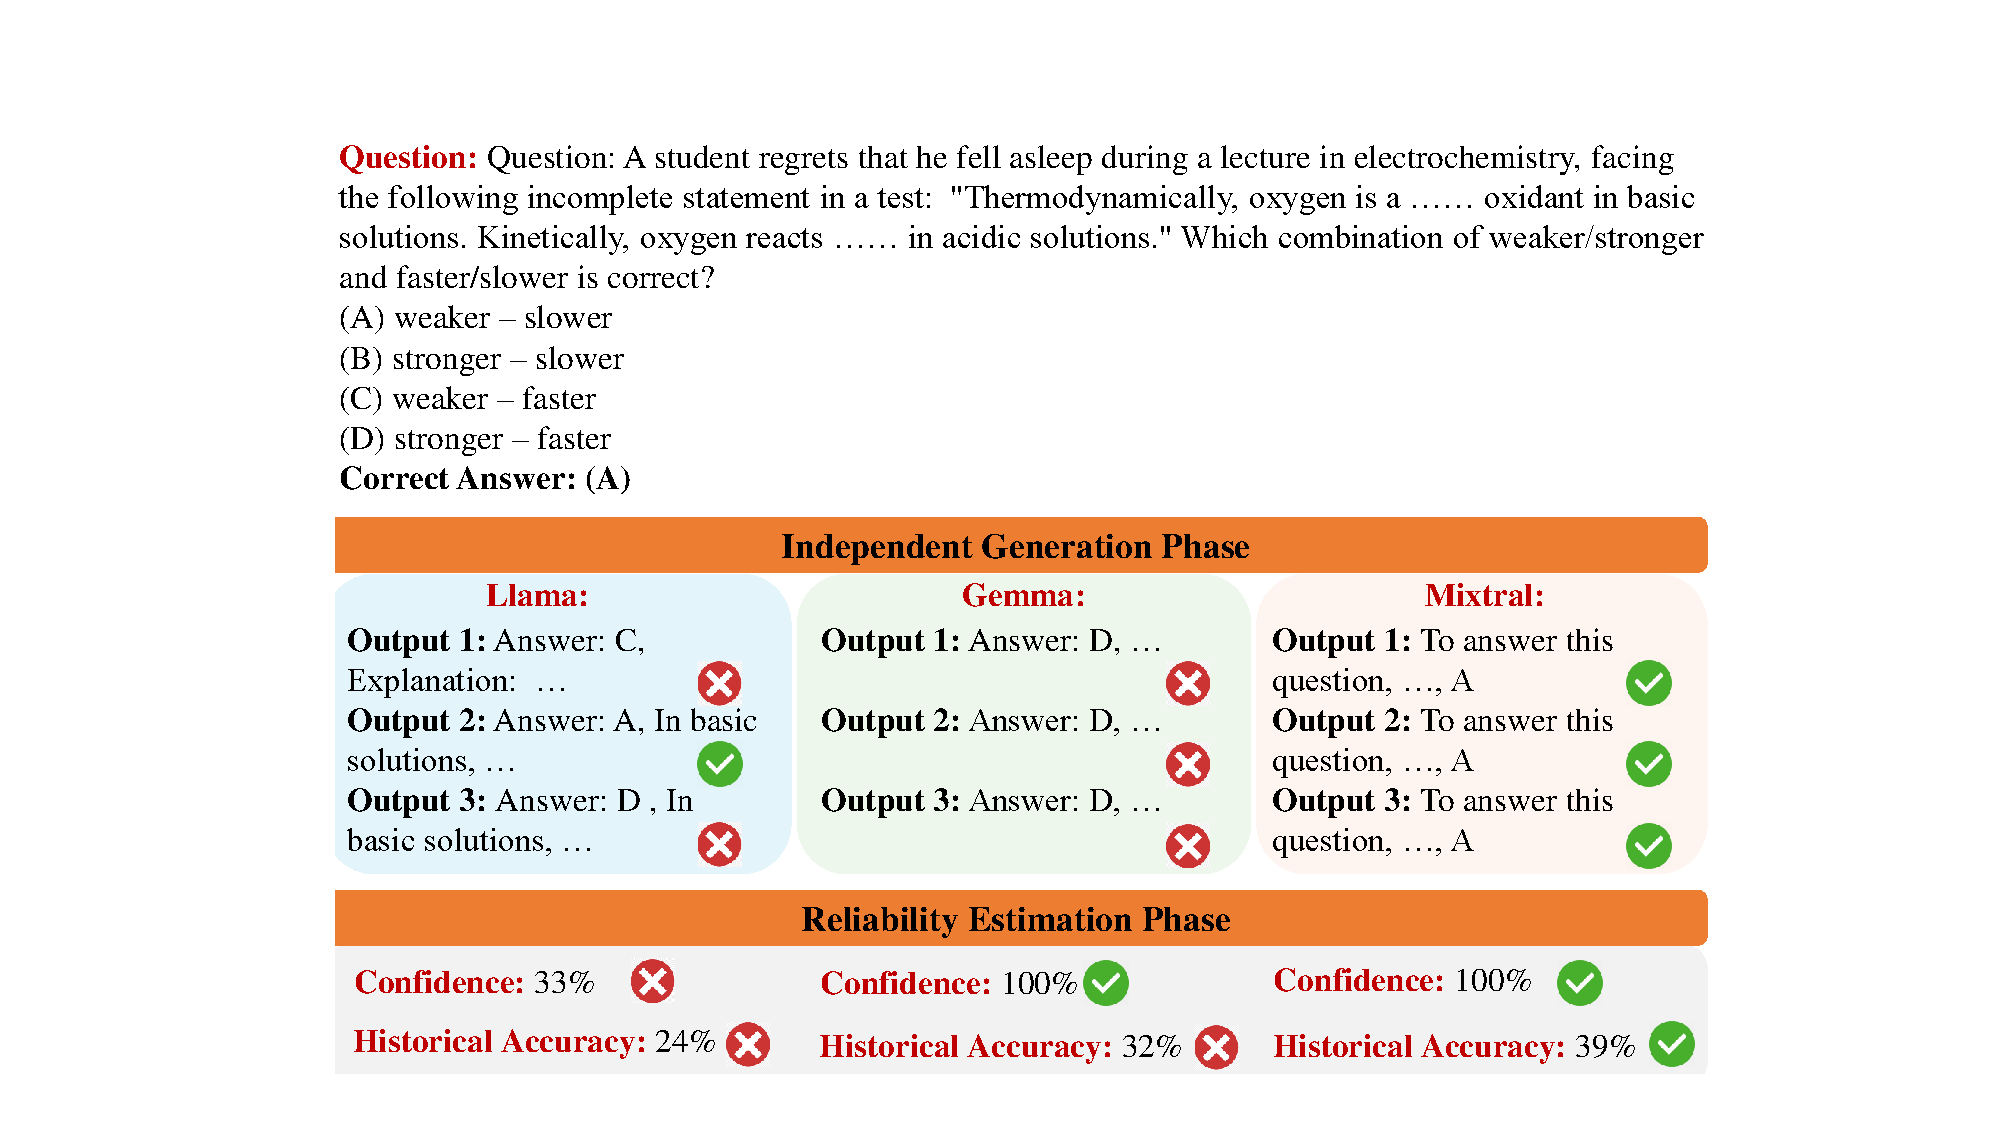
\includegraphics[width=0.7\linewidth]{Figures/example_3_cropped.pdf}
    \caption{\textbf{An illustration of the \NAME{} method applied to the GPQA dataset.} During the independent generation phase, Gemma and Mixtral obtain the same confidence score. However, considering historical accuracy, Mixtral ranks higher. Therefore, Mixtral's answer is selected as the final output.}
    \label{fig:example_3}
\end{figure}



% \section{Analyzing Standard Error in Results}
% \label{supp_sec:std_error}
% To support our primary claim that the proposed method yields a significant improvement in accuracy (as shown in Table~\ref{tab:composition-combined}), we further analyze the statistical significance in our experimental results. Specifically, we analyze logs from experiments and compute the standard error (standard deviation divided by the square root of the number of samples) across different samples. The results of this analysis are presented in Table~\ref{tab:SLM-Mux-results-se}. We observe that the standard error associated with our method is relatively small, indicating consistency and reliability in benchmark performance. 

% To quantify the uncertainty associated with our reported accuracies, we computed the standard error by treating the correctness of each response as an independent Bernoulli random variable. Specifically, for each item, we assign a binary value \( X_i \), where \( X_i = 1 \) indicates a correct response and \( X_i = 0 \) an incorrect one. Given an empirical accuracy \(\hat{p} = \frac{1}{n}\sum_{i=1}^{n} X_i\) computed over \(n\) samples, the standard error (SE) of this accuracy estimate is calculated as follows:

% \[
% \text{SE} = \sqrt{\frac{\hat{p}(1 - \hat{p})}{n}}.
% \]

% This standard error serves as the basis for the error bars presented in Table~\ref{tab:SLM-Mux-results-se}, reflecting the expected magnitude of sampling variability if the experiment were repeated under identical conditions.

% \begin{table}[ht]
% \centering
% \small
% \begin{tabular}{lccc}
% \toprule
% \textbf{Method} & \textbf{MATH Acc (\%)} & \textbf{GPQA Acc (\%)} & \textbf{GSM8K Acc (\%)} \\
% \midrule
% Mixture-of-Agents          & 51.4 $\pm$ 2.24 & 33.3 $\pm$ 3.37 & 81.6 $\pm$ 1.73 \\
% LLM-Debate                  & 51.6 $\pm$ 2.23 & 36.8 $\pm$ 3.44 & 80.8 $\pm$ 1.76 \\
% Multi-Agent Verification    & 48.4 $\pm$ 2.23 & 35.3 $\pm$ 3.41 & 86.4 $\pm$ 1.53 \\
% \textbf{\NAME{} (Ours)}         & \textbf{63.0 $\pm$ 2.16} & 41.9 $\pm$ 3.52 & \textbf{88.4 $\pm$ 1.43} \\
% \midrule
% Single-Best                 & 56.8 $\pm$ 2.22 & 38.9 $\pm$ 3.48 & 84.2 $\pm$ 1.63 \\
% Single-Best-SC              & 58.0 $\pm$ 2.21 & \textbf{42.4 $\pm$ 3.53} & 86.8 $\pm$ 1.51 \\
% Upper Bound                 & 64.6 $\pm$ 2.14 & 57.0 $\pm$ 3.54 & 92.0 $\pm$ 1.21 \\
% \bottomrule
% \end{tabular}
% % \vspace{5pt}
% \caption{\small \textbf{Accuracy with Standard Error.} The standard error across MATH, GPQA, and GSM8K for various methods. \NAME{} demonstrates relatively small standard errors.}
% \label{tab:SLM-Mux-results-se}
% % \vspace{-5pt}
% \end{table}


% \section{Analyzing Randomness in Results}
% \label{sec:randomness}
% Given that our method incorporates stochasticity solely through temperature settings greater than zero, we conducted additional experiments to explicitly quantify the randomness introduced by varying temperature values. The results, summarized in Table~\ref{tab:SLM-Mux-results-temp}, demonstrate that our approach exhibits strong robustness with respect to temperature-induced variability.

% \begin{table}[htbp]
% \centering
% \small
% \begin{tabular}{lccc}
% \toprule
% \textbf{Method} & \textbf{MATH Acc (\%)} & \textbf{GPQA Acc (\%)} & \textbf{GSM8K Acc (\%)} \\
% \midrule
% \textbf{\NAME{} (Ours)} & 61.8 $\pm$ 1.2 & 42.1 $\pm$ 0.3 & 87.8 $\pm$ 0.6 \\
% \bottomrule
% \end{tabular}
% \vspace{5pt}
% \caption{\small \textbf{Accuracy with Temperature-error bars of \NAME{} Method.}}
% \label{tab:SLM-Mux-results-temp}
% \end{table}




% \section{Analysis on Why \NAME{} Outperforms Majority Voting Methods like Agent Forest}
% \label{sec:SLM-Mux-vs-majority}

% Majority voting only improves accuracy for simpler tasks. Our experimental results indicate that majority voting enhances accuracy solely when applied to simple questions, and it does not outperform the best individual LLM prediction for complex problems. Through detailed analysis, we observed that for simpler questions, disagreements among individual LLM predictions are typically limited, whereas for complex problems, such disagreements become significantly pronounced. We model this problem by assuming each LLM independently generates answers, where each answer has a probability \( p \) of being correct. Under this assumption, the theoretical accuracy \( A(N, p) \) achievable by majority voting among \( N \) independently predicting models is described by the cumulative probability of a binomial distribution:

% \begin{equation}
% A(N, p) = \Pr\left(X \ge \left\lceil \frac{N}{2} \right\rceil\right) = \sum_{k=\lceil \frac{N}{2} \rceil}^{N} \binom{N}{k} p^{k}(1 - p)^{N - k}, \quad X \sim \text{Binomial}(N, p)
% \end{equation}

% % Placeholder for composed accuracy figure
% \begin{figure}[ht]
%     \centering
%     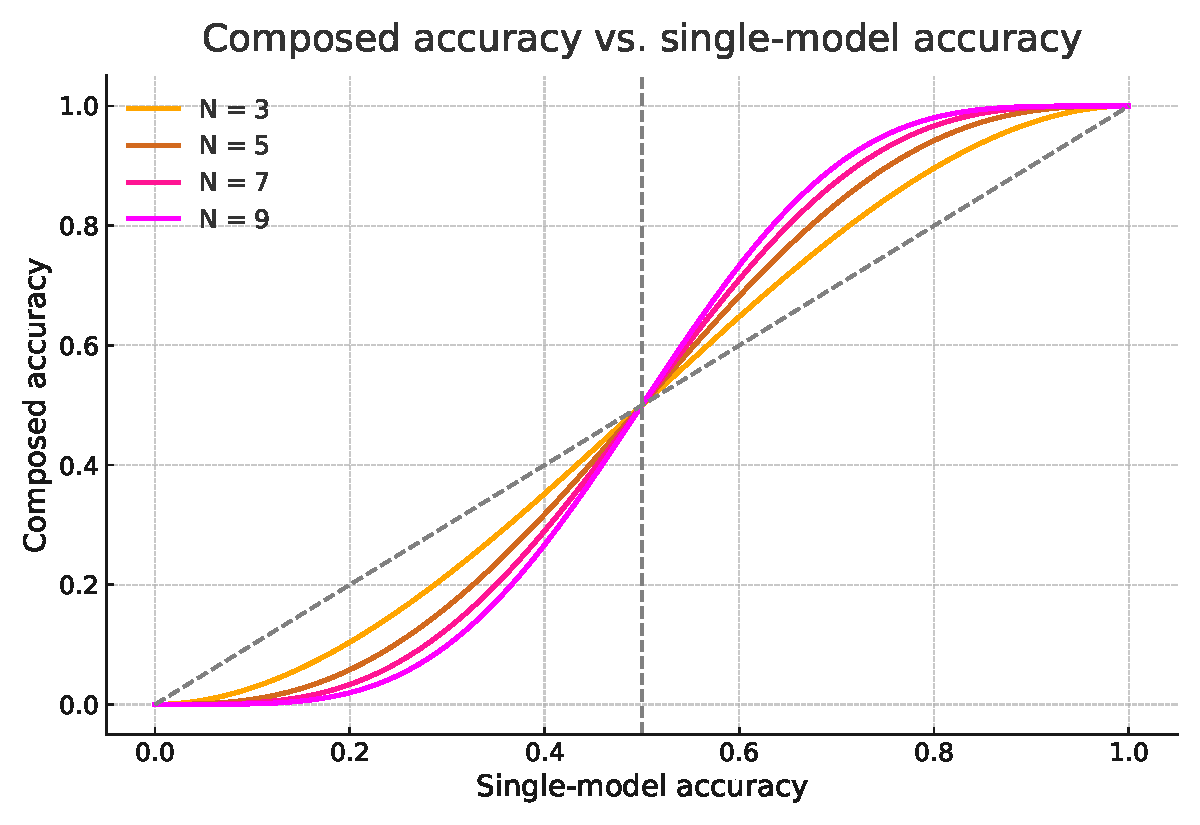
\includegraphics[width=0.7\linewidth]{Figures/composed_accuracy.pdf}
%     \caption{\textbf{Compared with Composed Accuracy and Single-model Accuracy.} Theoretical composed accuracy $A(N, p)$ as a function of individual accuracy $p$ for different numbers of models ($N = 3, 5, 7, 9$).}
%     \label{fig:composed_accuracy}
% \end{figure}

% In Figure~\ref{fig:composed_accuracy}, we plot the theoretical accuracy \( A(N, p) \) as a function of individual accuracy \( p \) for different numbers of models (\( N = 3, 5, 7, 9 \)). This plot clearly demonstrates that composed accuracy \( A(N, p) \) surpasses individual accuracy \( p \) only when \( p > 0.5 \). Conversely, for values of \( p \leq 0.5 \), majority voting negatively impacts performance, indicating that aggregation is counterproductive when individual models perform near or below chance.

% When multiple LLMs with varying accuracies participate in a simple majority vote, those with lower accuracy (close to or below chance level, i.e., $\leq 0.5$) can substantially dilute the contribution of higher-performing models. Essentially, the errors made by lower-accuracy models may dominate the voting outcome, pulling down the overall accuracy rather than enhancing it.

% In contrast, \NAME{} addresses this limitation by first evaluating each model’s consistency and confidence internally through multiple self-sampled predictions. Models that fail to demonstrate consistent confidence in their answers are filtered out, ensuring only the predictions from reliable, higher-performing models contribute significantly to the final decision. Furthermore, \NAME{} employs historical accuracy records of each model as prior knowledge to weight decisions effectively, further enhancing its ability to select the optimal predictions.

% Thus, while majority voting indiscriminately aggregates predictions, potentially amplifying errors from weaker models, \NAME{} selectively incorporates predictions, significantly improving accuracy, particularly in challenging scenarios.

% \section{Situations in Which \NAME{} is Less Effective}
% \label{{sec:SLM-Mux-less-effective}}


\section{Detailed Analysis of SLM Failures in Discussion-Based Methods}
\label{sec:slm-failure}

% We analyze the experiment logs of LLM-Debate when using SLMs, specifically the one presented in Section~\ref{sec:comparison}.
% This file contains 242 failure debate logs out of 500. We first prompt another analyzer LLM to analyze the reason for the failure; after we get the 242 analyses generated by the analyzer LLM, we then prompted another LLM, we then prompted another LLM to label the logs whterh they are failed due to groupthinking. We get 16? of our 242 labeled as yes. Which reinforce our statement. 

% The prompt in the analyzor LLMs and labelor aredemonstrated in box below


We analyze the experiment logs of LLM-Debate using small language models (SLMs) in Section~\ref{sec:comparison}. Among 500 debate problems, 242 resulted in failure (48.4\%). For each of the 242 failed debates, we first used an analyzer LLM to produce a process-focused failure analysis. We then used a separate labeling LLM to classify whether each failed debate was due to groupthink.


The labeling results are shown in Table~\ref{tab:label}:

\begin{table}[t]
\centering
\begin{tabular}{@{}l r l@{}}
\toprule
Metric & Count & Rate \\
\midrule
Total Debates Analyzed & 500 & 100\% of total \\
Failed Debates (System Error) & 242 & 48.4\% of total \\
\midrule
\multicolumn{3}{@{}l}{\textit{Breakdown of Failed Debates:}} \\
\quad Attributed to Groupthink & 144 & 59.5\% of failures \\
\quad Attributed to Other Causes & 79 & 32.6\% of failures \\
\quad Classification Unsuccessful & 19 & 7.9\% of failures \\
\bottomrule
\end{tabular}
\caption{\textbf{Failure Cause Attribution} This table shows the cause attribution for LLM-Debate when involving SLMs.}
\label{tab:label}
\end{table}

These results reinforce our claim that groupthink is a major failure mode in SLM-based LLM-debate.

We provide the exact prompts used by (i) the analyzer LLM to generate the 242 failure analyses (Figure~\ref{lst:prompt-analyzer}) and (ii) the groupthink labeler LLM to classify groupthink (Figure~\ref{lst:prompt-groupthink-system}). Placeholders such as \texttt{\{problem\}} indicate runtime substitutions by our code.

% \noindent Source: \texttt{analyze\_incorrect\_problems.py} (function \texttt{create\_analysis\_prompt})
% (previous content above lstlisting)
\lstdefinestyle{promptstyle}{basicstyle=\ttfamily,breaklines=true,backgroundcolor=\color{gray!10}}

% \begin{minipage}{\linewidth}
% \begin{lstlisting}[style=promptstyle][style=promptstyle]
% As an expert in analyzing multi-agent AI systems, your task is to analyze why an 'LLM Debate' process failed to find the correct answer. Your focus should be on the *debate dynamics and process*, not just the mathematical details. The goal is to understand the failure of the debate methodology itself.

% **Ground Truth:**
% - **Problem Statement:** {problem}
% - **Correct Answer:** {ref_answer}

% **Debate Information:**
% - **Final Incorrect Answer from System:** {system_answer}

% **Analysis of Round 1:**
% - **Model `{model_name}` proposed:**
%   - Answer: `{extracted_answer}`
%   - Reasoning:
% ```
% {full_text}
% ```

% ... (repeats per round and per model)

% **Your Analysis Task:**
% Based on the debate history, provide a "Debate Failure Analysis". Do not focus on simple calculation mistakes. Instead, analyze the interaction between the models and the structure of the debate. Pinpoint the core reasons the *debate process* failed. Consider these questions:

% 1.  **Error Propagation vs. Correction:** How did initial errors influence later rounds? Were there moments where a correct idea was introduced but ignored or overruled? Why did the debate fail to self-correct?
% 2.  **Groupthink and Influence Dynamics:** Did the models converge on a flawed consensus? Did one or more influential but incorrect models lead the group astray? Was there evidence of independent reasoning that was shut down?
% 3.  **Argumentation Quality:** Did the models provide convincing but ultimately flawed arguments? Did they effectively challenge each other's reasoning, or was the debate superficial?
% 4.  **Critical Failure Point in the Debate:** Identify the single most critical turn or moment in the debate that sealed its failure. What happened, and why was it so impactful?
% 5.  **Improving the Debate:** What is the single most important change to the debate protocol or dynamics that could have prevented this failure? (e.g., different communication rules, promoting dissident opinions, etc.)

% Provide a concise, expert analysis focusing on the *process* failure.
% \end{lstlisting}
% \caption{Analyzer Prompt}
% \end{minipage}


\begin{figure}[htbp]
  \begin{minipage}{\linewidth}
  \begin{lstlisting}[style=promptstyle]
As an expert in analyzing multi-agent AI systems, your task is to analyze why an 'LLM Debate' process failed to find the correct answer. Your focus should be on the *debate dynamics and process*, not just the mathematical details. The goal is to understand the failure of the debate methodology itself.

**Ground Truth:**
- **Problem Statement:** {problem}
- **Correct Answer:** {ref_answer}

**Debate Information:**
- **Final Incorrect Answer from System:** {system_answer}

**Analysis of Round 1:**
- **Model `{model_name}` proposed:**
  - Answer: `{extracted_answer}`
  - Reasoning:
```
{full_text}
```

... (repeats per round and per model)

**Your Analysis Task:**
Based on the debate history, provide a "Debate Failure Analysis". Do not focus on simple calculation mistakes. Instead, analyze the interaction between the models and the structure of the debate. Pinpoint the core reasons the *debate process* failed. Consider these questions:

1.  **Error Propagation vs. Correction:** How did initial errors influence later rounds? Were there moments where a correct idea was introduced but ignored or overruled? Why did the debate fail to self-correct?
2.  **Groupthink and Influence Dynamics:** Did the models converge on a flawed consensus? Did one or more influential but incorrect models lead the group astray? Was there evidence of independent reasoning that was shut down?
3.  **Argumentation Quality:** Did the models provide convincing but ultimately flawed arguments? Did they effectively challenge each other's reasoning, or was the debate superficial?
4.  **Critical Failure Point in the Debate:** Identify the single most critical turn or moment in the debate that sealed its failure. What happened, and why was it so impactful?
5.  **Improving the Debate:** What is the single most important change to the debate protocol or dynamics that could have prevented this failure? (e.g., different communication rules, promoting dissident opinions, etc.)

Provide a concise, expert analysis focusing on the *process* failure.
\end{lstlisting}
  \end{minipage}
  \caption{Prompt Template for Failure Analysis.}
  \label{lst:prompt-analyzer}
\end{figure}

\begin{figure}[htbp]
  \begin{minipage}{\linewidth}
  \begin{lstlisting}[style=promptstyle]
You are an expert analyst of multi-agent LLM debates. Your goal is to determine whether the failure primarily involved groupthink/conformity dynamics. Groupthink indicators include: early flawed consensus, explicit capitulation to a majority, social proofing, adopting peers' answers without critique, abandoning independent reasoning to match others, or reinforcing an incorrect majority despite available dissent. Not-groupthink includes failures due to independent arithmetic/logic errors, argument complexity/veneer effects without convergence, or chaotic divergence with no consensus influence. Return STRICT JSON only, with keys: groupthink (bool), confidence (float 0-1), reasons (string), cues (array of strings).
\end{lstlisting}
  \end{minipage}
  \caption{Prompt for Groupthink Classification.}
  \label{lst:prompt-groupthink-system}
\end{figure}

\section{Accuracy of Single LLMs}
\label{sec:single-models}
We evaluated the accuracy of single model accuracy under the condition of temperature equal to zero. The results are shown in Table~\ref{tab:base-models-combined} and Table~\ref{tab:base-models}.

\begin{table}[hbtp]
\centering
\begin{tabular}{lccc}
\toprule
\textbf{Model} & \textbf{MATH Acc (\%)} & \textbf{GPQA Acc (\%)} & \textbf{GSM Acc (\%)} \\
\midrule
Llama-3.1-8B         & 48.6 & 23.7 & 84.2 \\
Mistral-8$\times$7B  & 31.6 & 31.9 & 63.4 \\
Gemma-2-27B          & 56.8 & 38.8 & 81.6 \\
\bottomrule
\end{tabular}
\vspace{5pt}
\caption{\textbf{Small Model Base Performance.} Base model accuracy on MATH, GPQA, and GSM8K.}
\label{tab:base-models-combined}
\end{table}


\begin{table}[hbtp]
\centering
\begin{tabular}{lcccc}
\toprule
\multirow{2}{*}{\textbf{Model}} & \multicolumn{2}{c}{\textbf{MATH}} & \multicolumn{2}{c}{\textbf{GPQA}} \\
\cmidrule(lr){2-3} \cmidrule(lr){4-5}
& \textbf{Accuracy (\%)} & \textbf{Token Usage} & \textbf{Accuracy (\%)} & \textbf{Token Usage} \\
\midrule
DeepSeek V3       & 87.0  & 419,513   & 55.1  & 173,885 \\
Gemini 2.0 Flash  & 90.4  & 361,737   & 63.6  & 195,576 \\
GPT-4o            & 79.8  & 408,410   & 51.0  & 212,037 \\
\bottomrule
\end{tabular}
\vspace{5pt}
\caption{\textbf{Large Model Base Performance.} Base model performance and token usage on MATH and GPQA datasets. Accuracy is the percentage of correct answers, and token usage reflects total tokens consumed (prompt + response) over the entire dataset for each model.}
\label{tab:base-models}
\vspace{-15pt}
\end{table}


\section{Licenses for Datasets}
\label{sec:licenses}
The MATH dataset is licensed under the MIT License.\\
The GPQA dataset is licensed under the Creative Commons Attribution 4.0 International (CC BY 4.0) License.\\
The GSM8K dataset is licensed under the MIT License.


\end{document}
% ================= Our paper content ends here =================

\section{Submission of conference papers to ICLR 2026}

ICLR requires electronic submissions, processed by
\url{https://openreview.net/}. See ICLR's website for more instructions.

If your paper is ultimately accepted, the statement {\tt
  {\textbackslash}iclrfinalcopy} should be inserted to adjust the
format to the camera ready requirements.

The format for the submissions is a variant of the NeurIPS format.
Please read carefully the instructions below, and follow them
faithfully.

\subsection{Style}

Papers to be submitted to ICLR 2026 must be prepared according to the
instructions presented here.

%% Please note that we have introduced automatic line number generation
%% into the style file for \LaTeXe. This is to help reviewers
%% refer to specific lines of the paper when they make their comments. Please do
%% NOT refer to these line numbers in your paper as they will be removed from the
%% style file for the final version of accepted papers.

Authors are required to use the ICLR \LaTeX{} style files obtainable at the
ICLR website. Please make sure you use the current files and
not previous versions. Tweaking the style files may be grounds for rejection.

\subsection{Retrieval of style files}

The style files for ICLR and other conference information are available online at:
\begin{center}
   \url{http://www.iclr.cc/}
\end{center}
The file \verb+iclr2026_conference.pdf+ contains these
instructions and illustrates the
various formatting requirements your ICLR paper must satisfy.
Submissions must be made using \LaTeX{} and the style files
\verb+iclr2026_conference.sty+ and \verb+iclr2026_conference.bst+ (to be used with \LaTeX{}2e). The file
\verb+iclr2026_conference.tex+ may be used as a ``shell'' for writing your paper. All you
have to do is replace the author, title, abstract, and text of the paper with
your own.

The formatting instructions contained in these style files are summarized in
sections \ref{gen_inst}, \ref{headings}, and \ref{others} below.

\section{General formatting instructions}
\label{gen_inst}

The text must be confined within a rectangle 5.5~inches (33~picas) wide and
9~inches (54~picas) long. The left margin is 1.5~inch (9~picas).
Use 10~point type with a vertical spacing of 11~points. Times New Roman is the
preferred typeface throughout. Paragraphs are separated by 1/2~line space,
with no indentation.

Paper title is 17~point, in small caps and left-aligned.
All pages should start at 1~inch (6~picas) from the top of the page.

Authors' names are
set in boldface, and each name is placed above its corresponding
address. The lead author's name is to be listed first, and
the co-authors' names are set to follow. Authors sharing the
same address can be on the same line.

Please pay special attention to the instructions in section \ref{others}
regarding figures, tables, acknowledgments, and references.


There will be a strict upper limit of 10 pages for the main text of the initial submission, with unlimited additional pages for citations. 

\section{Headings: first level}
\label{headings}

First level headings are in small caps,
flush left and in point size 12. One line space before the first level
heading and 1/2~line space after the first level heading.

\subsection{Headings: second level}

Second level headings are in small caps,
flush left and in point size 10. One line space before the second level
heading and 1/2~line space after the second level heading.

\subsubsection{Headings: third level}

Third level headings are in small caps,
flush left and in point size 10. One line space before the third level
heading and 1/2~line space after the third level heading.

\section{Citations, figures, tables, references}
\label{others}

These instructions apply to everyone, regardless of the formatter being used.

\subsection{Citations within the text}

Citations within the text should be based on the \texttt{natbib} package
and include the authors' last names and year (with the ``et~al.'' construct
for more than two authors). When the authors or the publication are
included in the sentence, the citation should not be in parenthesis using \verb|\citet{}| (as
in ``See \citet{Hinton06} for more information.''). Otherwise, the citation
should be in parenthesis using \verb|\citep{}| (as in ``Deep learning shows promise to make progress
towards AI~\citep{Bengio+chapter2007}.'').

The corresponding references are to be listed in alphabetical order of
authors, in the \textsc{References} section. As to the format of the
references themselves, any style is acceptable as long as it is used
consistently.

\subsection{Footnotes}

Indicate footnotes with a number\footnote{Sample of the first footnote} in the
text. Place the footnotes at the bottom of the page on which they appear.
Precede the footnote with a horizontal rule of 2~inches
(12~picas).\footnote{Sample of the second footnote}

\subsection{Figures}

All artwork must be neat, clean, and legible. Lines should be dark
enough for purposes of reproduction; art work should not be
hand-drawn. The figure number and caption always appear after the
figure. Place one line space before the figure caption, and one line
space after the figure. The figure caption is lower case (except for
first word and proper nouns); figures are numbered consecutively.

Make sure the figure caption does not get separated from the figure.
Leave sufficient space to avoid splitting the figure and figure caption.

You may use color figures.
However, it is best for the
figure captions and the paper body to make sense if the paper is printed
either in black/white or in color.
\begin{figure}[h]
\begin{center}
%\framebox[4.0in]{$\;$}
\fbox{\rule[-.5cm]{0cm}{4cm} \rule[-.5cm]{4cm}{0cm}}
\end{center}
\caption{Sample figure caption.}
\end{figure}

\subsection{Tables}

All tables must be centered, neat, clean and legible. Do not use hand-drawn
tables. The table number and title always appear before the table. See
Table~\ref{sample-table}.

Place one line space before the table title, one line space after the table
title, and one line space after the table. The table title must be lower case
(except for first word and proper nouns); tables are numbered consecutively.

\begin{table}[t]
\caption{Sample table title}
\label{sample-table}
\begin{center}
\begin{tabular}{ll}
\multicolumn{1}{c}{\bf PART}  &\multicolumn{1}{c}{\bf DESCRIPTION}
\\ \hline \\
Dendrite         &Input terminal \\
Axon             &Output terminal \\
Soma             &Cell body (contains cell nucleus) \\
\end{tabular}
\end{center}
\end{table}

\section{Default Notation}

In an attempt to encourage standardized notation, we have included the
notation file from the textbook, \textit{Deep Learning}
\citep{goodfellow2016deep} available at
\url{https://github.com/goodfeli/dlbook_notation/}.  Use of this style
is not required and can be disabled by commenting out
\texttt{math\_commands.tex}.


\centerline{\bf Numbers and Arrays}
\bgroup
\def\arraystretch{1.5}
\begin{tabular}{p{1in}p{3.25in}}
$\displaystyle a$ & A scalar (integer or real)\\
$\displaystyle \va$ & A vector\\
$\displaystyle \mA$ & A matrix\\
$\displaystyle \tA$ & A tensor\\
$\displaystyle \mI_n$ & Identity matrix with $n$ rows and $n$ columns\\
$\displaystyle \mI$ & Identity matrix with dimensionality implied by context\\
$\displaystyle \ve^{(i)}$ & Standard basis vector $[0,\dots,0,1,0,\dots,0]$ with a 1 at position $i$\\
$\displaystyle \text{diag}(\va)$ & A square, diagonal matrix with diagonal entries given by $\va$\\
$\displaystyle \ra$ & A scalar random variable\\
$\displaystyle \rva$ & A vector-valued random variable\\
$\displaystyle \rmA$ & A matrix-valued random variable\\
\end{tabular}
\egroup
\vspace{0.25cm}

\centerline{\bf Sets and Graphs}
\bgroup
\def\arraystretch{1.5}

\begin{tabular}{p{1.25in}p{3.25in}}
$\displaystyle \sA$ & A set\\
$\displaystyle \R$ & The set of real numbers \\
$\displaystyle \{0, 1\}$ & The set containing 0 and 1 \\
$\displaystyle \{0, 1, \dots, n \}$ & The set of all integers between $0$ and $n$\\
$\displaystyle [a, b]$ & The real interval including $a$ and $b$\\
$\displaystyle (a, b]$ & The real interval excluding $a$ but including $b$\\
$\displaystyle \sA \backslash \sB$ & Set subtraction, i.e., the set containing the elements of $\sA$ that are not in $\sB$\\
$\displaystyle \gG$ & A graph\\
$\displaystyle \parents_\gG(\ervx_i)$ & The parents of $\ervx_i$ in $\gG$
\end{tabular}
\vspace{0.25cm}


\centerline{\bf Indexing}
\bgroup
\def\arraystretch{1.5}

\begin{tabular}{p{1.25in}p{3.25in}}
$\displaystyle \eva_i$ & Element $i$ of vector $\va$, with indexing starting at 1 \\
$\displaystyle \eva_{-i}$ & All elements of vector $\va$ except for element $i$ \\
$\displaystyle \emA_{i,j}$ & Element $i, j$ of matrix $\mA$ \\
$\displaystyle \mA_{i, :}$ & Row $i$ of matrix $\mA$ \\
$\displaystyle \mA_{:, i}$ & Column $i$ of matrix $\mA$ \\
$\displaystyle \etA_{i, j, k}$ & Element $(i, j, k)$ of a 3-D tensor $\tA$\\
$\displaystyle \tA_{:, :, i}$ & 2-D slice of a 3-D tensor\\
$\displaystyle \erva_i$ & Element $i$ of the random vector $\rva$ \\
\end{tabular}
\egroup
\vspace{0.25cm}


\centerline{\bf Calculus}
\bgroup
\def\arraystretch{1.5}
\begin{tabular}{p{1.25in}p{3.25in}}
% NOTE: the [2ex] on the next line adds extra height to that row of the table.
% Without that command, the fraction on the first line is too tall and collides
% with the fraction on the second line.
$\displaystyle\frac{d y} {d x}$ & Derivative of $y$ with respect to $x$\\ [2ex]
$\displaystyle \frac{\partial y} {\partial x} $ & Partial derivative of $y$ with respect to $x$ \\
$\displaystyle \nabla_\vx y $ & Gradient of $y$ with respect to $\vx$ \\
$\displaystyle \nabla_\mX y $ & Matrix derivatives of $y$ with respect to $\mX$ \\
$\displaystyle \nabla_\tX y $ & Tensor containing derivatives of $y$ with respect to $\tX$ \\
$\displaystyle \frac{\partial f}{\partial \vx} $ & Jacobian matrix $\mJ \in \R^{m\times n}$ of $f: \R^n \rightarrow \R^m$\\
$\displaystyle \nabla_\vx^2 f(\vx)\text{ or }\mH( f)(\vx)$ & The Hessian matrix of $f$ at input point $\vx$\\
$\displaystyle \int f(\vx) d\vx $ & Definite integral over the entire domain of $\vx$ \\
$\displaystyle \int_\sS f(\vx) d\vx$ & Definite integral with respect to $\vx$ over the set $\sS$ \\
\end{tabular}
\egroup
\vspace{0.25cm}

\centerline{\bf Probability and Information Theory}
\bgroup
\def\arraystretch{1.5}
\begin{tabular}{p{1.25in}p{3.25in}}
$\displaystyle P(\ra)$ & A probability distribution over a discrete variable\\
$\displaystyle p(\ra)$ & A probability distribution over a continuous variable, or over
a variable whose type has not been specified\\
$\displaystyle \ra \sim P$ & Random variable $\ra$ has distribution $P$\\% so thing on left of \sim should always be a random variable, with name beginning with \r
$\displaystyle  \E_{\rx\sim P} [ f(x) ]\text{ or } \E f(x)$ & Expectation of $f(x)$ with respect to $P(\rx)$ \\
$\displaystyle \Var(f(x)) $ &  Variance of $f(x)$ under $P(\rx)$ \\
$\displaystyle \Cov(f(x),g(x)) $ & Covariance of $f(x)$ and $g(x)$ under $P(\rx)$\\
$\displaystyle H(\rx) $ & Shannon entropy of the random variable $\rx$\\
$\displaystyle \KL ( P \Vert Q ) $ & Kullback-Leibler divergence of P and Q \\
$\displaystyle \mathcal{N} ( \vx ; \vmu , \mSigma)$ & Gaussian distribution %
over $\vx$ with mean $\vmu$ and covariance $\mSigma$ \\
\end{tabular}
\egroup
\vspace{0.25cm}

\centerline{\bf Functions}
\bgroup
\def\arraystretch{1.5}
\begin{tabular}{p{1.25in}p{3.25in}}
$\displaystyle f: \sA \rightarrow \sB$ & The function $f$ with domain $\sA$ and range $\sB$\\
$\displaystyle f \circ g $ & Composition of the functions $f$ and $g$ \\
  $\displaystyle f(\vx ; \vtheta) $ & A function of $\vx$ parametrized by $\vtheta$.
  (Sometimes we write $f(\vx)$ and omit the argument $\vtheta$ to lighten notation) \\
$\displaystyle \log x$ & Natural logarithm of $x$ \\
$\displaystyle \sigma(x)$ & Logistic sigmoid, $\displaystyle \frac{1} {1 + \exp(-x)}$ \\
$\displaystyle \zeta(x)$ & Softplus, $\log(1 + \exp(x))$ \\
$\displaystyle || \vx ||_p $ & $\normlp$ norm of $\vx$ \\
$\displaystyle || \vx || $ & $\normltwo$ norm of $\vx$ \\
$\displaystyle x^+$ & Positive part of $x$, i.e., $\max(0,x)$\\
$\displaystyle \1_\mathrm{condition}$ & is 1 if the condition is true, 0 otherwise\\
\end{tabular}
\egroup
\vspace{0.25cm}



\section{Final instructions}
Do not change any aspects of the formatting parameters in the style files.
In particular, do not modify the width or length of the rectangle the text
should fit into, and do not change font sizes (except perhaps in the
\textsc{References} section; see below). Please note that pages should be
numbered.

\section{Preparing PostScript or PDF files}

Please prepare PostScript or PDF files with paper size ``US Letter'', and
not, for example, ``A4''. The -t
letter option on dvips will produce US Letter files.

Consider directly generating PDF files using \verb+pdflatex+
(especially if you are a MiKTeX user).
PDF figures must be substituted for EPS figures, however.

Otherwise, please generate your PostScript and PDF files with the following commands:
\begin{verbatim}
dvips mypaper.dvi -t letter -Ppdf -G0 -o mypaper.ps
ps2pdf mypaper.ps mypaper.pdf
\end{verbatim}

\subsection{Margins in LaTeX}

Most of the margin problems come from figures positioned by hand using
\verb+\special+ or other commands. We suggest using the command
\verb+\includegraphics+
from the graphicx package. Always specify the figure width as a multiple of
the line width as in the example below using .eps graphics
\begin{verbatim}
   \usepackage[dvips]{graphicx} ...
   \includegraphics[width=0.8\linewidth]{myfile.eps}
\end{verbatim}
or % Apr 2009 addition
\begin{verbatim}
   \usepackage[pdftex]{graphicx} ...
   \includegraphics[width=0.8\linewidth]{myfile.pdf}
\end{verbatim}
for .pdf graphics.
See section~4.4 in the graphics bundle documentation (\url{http://www.ctan.org/tex-archive/macros/latex/required/graphics/grfguide.ps})

A number of width problems arise when LaTeX cannot properly hyphenate a
line. Please give LaTeX hyphenation hints using the \verb+\-+ command.

\subsubsection*{Author Contributions}
If you'd like to, you may include  a section for author contributions as is done
in many journals. This is optional and at the discretion of the authors.

\subsubsection*{Acknowledgments}
Use unnumbered third level headings for the acknowledgments. All
acknowledgments, including those to funding agencies, go at the end of the paper.


\bibliography{iclr2026_conference}
\bibliographystyle{iclr2026_conference}

\appendix
\section{Appendix}
You may include other additional sections here.


\end{document}
